%----------------------------------------------------------------------------------------
%	PACKAGES AND OTHER DOCUMENT CONFIGURATIONS
%----------------------------------------------------------------------------------------

\documentclass[
12pt, % The default document font size, options: 10pt, 11pt, 12pt
%oneside, % Two side (alternating margins) for binding by default, uncomment to switch to one side
spanish, % ngerman for German
singlespacing, % Single line spacing, alternatives: onehalfspacing or doublespacing
%draft, % Uncomment to enable draft mode (no pictures, no links, overfull hboxes indicated)
%nolistspacing, % If the document is onehalfspacing or doublespacing, uncomment this to set spacing in lists to single
%liststotoc, % Uncomment to add the list of figures/tables/etc to the table of contents
%toctotoc, % Uncomment to add the main table of contents to the table of contents
%parskip, % Uncomment to add space between paragraphs
%nohyperref, % Uncomment to not load the hyperref package
headsepline, % Uncomment to get a line under the header
%chapterinoneline, % Uncomment to place the chapter title next to the number on one line
%consistentlayout, % Uncomment to change the layout of the declaration, abstract and acknowledgements pages to match the default layout
]{MastersDoctoralThesis} % The class file specifying the document structure

\usepackage[utf8]{inputenc} % Required for inputting international characters
\usepackage[T1]{fontenc} % Output font encoding for international characters
\usepackage{mathpazo}
\usepackage[backend=bibtex,style=authoryear,natbib=true]{biblatex} % Use the bibtex backend with the authoryear citation style (which resembles APA)
\usepackage{lipsum}
\usepackage{amsmath}
\usepackage{caption}
\usepackage{subcaption}
\usepackage{algorithm}
\usepackage{algorithmic}
\usepackage{amssymb}

\addbibresource{bibliography.bib}

\usepackage[autostyle=true]{csquotes} % Required to generate language-dependent quotes in the bibliography
\usepackage{tikz}
\graphicspath{{images/}}
\usepackage{booktabs}
\usepackage{multirow}
\usepackage{float}
\usepackage{mathtools}
\usepackage{diagbox}

\floatstyle{plaintop}
\restylefloat{table}

\usetikzlibrary{matrix}
\usetikzlibrary{positioning}
\usetikzlibrary{backgrounds}

\newcommand\numRowsK{3}
\newcommand\numColsK{3}
\newcommand{\K}[2]{% #1: row, #2: col
    \edef\Kcol##1##2##3{###2}%
    \edef\Krow##1##2##3{\noexpand\Kcol###1}%
    \Krow
        {1 0 1}
        {0 1 0}
        {1 0 1}%
}

\newcommand{\convoutionpicture}[2]{% #1: row to be highlighted, #2: colum to be highlighted
\begin{tikzpicture}
    % ------- style -------
    \tikzset{%
        parenthesized/.style={%
            left delimiter  = (,
            right delimiter = ),
        },
        node distance = 10mu,
    }

    % ------- equation -------
    \matrix[matrix of math nodes, parenthesized, ampersand replacement=\&] (I) {
        0 \& 1 \& 1 \& 1 \& 0 \& 0 \\
        0 \& 0 \& 1 \& 1 \& 1 \& 0 \\
        0 \& 1 \& 0 \& 1 \& 0 \& 0 \\
        0 \& 0 \& 1 \& 1 \& 0 \& 0 \\
        0 \& 1 \& 1 \& 0 \& 0 \& 0 \\
        1 \& 0 \& 0 \& 0 \& 0 \& 0 \\
    };

    \node (*) [right = of I] {${}*{}$};

    \def\Kmatrix{}
    \foreach \row in {1, ..., 3} {
        \gdef \sep {}
        \foreach \col in {1, ..., 3} {%
            \xdef \Kmatrix {\unexpanded\expandafter{\Kmatrix}\unexpanded\expandafter{\sep}\noexpand \K{\row}{\col}}
            \gdef \sep { \& }
        }
        \xdef \Kmatrix {\unexpanded\expandafter{\Kmatrix}\noexpand\\}
    }
    \matrix[matrix of math nodes, parenthesized, ampersand replacement=\&] (K) [right = of *] {
        \Kmatrix
    };

    \node (=) [right = of K] {${}={}$};

    \matrix[matrix of math nodes, parenthesized, ampersand replacement=\&] (I*K) [right = of {=}] {
        1 \& 5 \& 2 \& 3 \\
        3 \& 2 \& 4 \& 2 \\
        1 \& 4 \& 2 \& 1 \\
        3 \& 2 \& 1 \& 1 \\
    };

    % ------- highlighting -------
    \def\rowResult{#1}
    \def\colResult{#2}

    \begin{scope}[on background layer]
        \newcommand{\padding}{3pt}
        \coordinate (Is-nw) at ([xshift=-\padding, yshift=+\padding] I-\rowResult-\colResult.north west);
        \coordinate (Is-se) at ([xshift=+\padding, yshift=-\padding] I-\the\numexpr\rowResult+\numRowsK-1\relax-\the\numexpr\colResult+\numColsK-1\relax.south east);
        \coordinate (Is-sw) at (Is-nw |- Is-se);
        \coordinate (Is-ne) at (Is-se |- Is-nw);

        \filldraw[red,   fill opacity=.1] (Is-nw) rectangle (Is-se);
        \filldraw[brown, fill opacity=.1] (I*K-\rowResult-\colResult.north west) rectangle (I*K-\rowResult-\colResult.south east);

        \draw[blue, loosely dashed] 
            (Is-nw) -- (K.north west)
            (Is-se) -- (K.south east)
            (Is-sw) -- (K.south west)
            (Is-ne) -- (K.north east)
        ;
        \draw[brown, loosely dashed] 
            (I*K-\rowResult-\colResult.north west) -- (K.north west)
            (I*K-\rowResult-\colResult.south east) -- (K.south east)
            (I*K-\rowResult-\colResult.south west) -- (K.south west)
            (I*K-\rowResult-\colResult.north east) -- (K.north east)
        ;

        \draw[blue,  fill=blue!10!white] (K.north west) rectangle (K.south east);

        \foreach \row [evaluate=\row as \rowI using int(\row+\rowResult-1)] in {1, ..., \numRowsK} {%
            \foreach \col [evaluate=\col as \colI using int(\col+\colResult-1)] in {1, ..., \numColsK} {%
                    \node[text=blue] at (I-\rowI-\colI.south east) [xshift=-.3em] {\tiny$\times \K{\row}{\col}$};
                }
        }
    \end{scope}

    % ------- labels -------
    \tikzset{node distance=0em}
    \node[below=of I] (I-label) {$I$};
    \node at (K |- I-label)     {$K$};
    \node at (I*K |- I-label)   {$I*K$};
\end{tikzpicture}%
}

%----------------------------------------------------------------------------------------
%	MARGIN SETTINGS
%----------------------------------------------------------------------------------------

\geometry{
	paper=a4paper, % Change to letterpaper for US letter
	inner=2.5cm, % Inner margin
	outer=3.8cm, % Outer margin
	bindingoffset=.5cm, % Binding offset
	top=1.5cm, % Top margin
	bottom=1.5cm, % Bottom margin
	%showframe, % Uncomment to show how the type block is set on the page
}

%----------------------------------------------------------------------------------------
%	THESIS INFORMATION
%----------------------------------------------------------------------------------------

\thesistitle{Clasificación de los dígitos escritos en los telegramas de las elecciones legislativas en Santa Fe mediante técnicas de adaptación de dominio} 
\supervisor{Dr. Leandro \textsc{Bugnon}}
\examiner{}
\degree{Magíster en Explotación de Datos y Gestión del Conocimiento}
\author{Ing. Franco \textsc{Lianza}}

\keywords{} 
\university{\href{https://www.austral.edu.ar/}{Universidad Austral}}
\department{}
\group{}
\faculty{\href{https://www.austral.edu.ar/ingenieria/}{Facultad de Ingeniería}} 

\AtBeginDocument{
\hypersetup{pdftitle=\ttitle}
\hypersetup{pdfauthor=\authorname}
\hypersetup{pdfkeywords=\keywordnames}
}

\begin{document}

\frontmatter % Use roman page numbering style (i, ii, iii, iv...) for the pre-content pages

\pagestyle{plain} % Default to the plain heading style until the thesis style is called for the body content

%----------------------------------------------------------------------------------------
%	TITLE PAGE
%----------------------------------------------------------------------------------------

\begin{titlepage}
    \begin{center}

        
\includegraphics[width=0.4\textwidth]{university}

        \vspace*{.06\textheight}
        \textsc{\Large Tesis de Maestría}\\[0.5cm] % Thesis type

        \HRule \\[0.4cm] % Horizontal line
        {\Large \bfseries \ttitle\par}\vspace{0.4cm} % Thesis title
        \HRule \\[1.5cm] % Horizontal line

        \begin{minipage}[t]{0.4\textwidth}
            \begin{flushleft} \large
                \emph{Autor:}\\
                \authorname
            \end{flushleft}
        \end{minipage}
        \begin{minipage}[t]{0.4\textwidth}
            \begin{flushright} \large
                \emph{Director:} \\
                \supname
            \end{flushright}
        \end{minipage}\\[3cm]

        \vfill

        {\large \today}\\[4cm]

        \vfill
    \end{center}
\end{titlepage}

%----------------------------------------------------------------------------------------
%	ABSTRACT PAGE
%----------------------------------------------------------------------------------------

\begin{abstract}
    \addchaptertocentry{\abstractname}

    En Argentina, las elecciones se realizan cada 2 años, excepto las presidenciales que ocurren cada 4 años. El proceso de
    conteo de votos en los centros de cómputo requiere una cantidad considerable de personal para ser eficiente y rápido.
    Para abordar este desafío, se propone la digitalización automática de los telegramas de votación. Sin embargo, la
    clasificación de dígitos manuscritos presenta dificultades debido a la variabilidad en la escritura de los mismos y el
    sesgo existente en los conjuntos de datos disponibles.

    A lo largo de la tesis, se entrenaron modelos de reconocimiento de dígitos que son robustos frente a los cambios en los
    datos mediante la adaptación de dominio. Se utilizaron los telegramas oficiales de las elecciones legislativas de Santa
    Fe en 2021 para construir un conjunto de datos y se realizaron experimentos junto a otro conjunto de datos público de
    dígitos. Se probaron redes neuronales LeNet5 y ResNet18 entrenadas mediante las siguientes técnicas de adaptación de
    dominio: red neuronal adversaria de dominio, adaptación de dominio adversaria discriminativa, penalización espectral en
    lotes, discrepancia de disparidad de margen y normalización de características adaptativa. El objetivo es encontrar el
    modelo más resistente al sesgo y que mejor generalice en diversos contextos.

    El mejor modelo obtenido es una ResNet18 con normalización de características adaptativa, que logra clasificar de
    manera robusta los dígitos en las elecciones estudiadas mediante la adaptación de dominio. Los resultados obtenidos
    tienen implicaciones importantes en la automatización de los procesos electorales, mejorando la eficiencia y
    transparencia de las elecciones. La digitalización efectiva de los telegramas permite acelerar y precisar el conteo de
    votos, reduciendo la posibilidad de errores humanos y aumentando la confianza en los procesos electorales.
\end{abstract}

%----------------------------------------------------------------------------------------
%	LIST OF CONTENTS/FIGURES/TABLES PAGES
%----------------------------------------------------------------------------------------

\tableofcontents % Prints the main table of contents

\listoffigures % Prints the list of figures

\listoftables % Prints the list of tables

%----------------------------------------------------------------------------------------
%	THESIS CONTENT - CHAPTERS
%----------------------------------------------------------------------------------------

\mainmatter % Begin numeric (1,2,3...) page numbering

\pagestyle{thesis} % Return the page headers back to the "thesis" style

\chapter{Introducción}

\label{Chapter1}

\section{Contexto}

En Argentina se celebran elecciones cada 2 años a excepción de las presidenciales que se realizan cada 4 años. Existen,
principalmente, tres tipos de elecciones:

\begin{itemize}
    \item Elecciones nacionales, para elegir a las autoridades federales del país: el Poder Ejecutivo, constituido por el
          Presidente y el vicepresidente y el Congreso Nacional, formado por Senadores y Diputados.
    \item Elecciones provinciales y de la Ciudad de Buenos Aires o locales, para elegir a las autoridades de cada provincia: los
          poderes ejecutivos de las provincias y sus legislaturas.
    \item Elecciones municipales, regidas por las leyes y procedimientos de cada provincia.
\end{itemize}

El proceso para emitir el sufragio en Argentina puede variar según la elección, pero en general se sigue un
procedimiento similar en todas
ellas\footnote{\href{https://www.cippec.org/como-se-cuentan-los-votos/}{https://www.cippec.org/como-se-cuentan-los-votos/}.
}. Primero, los ciudadanos habilitados para votar deben presentarse en su lugar de votación el día de las elecciones,
que suele ser un domingo, y dirigirse a la mesa correspondiente según su número de documento. Una vez allí, se les
solicita que presenten su documento de identidad para que las autoridades de mesa puedan verificar su identidad y
comprobar que se encuentran en el padrón electoral. Luego, los votantes reciben una boleta con los candidatos y
partidos políticos que participan en la elección. Los ciudadanos deben dirigirse a una cabina de votación para emitir
su voto en secreto. Allí, pueden seleccionar la boleta completa de un partido o candidato, o elegir diferentes
candidatos de diferentes partidos. Una vez que han realizado su elección, deben doblar la boleta y dirigirse a la urna
donde depositarán su voto. Al finalizar la jornada de votación, las autoridades de mesa llevan a cabo el recuento de
votos. Esto implica el conteo manual de los votos emitidos y la elaboración de una planilla en la que se detallan los
votos obtenidos por cada candidato o partido político. Esta planilla es firmada por todas las autoridades de mesa y se
digitalizan para ser enviadas al correo argentino. La mayoría se escanea en las escuelas y el restante lo escanea el
propio correo. Una vez en el centro de cómputo, un grupo de personas se encarga de contabilizar los votos utilizando un
sistema informático. En primer lugar, se digitaliza la información de las planillas recibidas para que pueda ser
procesada por el sistema. Luego, se lleva a cabo un proceso de validación para verificar que los datos sean correctos y
no haya errores. Una vez que se ha completado el proceso de digitalización y validación, se obtiene el resultado final
de la elección y se anuncia públicamente el candidato o partido político ganador. Es importante destacar que, aunque se
utilice la boleta única electrónica, en la mayoría de los procesos electorales siempre se realiza un conteo manual de
respaldo para asegurar la transparencia y la integridad de los resultados. De esta manera, se verifica que el conteo
realizado por el sistema informático sea consistente con el conteo manual y se evita cualquier posibilidad de fraude o
error.

El proceso de conteo de votos en un centro de cómputo requiere de una gran cantidad de personas para poder llevarse a
cabo de manera eficaz y rápida. Sin embargo, esta solución resulta altamente ineficiente en términos de tiempo y
costos. En las elecciones legislativas del 2021 en Argentina, se destinaron alrededor de \$17.000 millones de pesos
para el proceso electoral, de los cuales alrededor de \$4.000 millones de pesos fueron utilizados para el pago de
salarios del personal encargado del centro de
cómputo\footnote{\href{https://www.cronista.com/economia-politica/Elecciones-legislativas-2021-cuanto-mas-se-gastara-por-el-coronavirus-segun-el-Presupuesto-20201004-0006.html}{
        https://www.cronista.com/economia-politica/Elecciones-legislativas-2021-cuanto-mas-se-gastara-por-el-coronavirus-segun-el-Presupuesto-20201004-0006.html}.
}.

\section{Motivación}

Digitalizar los telegramas de manera automática supondrá un ahorro considerable en el presupuesto de las elecciones,
agilizará la obtención de los resultados y aportará transparencia al proceso en general. Es posible entrenar un modelo
de clasificación de dígitos a un costo extremadamente menor al actual y utilizarlo al momento de la contabilización de
los votos.

Contar con una digitalización automática permitirá bajar los costos debido a que se necesitará un grupo menor de
personas en el centro de cómputo. Además, el trabajo a realizar será más simple, ya que solo constará del proceso de
validación.

La digitalización automática de los telegramas de votación es una iniciativa que busca mejorar la eficiencia del
proceso electoral, reducir los costos y aumentar la transparencia en las elecciones. Actualmente, el proceso de conteo
de votos se realiza manualmente y puede ser un proceso largo y laborioso.

Utilizando la tecnología de procesamiento de imágenes para contar automáticamente los votos de los telegramas, es
posible reducir la cantidad de personal requerido en el centro de cómputo. Esto podría ahorrar costos en términos de
recursos humanos y materiales, ya que el personal necesario para el conteo manual de votos sería menor. Además, se
reduciría la posibilidad de error humano, lo que mejoraría la precisión del proceso de conteo de votos.

Por otro lado, la digitalización automática de los telegramas también aceleraría el proceso de conteo de votos y
permitiría que los resultados se obtengan más rápidamente. Esto podría ayudar a reducir la ansiedad y la tensión que a
menudo rodean los resultados electorales, así como mejorar la transparencia del proceso en general. Al contar con
resultados electorales precisos y rápidos, se puede mejorar la confianza en el sistema electoral y en las instituciones
democráticas.

Es importante destacar que este proceso no requiere de una gran inversión. De hecho, es posible entrenar modelos de
clasificación de dígitos a un costo extremadamente menor que el actual, utilizando técnicas de aprendizaje automático
para identificar y clasificar los números individuales que componen los votos en los telegramas. Esto permitiría la
implementación de un sistema de conteo de votos automatizado con un menor costo y una mayor precisión.

La clasificación de números manuscritos es un problema que puede parecer ya resuelto gracias al conjunto de datos MNIST
y al trabajo pionero de LeCun en \citeyear{lecun1998gradient}. Sin embargo, no se puede subestimar la complejidad de
este problema. Cada año, cambian las personas que llenan los telegramas de las elecciones y, por lo tanto, las
características de los números escritos a mano pueden variar. Esto puede generar un {\it corrimiento de dominio} o {\it
        data drift}, lo que significa que un modelo entrenado en un conjunto de datos estático como MNIST puede presentar una
mala clasificación de los dígitos escritos a mano en las elecciones.

Cuando los dominios de entrenamiento y aplicación son diferentes, se debe a que existe un sesgo en los datos. Las
técnicas de entrenamiento tradicionales asumen que, aunque existe un sesgo, este será el mismo entre el origen y el
destino. Sin embargo, cuando este supuesto no se cumple, las predicciones del modelo pueden verse afectadas
negativamente. El cuadro \ref{tab:lenet-distintos-datasets} ilustra un ejemplo de cómo la precisión del modelo puede
degradarse cuando se aplica a un conjunto de datos diferente al que se entrenó. Incluso en conjuntos de datos
similares, como MNIST y USPS, la disminución en la precisión de los modelos es notable.

\begin{table}[H]
    \centering
    \begin{tabular}{c|ccc}
        \toprule
        \multirow{2}{*}{\diagbox[height=1.2cm, width=5cm]{Entrenamiento}{Validación}} & MNIST                                             & USPS                              & SVHN                              \\
                                                                                      & 
\includegraphics[width=16px]{chapter1/mnist3.png}
        
\includegraphics[width=16px]{chapter1/mnist6.png}
        
\includegraphics[width=16px]{chapter1/mnist8.png}                             & 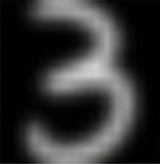
\includegraphics[width=16px]{chapter1/usps3.png}
        
\includegraphics[width=16px]{chapter1/usps6.png}
        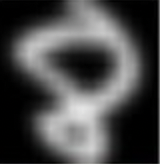
\includegraphics[width=16px]{chapter1/usps8.png}                              & 
\includegraphics[width=16px]{chapter1/svhn3.png}
        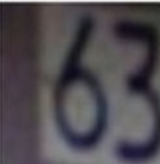
\includegraphics[width=16px]{chapter1/svhn6.png}
        
\includegraphics[width=16px]{chapter1/svhn8.png}                                                                                                                                                          \\
        \midrule
        MNIST                                                                         & \multirow{2}{*}{\textbf{99.17\%}}                 & \multirow{2}{*}{78.08\%}          & \multirow{2}{*}{31.50\%}          \\
        
\includegraphics[width=16px]{chapter1/mnist3.png}
        
\includegraphics[width=16px]{chapter1/mnist6.png}
        
\includegraphics[width=16px]{chapter1/mnist8.png}                             &                                                   &                                   &                                   \\
        USPS                                                                          & \multirow{2}{*}{57.10\%}                          & \multirow{2}{*}{\textbf{95.42\%}} & \multirow{2}{*}{26.94\%}          \\
        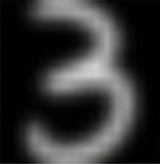
\includegraphics[width=16px]{chapter1/usps3.png}
        
\includegraphics[width=16px]{chapter1/usps6.png}
        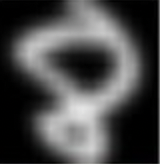
\includegraphics[width=16px]{chapter1/usps8.png}                              &                                                   &                                   &                                   \\
        SVHN                                                                          & \multirow{2}{*}{61.92\%}                          & \multirow{2}{*}{64.28\%}          & \multirow{2}{*}{\textbf{89.52\%}} \\
        
\includegraphics[width=16px]{chapter1/svhn3.png}
        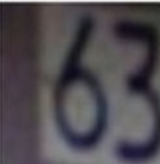
\includegraphics[width=16px]{chapter1/svhn6.png}
        
\includegraphics[width=16px]{chapter1/svhn8.png}                              &                                                   &                                   &                                   \\
        \bottomrule
    \end{tabular}
    \caption{Precisión que se obtiene al aplicar un modelo LeNet5 entrenado con otros conjuntos de datos de dígitos.}
    \label{tab:lenet-distintos-datasets}
\end{table}

En conclusión, debido a que la escritura de los números en los telegramas puede variar de elección en elección y a que
los datos de entrenamiento no son suficientes para una clasificación precisa en este contexto, se necesita recurrir a
técnicas más complejas de entrenamiento que permitan al modelo adaptarse a diferentes dominios. La adaptación de
dominio es una técnica que busca reducir el efecto del sesgo de los datos y hacer que el modelo sea más robusto ante
las variaciones en la escritura de los números. En la actualidad, no existen trabajos publicados que comparen
diferentes técnicas de adaptación de dominio para la digitalización de telegramas en Argentina, lo que sugiere una
oportunidad para investigar y desarrollar modelos más efectivos para este propósito.

\section{Objetivos}

El objetivo general de esta tesis es poder clasificar los dígitos de los votos en las elecciones legislativas de la
provincia de Santa Fe del año 2021 mediante adaptación de dominio de forma que el modelo generalice y no dependa de un
etiquetado de los datos. El enfoque se centrará en explorar y comparar diferentes técnicas de adaptación de dominio con
el fin de lograr un modelo robusto que pueda generalizar en diferentes contextos y escenarios electorales. Con esto se
contribuye a mejorar la transparencia y eficiencia en los procesos electorales en Argentina y sentar las bases para el
desarrollo de soluciones similares para el resto de las provincias y la nación.

Los objetivos específicos para lograr el objetivo planteado son los siguientes:

\begin{itemize}
    \item Armar el proceso de extracción, transformación y carga (ETL) de los telegramas, con el propósito de segmentar y limpiar
          de manera efectiva los dígitos. Los datos utilizados serán obtenidos de fuentes oficiales del estado
          argentino\footnote{\href{https://op.elecciones.gob.ar/telegramas/generales2021/}{https://op.elecciones.gob.ar/telegramas/generales2021/}.}.
          En el anexo \ref{anexo:telegrama} se adjunta un ejemplo de uno de ellos.
    \item Entrenar distintas arquitecturas de redes convolucionales mediante técnicas de adaptación de dominio.
    \item Analizar y evaluar las métricas relevantes para seleccionar el mejor modelo.
    \item Detectar oportunidades de mejora en el proceso eleccionario respecto a los telegramas.
\end{itemize}

\section{Estructura de la tesis}

Esta tesis se encuentra organizado con la siguiente estructura:

\begin{itemize}
    \item Capítulo 2: Marco teórico del reconocimiento de dígitos, redes neuronales, aprendizaje por transferencia y adaptación
          de dominio.
    \item Capítulo 3: Metodología del trabajo realizado sobre los telegramas de las elecciones de Santa Fe. Proceso de
          extracción, transformación y limpieza de los mismos. Diseño experimental y métricas de evaluación.
    \item Capítulo 4: Análisis de resultados. Análisis de métricas, espacios latentes obtenidos y errores observados.
    \item Capítulo 5: Conclusiones del trabajo, mejoras planteadas y futuras investigaciones.
\end{itemize}
\chapter{Marco te\'orico}
\label{Chapter2}

En este capítulo se presenta una visión general de la bibliografía relacionada al objetivo del presente trabajo. En la
primera sección se detalla una revisión de trabajos relacionados. En ... % TODO: completar

\section{Reconocimiento de d\'igitos}

% otro
El reconocimiento de dígitos escritos a mano por parte de las computadoras es una tarea que ha fascinado a la comunidad
de aprendizaje automático durante muchos años. Aunque el reconocimiento de dígitos escritos a mano es una tarea
relativamente sencilla para los humanos, ha sido un desafío para las computadoras debido a la gran variabilidad en la
forma en que los dígitos son escritos por diferentes personas.

Los primeros estudios psicológicos sobre el reconocimiento de dígitos escritos a mano se llevaron a cabo a principios
del siglo XX (Gross, 1914). Estos estudios investigaron cómo los humanos reconocen dígitos escritos a mano y
proporcionaron información valiosa sobre las características visuales que son importantes para el reconocimiento de
dígitos.

A medida que la tecnología de las computadoras ha avanzado, se han desarrollado diversos enfoques para el
reconocimiento de dígitos escritos a mano por parte de las computadoras. Uno de los primeros enfoques fue presentado
por H. B. Friedman en 1963 (Friedman, 1963). En este trabajo, se utilizó una red neuronal simple para reconocer dígitos
escritos a mano en tarjetas perforadas. Aunque el rendimiento de la red fue bastante bajo, este trabajo marcó el inicio
de la investigación en el reconocimiento de dígitos escritos a mano por parte de las computadoras.

A mediados de la década de 1980, se presentó un enfoque importante para el reconocimiento de dígitos escritos a mano
llamado "Sistema Neuronal de Reconocimiento de Dígitos" o "NDN" (LeCun et al., 1989). Este sistema utilizó una red
neuronal de varias capas y fue entrenado utilizando el método de retropropagación del error. El NDN tuvo un rendimiento
significativamente mejor que los enfoques anteriores y sentó las bases para el desarrollo de sistemas de reconocimiento
de dígitos escritos a mano más sofisticados.

En la década de 1990, se presentaron varios enfoques basados en el aprendizaje automático para el reconocimiento de
dígitos escritos a mano que tuvieron un rendimiento aún mejor. Un ejemplo es el "Sistema de Procesamiento de Imágenes
de Dígitos Escritos a Mano" o "HWDS" (Lecun et al., 1998). Este sistema utilizó una red neuronal de varias capas y se
entrenó utilizando el método de retropropagación del error con un conjunto de datos de imágenes de dígitos escritos a
mano muy grande. El HWDS tuvo un rendimiento excepcional y se convirtió en un estándar de la industria en el
reconocimiento de dígitos escritos a mano.

En la última década, el aprendizaje profundo ha revolucionado el reconocimiento de dígitos escritos a mano y ha llevado
a un rendimiento aún mejor. Un ejemplo de esto es el "Modelo de Deep Learning para el Reconocimiento de Dígitos
Escritos a Mano" o "Mnist-DNN" (Ciresan et al., 2012). Este modelo utilizó una red neuronal profunda y fue entrenado
utilizando un conjunto de datos de imágenes de dígitos escritos a mano muy grande. El Mnist-DNN tuvo un rendimiento
excepcional y es ampliamente utilizado en la industria y la investigación.

En resumen, el reconocimiento de dígitos escritos a mano por parte de las computadoras ha evolucionado
significativamente a lo largo de los años. Desde los primeros estudios psicológicos hasta el aprendizaje profundo
actual, se ha avanzado mucho en el entendimiento de cómo las computadoras pueden reconocer dígitos escritos a mano y se
han desarrollado diversos enfoques para abordar esta tarea.

\section{Redes Neuronales}
\cite{mcculloch1943logical} estudiaron y propusieron un modelo del comportamiento de la
neurona biológica. La neurona artificial que propusieron fue un sistema binario que consiste en que si la suma de entradas excitatorias supera un umbral de activación, y además no
hay una entrada inhibitoria, la neurona se activa y emite una respuesta; en caso contrario, la neurona no se activa.

En \citeyear{hebb1949organization} se propone que estas redes podían aprender. Este hecho estaba relacionado con la
conductividad de la sinapsis. Así, la repetida activación de una neurona por otra, a través de una sinapsis
determinada, aumenta su conductividad y la hace más propensa a ser activada sucesivamente, induciendo a la formación de
un circuito de neuronas estrechamente conectadas entre sí \parencite{hebb1949organization}.

Años más tarde, \cite{rosenblatt1958perceptron} propone un modelo de neurona llamadas perceptrones basadas en el modelo
de McCulloch-Pitts. El mayor logro de Rosenblatt fue que pudo demostrar que, flexibilizando algunas de las reglas de la
McCulloch-Pitts (la inhibición absoluta, la contribución igual de todas las entradas, etc), las neuronas artificiales
podían aprender de los datos. Y lo que es más importante, ideó un algoritmo de aprendizaje supervisado para este modelo
de neurona que permitía averiguar los pesos correctos directamente a partir de los datos de entrenamiento. La sencillez
y eficacia de este algoritmo de aprendizaje para problemas linealmente separables son algunas de las razones clave por
las que se hizo tan popular a finales de los años cincuenta y principios de los sesenta. Sin embargo, esta popularidad
hizo que Rosenblatt exagerara la capacidad de aprendizaje de su perceptrón, dando lugar a expectativas poco realistas
en la comunidad científica y/o también difundidas por los medios de comunicación.

En \citeyear{minsky1969perceptrons}, se publica un libro en el cual se expone la naturaleza lineal de los perceptrones
y de sus limitadas capacidades \parencite{minsky1969perceptrons}. A raíz de este evento es que se inicia el denominado "invierno de la inteligencia
artificial" de los 1980s, donde cesó el interés de la comunidad por los modelos conexionistas.

La contribución más importante en la reemergencia del conexionismo en los años ochenta fue la técnica {\it
backpropagation} desarrollada por \cite{rumelhart1986learning}. En realidad, esta técnica fue desarrollada inicialmente
por \cite{werbos1974beyond} y después redescubierta por varios grupos de investigadores \parencite{lecun1985learning, rumelhart1986learning}. Este algoritmo abrió las puertas al uso práctico de las redes
neuronales en un sinfín de campos. Las más "simples" en la práctica son las llamadas redes multicapa alimentadas hacia
delante ({\it feed forward}) entrenadas con {\it backpropagation}, también referidas como perceptrones mutlicapa {\it
        MLP}.

En \citeyear{funahashi1989approximate}, se demuestra teóricamente que una red de este tipo, con una capa oculta, el
suficiente número de nodos y entrenada con {\it backpropagation}, puede aproximar cualquier función continua con
cualquier grado de precisión \parencite{funahashi1989approximate}.

\subsection{Redes densas}
Como se detalló anteriormente, los perceptrones son modelos lineales incapaces de resolver problemas que no sean
linealmente separables por un hiperplano. Una forma de solventar esta situación es encadenar un conjunto de
perceptrones para crear redes neuronales densas (ver figura \ref{fig:nn}). La predicción $\hat{y}$ de una red es una
generalización directa de la predicción de un perceptrón. Primero se calculan las activaciones $a_i^1$ de los nodos de
la capa oculta $h_i^1$ en función de las entradas $x_i$ y los pesos de entrada $w_i^1$. Luego, se calculan las
activaciones $a_i^2$ de la unidad de salida $h_1^2$ dadas las activaciones de la capa anterior y los pesos $w_i^2$.

\begin{figure}[H]
    \centering

    \tikzset{every picture/.style={line width=0.75pt}} %set default line width to 0.75pt        

    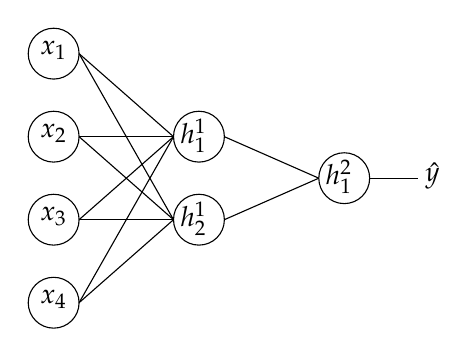
\begin{tikzpicture}[x=0.75pt,y=0.75pt,yscale=-1,xscale=1]
        %uncomment if require: \path (0,300); %set diagram left start at 0, and has height of 300

        %Shape: Circle [id:dp4714623984365989] 
        \draw   (0,12.25) .. controls (0,5.48) and (5.48,0) .. (12.25,0) .. controls (19.02,0) and (24.5,5.48) .. (24.5,12.25) .. controls (24.5,19.02) and (19.02,24.5) .. (12.25,24.5) .. controls (5.48,24.5) and (0,19.02) .. (0,12.25) -- cycle ;

        %Shape: Circle [id:dp25434586654127544] 
        \draw   (0,52.25) .. controls (0,45.48) and (5.48,40) .. (12.25,40) .. controls (19.02,40) and (24.5,45.48) .. (24.5,52.25) .. controls (24.5,59.02) and (19.02,64.5) .. (12.25,64.5) .. controls (5.48,64.5) and (0,59.02) .. (0,52.25) -- cycle ;

        %Shape: Circle [id:dp9726011815419306] 
        \draw   (0,92.25) .. controls (0,85.48) and (5.48,80) .. (12.25,80) .. controls (19.02,80) and (24.5,85.48) .. (24.5,92.25) .. controls (24.5,99.02) and (19.02,104.5) .. (12.25,104.5) .. controls (5.48,104.5) and (0,99.02) .. (0,92.25) -- cycle ;

        %Shape: Circle [id:dp2291699685520565] 
        \draw   (0,132.25) .. controls (0,125.48) and (5.48,120) .. (12.25,120) .. controls (19.02,120) and (24.5,125.48) .. (24.5,132.25) .. controls (24.5,139.02) and (19.02,144.5) .. (12.25,144.5) .. controls (5.48,144.5) and (0,139.02) .. (0,132.25) -- cycle ;

        %Shape: Circle [id:dp14614955000159813] 
        \draw   (70,52.25) .. controls (70,45.48) and (75.48,40) .. (82.25,40) .. controls (89.02,40) and (94.5,45.48) .. (94.5,52.25) .. controls (94.5,59.02) and (89.02,64.5) .. (82.25,64.5) .. controls (75.48,64.5) and (70,59.02) .. (70,52.25) -- cycle ;

        %Shape: Circle [id:dp8388103519245029] 
        \draw   (70,92.25) .. controls (70,85.48) and (75.48,80) .. (82.25,80) .. controls (89.02,80) and (94.5,85.48) .. (94.5,92.25) .. controls (94.5,99.02) and (89.02,104.5) .. (82.25,104.5) .. controls (75.48,104.5) and (70,99.02) .. (70,92.25) -- cycle ;

        %Shape: Circle [id:dp7556907650297429] 
        \draw   (140,72.25) .. controls (140,65.48) and (145.48,60) .. (152.25,60) .. controls (159.02,60) and (164.5,65.48) .. (164.5,72.25) .. controls (164.5,79.02) and (159.02,84.5) .. (152.25,84.5) .. controls (145.48,84.5) and (140,79.02) .. (140,72.25) -- cycle ;

        %Straight Lines [id:da8929189573178169] 
        \draw    (24.5,12.25) -- (70,52.25) ;
        %Straight Lines [id:da5905797689118961] 
        \draw    (24.5,52.25) -- (70,52.25) ;
        %Straight Lines [id:da8059054934899097] 
        \draw    (24.5,92.25) -- (70,52.25) ;
        %Straight Lines [id:da18480058250239084] 
        \draw    (24.5,132.25) -- (70,52.25) ;
        %Straight Lines [id:da9649216528295181] 
        \draw    (24.5,12.25) -- (70,92.25) ;
        %Straight Lines [id:da2593081377394073] 
        \draw    (24.5,52.25) -- (70,92.25) ;
        %Straight Lines [id:da23945860731626256] 
        \draw    (24.5,92.25) -- (70,92.25) ;
        %Straight Lines [id:da45284543126132815] 
        \draw    (24.5,132.25) -- (70,92.25) ;
        %Straight Lines [id:da8439890580329283] 
        \draw    (94.5,52.25) -- (140,72.25) ;
        %Straight Lines [id:da026411209066727226] 
        \draw    (94.5,92.25) -- (140,72.25) ;
        %Straight Lines [id:da46511217961352624] 
        \draw    (164.5,72.25) -- (187.75,72.25) ;

        % Text Node
        \draw (4.5,5) node [anchor=north west][inner sep=0.75pt]    {$x_{1}$};
        % Text Node
        \draw (4.5,45) node [anchor=north west][inner sep=0.75pt]    {$x_{2}$};
        % Text Node
        \draw (4.5,85) node [anchor=north west][inner sep=0.75pt]    {$x_{3}$};
        % Text Node
        \draw (4.5,125) node [anchor=north west][inner sep=0.75pt]    {$x_{4}$};
        % Text Node
        \draw (72,42.4) node [anchor=north west][inner sep=0.75pt]    {$h_{1}^{1}$};
        % Text Node
        \draw (72,82.4) node [anchor=north west][inner sep=0.75pt]    {$h_{2}^{1}$};
        % Text Node
        \draw (142,62.4) node [anchor=north west][inner sep=0.75pt]    {$h_{1}^{2}$};
        % Text Node
        \draw (190,63.4) node [anchor=north west][inner sep=0.75pt]    {$\hat{y}$};

    \end{tikzpicture}
    \caption{Red neuronal con una capa de entrada de 4 características, una capa oculta de 2 neuronas y una capa de salida con 1 neurona.}
    \label{fig:nn}
\end{figure}

La única diferencia entre este cálculo y el del perceptrón es que las unidades ocultas calculan una función no lineal
de sus entradas. Generalmente es llamada como {\it función de activación} o {\it función de enlace}. Formalmente, si
$w_{i,d}$ son los pesos que conectan las entradas $d$ a la unidad oculta $i$, entonces la activación de la unidad $i$
se calcula como:

\begin{align}
    h_i = f(\mathbf{w}_i \cdot \mathbf{x} + b_i)
\end{align}

Donde $f$ es la función de activación, $\mathbf{w}_i$ es el vector de pesos que alimentan el nodo $i$ y $b_i$ es el
término de {\it bias}. Existen múltiples funciones de activación, las más comunes son:

\begin{itemize}
    \item Tangente hiperbólica: $f(x) = tanh(x)$
    \item Función sigmoidea: $f(x) = \frac{1}{1+exp(-x)}$
    \item ReLU: $f(x) = max(0, x)$
\end{itemize}

\subsection{Convolucionales}
Las redes neuronales convolucionales (CNNs, por sus siglas en inglés) son un tipo de modelo de aprendizaje automático
que ha demostrado ser muy efectivo en tareas de procesamiento de imágenes y lenguaje natural. Estas redes son una
variante de las redes neuronales feedforward, que constan de varias capas de neuronas interconectadas. Lo que
diferencia a las CNNs de otras redes neuronales es su uso de capas de convolución, que permiten a la red aprender
características espaciales de los datos de entrada de manera automática.

Una de las principales ventajas de las CNNs es que son capaces de procesar datos con una gran cantidad de dimensiones,
como imágenes con altura, anchura y profundidad (canales de color). Esto se debe a que las capas de convolución son
capaces de realizar operaciones de filtrado sobre los datos de entrada, permitiendo a la red aprender características
específicas de los datos de manera eficiente. Además, las CNNs tienen la capacidad de generalizar de manera efectiva,
lo que significa que son capaces de realizar buenas predicciones en conjuntos de datos desconocidos.

Un ejemplo de aplicación de las CNNs es en el reconocimiento de objetos en imágenes. Al entrenar una red con un gran
número de imágenes etiquetadas, la red puede aprender a reconocer patrones y características específicas de cada clase
de objeto. Luego, al presentarle una imagen desconocida, la red puede utilizar lo que ha aprendido para clasificar la
imagen en una de las clases de objetos que ha visto durante el entrenamiento.

Las CNNs han demostrado ser muy efectivas en una gran variedad de tareas, como la clasificación de imágenes, el
procesamiento de lenguaje natural y el análisis de sentimientos. Algunos ejemplos de papers que abordan el uso de CNNs
son "Very Deep Convolutional Networks for Large-Scale Image Recognition" (Simonyan y Zisserman, 2014), "Convolutional
Neural Networks for Sentence Classification" (Kim, 2014) y "Convolutional Neural Networks for Sentiment Analysis of
Short Texts" (Zhang y Lee, 2015).

% Otro
Una de las principales limitaciones de las redes feedforward densas es que no son muy buenas para trabajar con datos
que tienen una estructura espacial, como imágenes o audio. Esto se debe a que las redes feedforward densas tratan a
todas las entradas de manera aislada, sin tener en cuenta las relaciones entre ellas. Esto puede llevar a que la red no
sea capaz de detectar patrones o características importantes en los datos, lo que puede limitar su rendimiento.

Para solucionar este problema, surgió la idea de utilizar redes neuronales convolucionales (CNN). Estas redes se basan
en la idea de utilizar capas de neuronas que comparten pesos y realizan una operación de convolución en los datos de
entrada. Esto permite que la red tenga una mayor capacidad para detectar patrones y características en los datos, ya
que las neuronas de las capas de convolución están compartiendo información y pueden detectar patrones a diferentes
escalas y en diferentes posiciones de los datos.

Además, las CNN también tienen capas de pooling, que se encargan de seleccionar las características más importantes de
los datos y reducir su tamaño, lo que permite que la red tenga un mejor rendimiento y sea más eficiente.

En resumen, las redes neuronales convolucionales surgieron como una mejora de las redes feedforward densas debido a su
capacidad para trabajar con datos que tienen una estructura espacial, como imágenes o audio, y detectar patrones y
características importantes en ellos de manera más eficiente.

% Otro
Las convoluciones en una red neuronal son una técnica utilizada para detectar patrones y características en los datos
de entrada. Esto se hace mediante el uso de una máscara o filtro que se desliza por los datos y realiza una operación
de convolución para combinar los valores de los datos con los pesos del filtro.

Matemáticamente, la operación de convolución se puede representar como:

$$ (f * g)(x) = \int_{-\infty}^{\infty} f(t)g(x-t) dt $$

Donde $f$ y $g$ son dos funciones y $*$ es el operador de convolución. Esta operación consiste en desplazar la función
$g$ a través de la función $f$ y multiplicar cada valor de $f$ por el valor de $g$ en esa posición. El resultado de la
operación de convolución es una nueva función que refleja la combinación de los valores de $f$ y $g$.

En el contexto de una red neuronal, el filtro o máscara se utiliza para detectar patrones o características en los
datos de entrada. Cada neurona de la capa de convolución está conectada a un subconjunto de los datos de entrada y
realiza una operación de convolución con ellos utilizando el filtro asociado. Los pesos del filtro se actualizan
durante el proceso de aprendizaje para mejorar la capacidad de la red para detectar patrones y características
importantes en los datos.

Referencias:

Lecun, Y., Bottou, L., Bengio, Y., \& Haffner, P. (1998). Gradient-based learning applied to document recognition.
Proceedings of the IEEE, 86(11), 2278-2324. Goodfellow, I., Bengio, Y., \& Courville, A. (2016). Deep learning. MIT
Press.

% Otro
Para entrenar las capas convolucionales de una red neuronal artificial, se utiliza un proceso conocido como
backpropagation. Este proceso consiste en calcular el error entre la salida de la red y la salida esperada para un
conjunto de datos de entrenamiento y utilizar este error para actualizar los pesos de la red de manera que el error
disminuya.

Matemáticamente, el proceso de backpropagation se puede representar como:

$$ \frac{\partial E}{\partial w_{ij}} = \frac{\partial E}{\partial y_i} \frac{\partial y_i}{\partial w_{ij}} $$

Donde $E$ es el error, $y_i$ es la salida de la neurona $i$, $w_{ij}$ es el peso de la conexión entre la neurona $i$ y
la neurona $j$, y $\frac{\partial}{\partial}$ es el operador de derivada parcial.

El proceso de backpropagation se repite varias veces para cada conjunto de datos de entrenamiento y se utiliza para
actualizar los pesos de la red de manera que el error disminuya y la red pueda realizar tareas de manera más precisa.

\subsection{Arquitecturas}

Hay distintos tipos de arquitecturas de redes neuronales convolucionales debido a que cada una tiene diferentes
fortalezas y debilidades en términos de capacidad de generalización, extracción de características y rendimiento.
Algunos factores que pueden influir en la elección de una arquitectura en particular incluyen:

Tamaño de los datos de entrada: para procesar grandes conjuntos de datos, es posible que se necesite una red con una
mayor capacidad de procesamiento y una mayor cantidad de parámetros.

Nivel de detalle de las características: algunas arquitecturas pueden ser más eficientes para detectar características
a diferentes escalas y en diferentes posiciones, mientras que otras pueden tener una mayor capacidad para detectar
patrones complejos.

Nivel de generalización: algunas arquitecturas pueden ser más capaces de generalizar a datos nuevos y menos vistos
durante el entrenamiento, mientras que otras pueden ser más propensas a sobreajuste.

Requerimientos de tiempo y recursos: algunas arquitecturas pueden requerir más tiempo y recursos para entrenar y
evaluar, lo que puede ser un factor importante a considerar dependiendo de los objetivos del proyecto.

% otro

Existen distintos tipos de arquitecturas de redes neuronales convolucionales debido a que cada una tiene diferentes
fortalezas y debilidades en términos de capacidad de generalización, extracción de características y rendimiento (LeCun
et al., 2015). Algunos factores que pueden influir en la elección de una arquitectura en particular incluyen el tamaño
de los datos de entrada, el nivel de detalle de las características que se desean extraer, el nivel de generalización
que se requiere y los requerimientos de tiempo y recursos (He et al., 2016).

Una arquitectura de red neuronal convolucional simple es la red LeNet, que fue propuesta por LeCun et al. (1998) y es
utilizada comúnmente para clasificación de imágenes. Esta red consta de dos capas de convolución seguidas por dos capas
densas y una capa de salida, y fue utilizada con éxito para el reconocimiento de números escritos a mano en el conjunto
de datos MNIST.

Por otro lado, una arquitectura de red neuronal convolucional más compleja es la red ResNet, propuesta por He et al.
(2016). Esta red utiliza una técnica llamada "saltos de conexión directa" para evitar el problema de la degradación del
rendimiento en redes profundas y ha demostrado tener una excelente capacidad de generalización en tareas de
clasificación de imágenes.

En general, al elegir una arquitectura de red neuronal convolucional es importante tener en cuenta los factores
mencionados anteriormente y evaluar cuál es la que mejor se ajusta a las necesidades del problema a resolver y a los
datos de entrada disponibles.

Referencias:

He, K., Zhang, X., Ren, S., \& Sun, J. (2016). Deep residual learning for image recognition. In Proceedings of the IEEE
conference on computer vision and pattern recognition (pp. 770-778).

LeCun, Y., Bottou, L., Bengio, Y., \& Haffner, P. (1998). Gradient-based learning applied to document recognition.
Proceedings of the IEEE, 86(11), 2278-2324.

LeCun, Y., Bengio, Y., \& Hinton, G. (2015). Deep learning. Nature, 521(7553), 436-444.

\subsubsection{LeNet}
% Otro
La red LeNet fue propuesta por Yann LeCun, Léon Bottou, Yoshua Bengio y Patrick Haffner en 1998 y es una de las
primeras redes neuronales convolucionales en ser utilizada con éxito para el reconocimiento de imágenes (LeCun et al.,
1998). Esta red consta de dos capas de convolución seguidas por dos capas densas y una capa de salida, y fue utilizada
con éxito para el reconocimiento de números escritos a mano en el conjunto de datos MNIST.

La red LeNet tuvo varias versiones a lo largo de los años, y cada una de ellas presentó mejoras en términos de
rendimiento y capacidad de generalización. Por ejemplo, en 2002 se presentó la red LeNet-4, que incluyó una capa
adicional de convolución y una capa de pooling (S. Savage, 2002).

En general, la red LeNet tuvo un gran impacto en el campo de la inteligencia artificial y ha sido utilizada como base
para el desarrollo de muchas otras redes neuronales convolucionales. Ha demostrado ser una herramienta muy efectiva
para el reconocimiento de imágenes y ha sido utilizada en aplicaciones como el reconocimiento de escritura a mano, el
reconocimiento de caracteres y el análisis de imágenes médicas.

Referencias:

LeCun, Y., Bottou, L., Bengio, Y., \& Haffner, P. (1998). Gradient-based learning applied to document recognition.
Proceedings of the IEEE, 86(11), 2278-2324.

Savage, S. (2002). LeNet-4: an unsupervised neural network. arXiv preprint cs/0206061.

\subsubsection{ResNet}
% Otro
La red ResNet (short for Residual Network) fue propuesta por Kaiming He, Xiangyu Zhang, Shaoqing Ren y Jian Sun en 2015
y es una de las arquitecturas de redes neuronales más populares y exitosas en el campo de la visión por computadora (He
et al., 2015). Esta red utiliza una técnica llamada "saltos de conexión directa" para evitar el problema de la
degradación del rendimiento en redes profundas, que es un fenómeno que ocurre cuando el rendimiento de una red
disminuye a medida que aumenta su profundidad.

La red ResNet se ha utilizado con éxito en varias tareas de visión por computadora, como la clasificación de imágenes,
la detección de objetos y el seguimiento de movimientos. Ha demostrado tener una excelente capacidad de generalización
y ha obtenido resultados sobresalientes en varias competencias de visión por computadora, como la competencia ImageNet
de 2015.

La red ResNet ha tenido varias versiones a lo largo de los años, y cada una de ellas presentó mejoras en términos de
rendimiento y capacidad de generalización.

% Otro
La red ResNet (short for Residual Network) surge como una forma de abordar el problema de la degradación del
rendimiento en redes profundas, que es un fenómeno que ocurre cuando el rendimiento de una red disminuye a medida que
aumenta su profundidad (He et al., 2015). Esto es un problema importante en el campo de la visión por computadora, ya
que muchas tareas requieren redes profundas para obtener buenos resultados, pero a menudo se encuentra que el
rendimiento empeora a medida que se aumenta la profundidad.

La red ResNet utiliza una técnica llamada "saltos de conexión directa" para evitar el problema de la degradación del
rendimiento. Esta técnica consiste en agregar una conexión directa entre la entrada y la salida de cada bloque de la
red, en lugar de utilizar solo capas completamente conectadas. Esto permite que la red pueda aprender una función de
identidad y luego aprender cualquier cambio necesario a partir de eso, lo que hace que sea más fácil para la red
aprender funciones complejas.

La red ResNet ha tenido varias versiones a lo largo de los años, y cada una de ellas presentó mejoras en términos de
rendimiento y capacidad de generalización. Algunas de las versiones más populares son ResNet-18, ResNet-34 y ResNet-50,
que tienen 18, 34 y 50 capas respectivamente. Estas versiones se han utilizado con éxito en varias tareas de visión por
computadora y han obtenido resultados sobresalientes en varias competencias de visión por computadora.

Referencias:

He, K., Zhang, X., Ren, S., \& Sun, J. (2015). Deep residual learning for image recognition. In Proceedings of the IEEE
conference on computer vision and pattern recognition (pp. 770-778).

\section{Aprendizaje por transferencia}
% Otro
El aprendizaje por transferencia es una técnica de aprendizaje automático que consiste en utilizar lo que se ha
aprendido en una tarea para mejorar el rendimiento en otra tarea relacionada (Pan, Yang, \& McOwan, 2010). Esta técnica
se aplica comúnmente en el contexto de redes neuronales y se basa en la idea de que algunos conocimientos adquiridos en
una tarea pueden ser reutilizados en otra tarea, lo que permite que la red aprenda de manera más eficiente y con menos
datos.

En el caso de las redes neuronales, el aprendizaje por transferencia puede utilizarse de varias maneras, como por
ejemplo:

Entrenar una red en una tarea y luego utilizarla como inicialización para otra tarea: en este caso, la red se entrena
inicialmente en una tarea y luego se utiliza como punto de partida para entrenar otra red en una tarea diferente. Esto
permite que la red aprenda de manera más rápida y con menos datos, ya que ya ha adquirido algunos conocimientos en la
primera tarea.

Utilizar capas de una red entrenada en una tarea como capas fijas en otra tarea: en este caso, se utilizan las capas de
una red entrenada en una tarea como capas fijas en otra red que se entrena en una tarea diferente. Esto permite que la
red aprenda de manera más rápida y con menos datos, ya que ya ha adquirido algunos conocimientos en la primera tarea.

% Otro

El aprendizaje por transferencia es una técnica de aprendizaje automático que consiste en utilizar lo que se ha
aprendido en una tarea para mejorar el rendimiento en otra tarea relacionada (Pan, Yang, \& McOwan, 2010). En el
contexto de las redes neuronales, el aprendizaje por transferencia se puede llevar a cabo de varias maneras, como el
pre-training y el fine-tuning.

El pre-training es una técnica de aprendizaje por transferencia en la que se entrena una red en una tarea y luego se
utiliza como punto de partida para entrenar otra red en una tarea diferente (Erhan, Bengio, Courville, \& Vincent,
2010). Esto permite que la red aprenda de manera más rápida y con menos datos, ya que ya ha adquirido algunos
conocimientos en la primera tarea. El pre-training se puede llevar a cabo de varias maneras, como por ejemplo
entrenando una red en un conjunto de datos de gran tamaño y luego utilizándola como inicialización para una tarea
específica.

El fine-tuning es una técnica de aprendizaje por transferencia en la que se utilizan las capas de una red entrenada en
una tarea como capas fijas en otra red que se entrena en una tarea diferente (Yosinski, Clune, Bengio, \& Lipson,
2014). Esto permite que la red aprenda de manera más rápida y con menos datos.

% Otro
El pre-training es una técnica de aprendizaje por transferencia en la que se entrena una red en una tarea y luego se
utiliza como punto de partida para entrenar otra red en una tarea diferente (Erhan, Bengio, Courville, \& Vincent,
2010). Esto permite que la red aprenda de manera más rápida y con menos datos, ya que ya ha adquirido algunos
conocimientos en la primera tarea.

El pre-training se puede llevar a cabo de varias maneras, como por ejemplo entrenando una red en un conjunto de datos
de gran tamaño y luego utilizándola como inicialización para una tarea específica. Esto se ha utilizado con éxito en
varias tareas de aprendizaje automático, como la clasificación de imágenes y el procesamiento del lenguaje natural
(Shin et al., 2016; Howard et al., 2018).

El pre-training también se ha utilizado con éxito en el contexto de redes neuronales profundas, donde ha demostrado ser
una técnica efectiva para mejorar el rendimiento y la capacidad de generalización de las redes (Girshick et al., 2014).
En particular, el pre-training ha demostrado ser útil para reducir el número de datos necesarios para entrenar una red
y para mejorar el rendimiento en tareas con conjuntos de datos pequeños o de baja calidad.

Referencias:

Erhan, D., Bengio, Y., Courville, A., \& Vincent, P. (2010). Why does unsupervised pre-training help deep learning? In
Proceedings of the 13th international conference on artificial intelligence and statistics (pp. 217-224).

Girshick, R., Donahue, J., Darrell, T., \& Malik, J. (2014). Rich feature hierarchies for accurate object detection and
semantic segmentation. In Proceedings of the IEEE conference on computer vision and pattern recognition (pp. 580-587).

Howard, J., Sandler, M., Chu, G., Chen, L., Chen, B., Tan, M., \& Wang, W. (2018). MobileNets: Efficient convolutional
neural networks for mobile vision applications. arXiv preprint arXiv:1704.04861.

Shin, H., Valveny

% otro
uego fine-tunearlo para clasificar imágenes de plantas utilizando un conjunto de datos de imágenes de plantas más
pequeño. En este caso, el modelo ya tiene una comprensión básica de cómo procesar imágenes y podemos ajustar sus
parámetros para que se adapte mejor a nuestra tarea específica de clasificación de plantas.

El "pre-training" es una forma de aprendizaje por transferencia donde se entrena un modelo en una tarea generalizada y
luego se utiliza como base para resolver tareas más específicas. Por ejemplo, podríamos entrenar un modelo en una tarea
genérica de procesamiento del lenguaje natural y luego utilizar ese modelo como base para resolver tareas más
específicas como la clasificación de sentimentos o la traducción de idiomas.

En resumen, el "fine-tuning" implica ajustar los parámetros de un modelo previamente entrenado para adaptarlo a una
tarea específica, mientras que el "pre-training" implica entrenar un modelo en una tarea genérica y luego utilizarlo
como base para resolver tareas más específicas.

% Otro

El aprendizaje por transferencia o "transfer learning" se refiere a la práctica de utilizar un modelo previamente
entrenado en una tarea específica y reutilizar parte o todo ese conocimiento para resolver una tarea diferente (Pan \&
Yang, 2010). Esta técnica ha ganado popularidad en los últimos años debido a la creciente cantidad de datos disponibles
y a la necesidad de entrenar modelos más complejos y de mayor rendimiento (Torrey \& Shavlik, 2010).

Hay varias formas de hacer esto, como el "fine-tuning" y el "pre-training". El "fine-tuning" implica la adaptación de
un modelo previamente entrenado para resolver una tarea específica, ajustando sus parámetros en lugar de entrenar un
nuevo modelo desde cero (Yosinski et al., 2014). Esto se hace generalmente en el caso de tener un conjunto de datos
pequeño y utilizar un modelo previamente entrenado en un conjunto de datos más grande (Donahue et al., 2014). Por
ejemplo, podríamos utilizar un modelo previamente entrenado en un conjunto de datos de imágenes de animales y luego
fine-tunearlo para clasificar imágenes de plantas utilizando un conjunto de datos de imágenes de plantas (Girshick et
al., 2014).

El "pre-training" es otra forma de aprendizaje por transferencia que implica entrenar un modelo en un conjunto de datos
muy grande y luego reutilizar parte o todo ese conocimiento para resolver una tarea específica (Collobert \& Weston,
2008). El objetivo es aprovechar el conocimiento aprendido por el modelo sobre el conjunto de datos general para
mejorar el rendimiento en la tarea específica (Erhan et al., 2010). Por ejemplo, podríamos entrenar un modelo en un
conjunto de datos de texto muy grande y luego utilizar ese modelo pre-entrenado para resolver tareas de procesamiento
del lenguaje natural, como la clasificación de opiniones o la traducción (Mikolov et al., 2013).

En resumen, el fine-tuning implica la adaptación de un modelo previamente entrenado a una tarea específica mediante el
ajuste de sus parámetros, mientras que el pre-training involucra el entrenamiento de un modelo en un conjunto de datos
muy grande y luego la reutilización de ese conocimiento para resolver una tarea específica. Ambas técnicas de
aprendizaje por transferencia pueden ser útiles en diferentes escenarios y han demostrado mejorar significativamente el
rendimiento en una variedad de tareas (Shao et al., 2014).
% TODO: hablar de pre-train y fine-tuning

\section{Adaptaci\'on de Dominio}
El {\it pre-entrenamiento} y el {\it fine-tuning} han mejorado considerablemente el estado del arte para diversos
problemas y aplicaciones del machine learning, incluso las redes profundas pre-entrenadas pueden adaptarse fácilmente a
tareas donde se cuenta con una pequeña cantidad de datos etiquetados. Sin embargo, en muchos escenarios prácticos, no
hay datos de entrenamiento etiquetados y, por lo tanto, existe la necesidad de transferir el aprendizaje de una red
profunda desde un dominio de origen en el que se dispone de datos de entrenamiento etiquetados a un dominio de destino
en el que solo existen datos sin etiquetar \parencite{glorot2011domain}. En esta situación, los modelos profundos siguen sufriendo degradaciones de rendimiento debido
al cambio de distribución \parencite{quinonero2008dataset}. Por lo tanto, se propone la {\it adaptación de dominio} para reducir el cambio de
distribución entre los dominios de entrenamiento y de prueba \parencite{jiang2022machine}.

Se han propuesto muchos métodos para la adaptación de dominios, ya sea ponderando o seleccionando muestras del dominio
de origen \parencite{sugiyama2007direct} o buscando una transformación de la distribución de origen a la distribución de destino \parencite{gong2013connecting}. Esta tesis analizar\'a algunos de los m\'etodos m\'as actuales del ultimo caso.

\subsection{Domain Adversarial Neural Network}
Un gran hito al momento de modelar distribuciones es la Red Generativa Adversaria {\it GAN} \parencite{goodfellow2020generative}. Inspirada en estas arquitecturas GAN, la Red Neural Adversaria de Dominio {\it DANN} \parencite{ganin2016domain} consta de dos redes en la adaptación del dominio (figura \ref{fig:dann-esquema}). La primera es
la discriminadora de dominios $\mathcal{D}$ entrenada para distinguir las características de origen de las de destino y
la segunda es una generadora de características $\mathcal{G}$ que se entrena para confundir a $\mathcal{D}$ y
simult\'aneamente ayudar a la red clasificadora $\mathcal{C}$.

\begin{figure}[H]
    \centering

    \tikzset{every picture/.style={line width=0.75pt}} %set default line width to 0.75pt        

    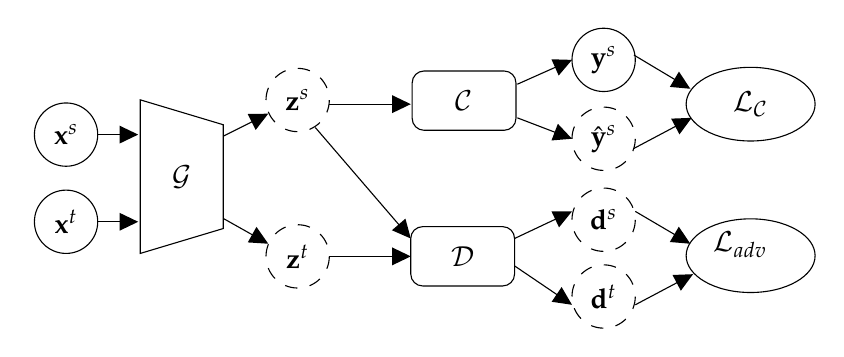
\begin{tikzpicture}[x=0.75pt,y=0.75pt,yscale=-1,xscale=1]
        \draw   (39,64.75) .. controls (39,56.33) and (45.83,49.5) .. (54.25,49.5) .. controls (62.67,49.5) and (69.5,56.33) .. (69.5,64.75) .. controls (69.5,73.17) and (62.67,80) .. (54.25,80) .. controls (45.83,80) and (39,73.17) .. (39,64.75) -- cycle ;

        \draw   (39,106.75) .. controls (39,98.33) and (45.83,91.5) .. (54.25,91.5) .. controls (62.67,91.5) and (69.5,98.33) .. (69.5,106.75) .. controls (69.5,115.17) and (62.67,122) .. (54.25,122) .. controls (45.83,122) and (39,115.17) .. (39,106.75) -- cycle ;

        \draw   (90,48) -- (130,60) -- (130,110) -- (90,122) -- cycle ;

        \draw    (69.5,64.75) -- (86,64.75) ;
        \draw [shift={(89,64.75)}, rotate = 180] [fill={rgb, 255:red, 0; green, 0; blue, 0 }  ][line width=0.08]  [draw opacity=0] (8.93,-4.29) -- (0,0) -- (8.93,4.29) -- cycle    ;
        \draw  [dash pattern={on 4.5pt off 4.5pt}] (150.58,48.08) .. controls (150.58,39.66) and (157.41,32.83) .. (165.83,32.83) .. controls (174.26,32.83) and (181.08,39.66) .. (181.08,48.08) .. controls (181.08,56.51) and (174.26,63.33) .. (165.83,63.33) .. controls (157.41,63.33) and (150.58,56.51) .. (150.58,48.08) -- cycle ;

        \draw  [dash pattern={on 4.5pt off 4.5pt}] (150.58,123.42) .. controls (150.58,114.99) and (157.41,108.17) .. (165.83,108.17) .. controls (174.26,108.17) and (181.08,114.99) .. (181.08,123.42) .. controls (181.08,131.84) and (174.26,138.67) .. (165.83,138.67) .. controls (157.41,138.67) and (150.58,131.84) .. (150.58,123.42) -- cycle ;

        \draw   (221,39.81) .. controls (221,36.65) and (223.56,34.1) .. (226.71,34.1) -- (265.29,34.1) .. controls (268.44,34.1) and (271,36.65) .. (271,39.81) -- (271,56.95) .. controls (271,60.11) and (268.44,62.67) .. (265.29,62.67) -- (226.71,62.67) .. controls (223.56,62.67) and (221,60.11) .. (221,56.95) -- cycle ;

        \draw   (220.33,114.81) .. controls (220.33,111.65) and (222.89,109.1) .. (226.05,109.1) -- (264.62,109.1) .. controls (267.77,109.1) and (270.33,111.65) .. (270.33,114.81) -- (270.33,131.95) .. controls (270.33,135.11) and (267.77,137.67) .. (264.62,137.67) -- (226.05,137.67) .. controls (222.89,137.67) and (220.33,135.11) .. (220.33,131.95) -- cycle ;

        \draw  [dash pattern={on 4.5pt off 4.5pt}] (298,105.75) .. controls (298,97.33) and (304.83,90.5) .. (313.25,90.5) .. controls (321.67,90.5) and (328.5,97.33) .. (328.5,105.75) .. controls (328.5,114.17) and (321.67,121) .. (313.25,121) .. controls (304.83,121) and (298,114.17) .. (298,105.75) -- cycle ;

        \draw  [dash pattern={on 4.5pt off 4.5pt}] (298,142.75) .. controls (298,134.33) and (304.83,127.5) .. (313.25,127.5) .. controls (321.67,127.5) and (328.5,134.33) .. (328.5,142.75) .. controls (328.5,151.17) and (321.67,158) .. (313.25,158) .. controls (304.83,158) and (298,151.17) .. (298,142.75) -- cycle ;

        \draw   (353,123.08) .. controls (353,113.28) and (366.91,105.33) .. (384.06,105.33) .. controls (401.22,105.33) and (415.13,113.28) .. (415.13,123.08) .. controls (415.13,132.89) and (401.22,140.83) .. (384.06,140.83) .. controls (366.91,140.83) and (353,132.89) .. (353,123.08) -- cycle ;

        \draw   (298,28.75) .. controls (298,20.33) and (304.83,13.5) .. (313.25,13.5) .. controls (321.67,13.5) and (328.5,20.33) .. (328.5,28.75) .. controls (328.5,37.17) and (321.67,44) .. (313.25,44) .. controls (304.83,44) and (298,37.17) .. (298,28.75) -- cycle ;
        \draw  [dash pattern={on 4.5pt off 4.5pt}] (298,66.75) .. controls (298,58.33) and (304.83,51.5) .. (313.25,51.5) .. controls (321.67,51.5) and (328.5,58.33) .. (328.5,66.75) .. controls (328.5,75.17) and (321.67,82) .. (313.25,82) .. controls (304.83,82) and (298,75.17) .. (298,66.75) -- cycle ;
        \draw   (353,50.08) .. controls (353,40.28) and (366.91,32.33) .. (384.06,32.33) .. controls (401.22,32.33) and (415.13,40.28) .. (415.13,50.08) .. controls (415.13,59.89) and (401.22,67.83) .. (384.06,67.83) .. controls (366.91,67.83) and (353,59.89) .. (353,50.08) -- cycle ;
        \draw    (69.5,106.75) -- (86,106.75) ;
        \draw [shift={(89,106.75)}, rotate = 180] [fill={rgb, 255:red, 0; green, 0; blue, 0 }  ][line width=0.08]  [draw opacity=0] (8.93,-4.29) -- (0,0) -- (8.93,4.29) -- cycle    ;
        \draw    (130.33,65.33) -- (148.98,56.01) ;
        \draw [shift={(151.67,54.67)}, rotate = 153.43] [fill={rgb, 255:red, 0; green, 0; blue, 0 }  ][line width=0.08]  [draw opacity=0] (8.93,-4.29) -- (0,0) -- (8.93,4.29) -- cycle    ;
        \draw    (130.33,105.33) -- (149.05,115.86) ;
        \draw [shift={(151.67,117.33)}, rotate = 209.36] [fill={rgb, 255:red, 0; green, 0; blue, 0 }  ][line width=0.08]  [draw opacity=0] (8.93,-4.29) -- (0,0) -- (8.93,4.29) -- cycle    ;
        \draw    (181.08,50.08) -- (217.33,50.08) ;
        \draw [shift={(220.33,50.08)}, rotate = 180] [fill={rgb, 255:red, 0; green, 0; blue, 0 }  ][line width=0.08]  [draw opacity=0] (8.93,-4.29) -- (0,0) -- (8.93,4.29) -- cycle    ;
        \draw    (181.08,123.42) -- (217.33,123.42) ;
        \draw [shift={(220.33,123.42)}, rotate = 180] [fill={rgb, 255:red, 0; green, 0; blue, 0 }  ][line width=0.08]  [draw opacity=0] (8.93,-4.29) -- (0,0) -- (8.93,4.29) -- cycle    ;
        \draw    (174.33,61.33) -- (218.38,112.54) ;
        \draw [shift={(220.33,114.81)}, rotate = 229.3] [fill={rgb, 255:red, 0; green, 0; blue, 0 }  ][line width=0.08]  [draw opacity=0] (8.93,-4.29) -- (0,0) -- (8.93,4.29) -- cycle    ;
        \draw    (270.33,114.81) -- (295.29,103.03) ;
        \draw [shift={(298,101.75)}, rotate = 154.73] [fill={rgb, 255:red, 0; green, 0; blue, 0 }  ][line width=0.08]  [draw opacity=0] (8.93,-4.29) -- (0,0) -- (8.93,4.29) -- cycle    ;
        \draw    (270.33,128) -- (295.52,145.07) ;
        \draw [shift={(298,146.75)}, rotate = 214.13] [fill={rgb, 255:red, 0; green, 0; blue, 0 }  ][line width=0.08]  [draw opacity=0] (8.93,-4.29) -- (0,0) -- (8.93,4.29) -- cycle    ;
        \draw    (328.5,101.75) -- (352.41,115.81) ;
        \draw [shift={(355,117.33)}, rotate = 210.46] [fill={rgb, 255:red, 0; green, 0; blue, 0 }  ][line width=0.08]  [draw opacity=0] (8.93,-4.29) -- (0,0) -- (8.93,4.29) -- cycle    ;
        \draw    (328.5,146.75) -- (353.68,133.4) ;
        \draw [shift={(356.33,132)}, rotate = 152.08] [fill={rgb, 255:red, 0; green, 0; blue, 0 }  ][line width=0.08]  [draw opacity=0] (8.93,-4.29) -- (0,0) -- (8.93,4.29) -- cycle    ;
        \draw    (271.67,40.48) -- (295.26,29.97) ;
        \draw [shift={(298,28.75)}, rotate = 156] [fill={rgb, 255:red, 0; green, 0; blue, 0 }  ][line width=0.08]  [draw opacity=0] (8.93,-4.29) -- (0,0) -- (8.93,4.29) -- cycle    ;
        \draw    (271.67,56.67) -- (295.2,65.68) ;
        \draw [shift={(298,66.75)}, rotate = 200.95] [fill={rgb, 255:red, 0; green, 0; blue, 0 }  ][line width=0.08]  [draw opacity=0] (8.93,-4.29) -- (0,0) -- (8.93,4.29) -- cycle    ;
        \draw    (327.83,26.42) -- (352.43,41.13) ;
        \draw [shift={(355,42.67)}, rotate = 210.89] [fill={rgb, 255:red, 0; green, 0; blue, 0 }  ][line width=0.08]  [draw opacity=0] (8.93,-4.29) -- (0,0) -- (8.93,4.29) -- cycle    ;
        \draw    (327.83,71.42) -- (353.02,58.07) ;
        \draw [shift={(355.67,56.67)}, rotate = 152.08] [fill={rgb, 255:red, 0; green, 0; blue, 0 }  ][line width=0.08]  [draw opacity=0] (8.93,-4.29) -- (0,0) -- (8.93,4.29) -- cycle    ;

        \draw (165.83,123.42) node   [align=left] {\begin{minipage}[lt]{21.08pt}\setlength\topsep{0pt}
                \begin{center}
                    $\mathbf{z}^t$
                \end{center}

            \end{minipage}};
        \draw (165.83,48.08) node   [align=left] {\begin{minipage}[lt]{21.08pt}\setlength\topsep{0pt}
                \begin{center}
                    $\mathbf{z}^s$
                \end{center}

            \end{minipage}};
        \draw (245.33,123.56) node   [align=left] {\begin{minipage}[lt]{26.23pt}\setlength\topsep{0pt}
                \begin{center}
                    $\mathcal{D}$
                \end{center}

            \end{minipage}};
        \draw (246,48.56) node   [align=left] {\begin{minipage}[lt]{26.23pt}\setlength\topsep{0pt}
                \begin{center}
                    $\mathcal{C}$
                \end{center}

            \end{minipage}};
        \draw (110,85) node   [align=left] {\begin{minipage}[lt]{22.78pt}\setlength\topsep{0pt}
                \begin{center}
                    $\mathcal{G}$
                \end{center}

            \end{minipage}};
        \draw (54.25,106.75) node   [align=left] {\begin{minipage}[lt]{21.08pt}\setlength\topsep{0pt}
                \begin{center}
                    $\mathbf{x}^t$
                \end{center}

            \end{minipage}};
        \draw (54.25,64.75) node   [align=left] {\begin{minipage}[lt]{21.08pt}\setlength\topsep{0pt}
                \begin{center}
                    $\mathbf{x}^s$
                \end{center}

            \end{minipage}};
        \draw (313.25,142.75) node   [align=left] {\begin{minipage}[lt]{21.08pt}\setlength\topsep{0pt}
                \begin{center}
                    $\mathbf{d}^t$
                \end{center}

            \end{minipage}};
        \draw (313.25,105.75) node   [align=left] {\begin{minipage}[lt]{21.08pt}\setlength\topsep{0pt}
                \begin{center}
                    $\mathbf{d}^s$
                \end{center}

            \end{minipage}};
        \draw (379,118) node   [align=left] {\begin{minipage}[lt]{32.64pt}\setlength\topsep{0pt}
                \begin{center}
                    $\mathcal{L}_{adv}$
                \end{center}

            \end{minipage}};
        \draw (313.25,28.75) node   [align=left] {\begin{minipage}[lt]{21.08pt}\setlength\topsep{0pt}
                \begin{center}
                    $\mathbf{y}^s$
                \end{center}

            \end{minipage}};
        \draw (313.25,66.75) node   [align=left] {\begin{minipage}[lt]{21.08pt}\setlength\topsep{0pt}
                \begin{center}
                    $\hat{\mathbf{y}}^s$
                \end{center}

            \end{minipage}};
        \draw (384.06,50.08) node   [align=left] {\begin{minipage}[lt]{32.64pt}\setlength\topsep{0pt}
                \begin{center}
                    $\mathcal{L}_{\mathcal{C}}$
                \end{center}
            \end{minipage}};
    \end{tikzpicture}

    \caption{Esquema de las {\it DANN}. Los supra indices $s$ y $t$ indican si los datos son del origen o destino respectivamente.
        Los c\'irculos con l\'ineas rayadas son salidas de los modelos mientras que los c\'irculos de l\'ineas s\'olidas son datos conocidos.}
    \label{fig:dann-esquema}
\end{figure}

El objetivo de {\it DANN} consiste en minimizar funci\'on de p\'erdida que depende de $\mathcal{L}_\mathcal{C}$ y
$\mathcal{L}_{adv}$. $\mathcal{L}_\mathcal{C}$ mide el error que posee la red en la clasificaci\'on de los datos de
origen y viene dada por el {\it cross-entropy} $\mathcal{L}_{CE}$ aplicado a la salida de la red $\mathcal{C}$. El
objetivo de $\mathcal{D}$ ser\'a la descripta en la ecuaci\'on \ref{eq:dann-loss-clasificadora}:

\begin{align}
    \min_{\mathcal{C}} \mathcal{L}_\mathcal{C}(\mathbf{x}^s, \mathbf{y}^s) & = \mathcal{L}_{CE}(C(\mathcal{G}(\mathbf{x}^s)), \mathbf{y}^s) \nonumber \\
                                                                           & = \mathcal{L}_{CE}(C(\mathbf{z}^s), \mathbf{y}^s) \nonumber              \\
                                                                           & = \mathcal{L}_{CE}(\hat{\mathbf{y}}^s, \mathbf{y}^s)
    \label{eq:dann-loss-clasificadora}
\end{align}

La funci\'on de p\'erdida de $\mathcal{D}$ viene dada por la ecuaci\'on \ref{eq:dann-loss-discriminadora}, donde
$\mathbb{E}_{\mathbf{x}^s \sim \mathcal{\hat{S}}}$ y $\mathbb{E}_{\mathbf{x}^t \sim \mathcal{\hat{T}}}$ representan la
proporci\'on esperada de datos de origen $\mathcal{\hat{S}}$ y destino $\mathcal{\hat{T}}$ respectivamente.

\begin{align}
    \max_{\mathcal{D}} \mathcal{L}_{adv}(\mathbf{x}^s, \mathbf{x}^t) & = \mathbb{E}_{\mathbf{x}^s \sim \mathcal{\hat{S}}}\log[\mathcal{D}(\mathcal{G}(\mathbf{x}^s))] + \mathbb{E}_{\mathbf{x}^t \sim \mathcal{\hat{T}}}\log[1-\mathcal{D}(\mathcal{G}(\mathbf{x}^t))] \nonumber \\
                                                                     & = \mathbb{E}_{\mathbf{x}^s \sim \mathcal{\hat{S}}}\log[\mathcal{D}(\mathbf{z}^s)] + \mathbb{E}_{\mathbf{x}^t \sim \mathcal{\hat{T}}}\log[1-\mathcal{D}(\mathbf{z}^t)] \nonumber                           \\
                                                                     & = \mathbb{E}_{\mathbf{x}^s \sim \mathcal{\hat{S}}}\log[\mathbf{d}^s] + \mathbb{E}_{\mathbf{x}^t \sim \mathcal{\hat{T}}}\log[1-\mathbf{d}^t]
    \label{eq:dann-loss-discriminadora}
\end{align}

Por lo tanto, el objetivo de un modelo {\it DANN} viene dado por la ecuaci\'on \ref{eq:dann-objetivo}. Donde $\lambda$
es un hiper-par\'ametro a optimizar que regula el trade-off entre la clasificaci\'on y la discriminaci\'on adversaria.
La minimización de $\mathcal{L}_\mathcal{C}$ dará lugar a representaciones discriminables, mientras que la disminución
de $\mathcal{L}_\mathcal{D}$ dará lugar a representaciones transferibles.

\begin{align}
    \min_{\mathcal{G},\mathcal{C}} \mathcal{L}_\mathcal{C}(\mathbf{x}^s, \mathbf{y}^s) + \lambda \mathcal{L}_{adv}(\mathbf{x}^s, \mathbf{x}^t)
    \label{eq:dann-objetivo}
\end{align}

\subsection{Adversarial Discriminative Domain Adaptation}
Las redes Adversarial Discriminative Domain Adaptation {\it ADDA} \parencite{tzeng2017adversarial} surgen a partir de las {\it DANN} debido a que su estrategia de optimización podría no
funcionar bien en la práctica debido a la desvanecimiento del gradiente, que también es un problema importante en el
entrenamiento de GANs. Por ejemplo, cuando el espacio latente de destino generado $\mathbf{z}^t$ es extremadamente
distinguible del de origen tal que $\mathcal{D}(\mathbf{z}^t)=0$, el gradiente es peque\~{n}o y vice versa. Esto
provoca que la optimizaci\'on de $\mathcal{G}$ sea extremadamente dif\'icil.

Las redes {\it ADDA} separan la optimizaci\'on de $\mathcal{G}$ y de $\mathcal{D}$ en dos objetivos separados (figura
\ref{fig:adda-esquema}) siendo el primero el pre-entrenamiento de $\mathcal{G}_s$ y $\mathcal{C}$ en los datos de
origen y el otro siendo la adaptaci\'on adversaria de una $\mathcal{G}_t$ utilizando a $\mathcal{G}_s$ pre-entrenada y
$\mathcal{D}$.

\begin{figure}[H]
    \centering

    \tikzset{every picture/.style={line width=0.75pt}} %set default line width to 0.75pt        

    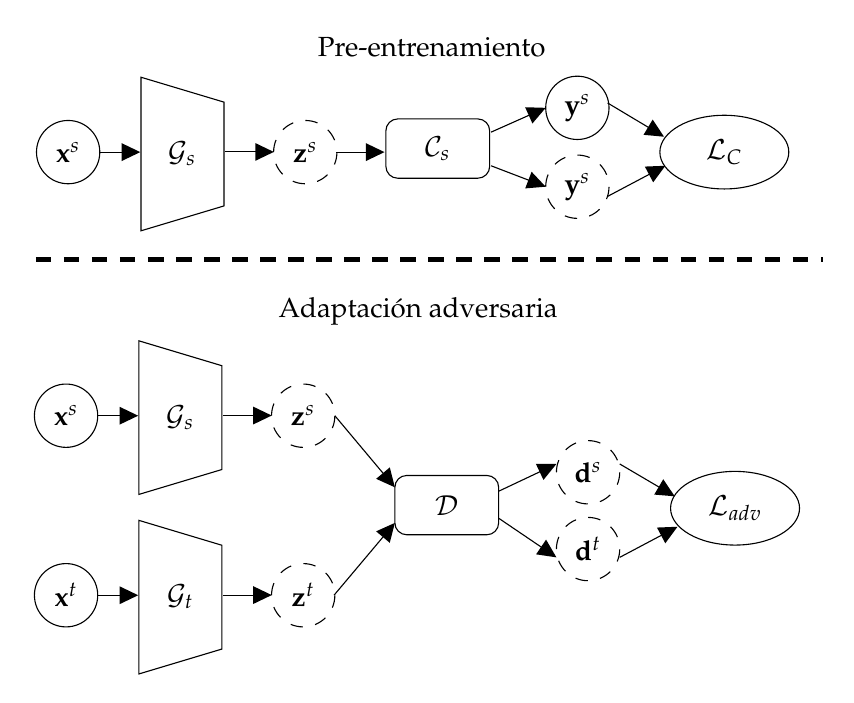
\begin{tikzpicture}[x=0.75pt,y=0.75pt,yscale=-1,xscale=1]
        %uncomment if require: \path (0,385); %set diagram left start at 0, and has height of 385

        \draw   (20.33,88.25) .. controls (20.33,79.83) and (27.16,73) .. (35.58,73) .. controls (44.01,73) and (50.83,79.83) .. (50.83,88.25) .. controls (50.83,96.67) and (44.01,103.5) .. (35.58,103.5) .. controls (27.16,103.5) and (20.33,96.67) .. (20.33,88.25) -- cycle ;

        \draw   (70.67,52.17) -- (110.67,64.17) -- (110.67,114.17) -- (70.67,126.17) -- cycle ;
        \draw    (50.83,88.25) -- (67.33,88.25) ;
        \draw [shift={(70.33,88.25)}, rotate = 180] [fill={rgb, 255:red, 0; green, 0; blue, 0 }  ][line width=0.08]  [draw opacity=0] (8.93,-4.29) -- (0,0) -- (8.93,4.29) -- cycle    ;
        \draw  [dash pattern={on 4.5pt off 4.5pt}] (134.58,88.25) .. controls (134.58,79.83) and (141.41,73) .. (149.83,73) .. controls (158.26,73) and (165.08,79.83) .. (165.08,88.25) .. controls (165.08,96.67) and (158.26,103.5) .. (149.83,103.5) .. controls (141.41,103.5) and (134.58,96.67) .. (134.58,88.25) -- cycle ;

        \draw   (188.67,77.98) .. controls (188.67,74.82) and (191.23,72.26) .. (194.38,72.26) -- (232.95,72.26) .. controls (236.11,72.26) and (238.67,74.82) .. (238.67,77.98) -- (238.67,95.12) .. controls (238.67,98.27) and (236.11,100.83) .. (232.95,100.83) -- (194.38,100.83) .. controls (191.23,100.83) and (188.67,98.27) .. (188.67,95.12) -- cycle ;
        \draw   (265.67,66.92) .. controls (265.67,58.49) and (272.49,51.67) .. (280.92,51.67) .. controls (289.34,51.67) and (296.17,58.49) .. (296.17,66.92) .. controls (296.17,75.34) and (289.34,82.17) .. (280.92,82.17) .. controls (272.49,82.17) and (265.67,75.34) .. (265.67,66.92) -- cycle ;
        \draw  [dash pattern={on 4.5pt off 4.5pt}] (265.67,104.92) .. controls (265.67,96.49) and (272.49,89.67) .. (280.92,89.67) .. controls (289.34,89.67) and (296.17,96.49) .. (296.17,104.92) .. controls (296.17,113.34) and (289.34,120.17) .. (280.92,120.17) .. controls (272.49,120.17) and (265.67,113.34) .. (265.67,104.92) -- cycle ;
        \draw   (320.67,88.25) .. controls (320.67,78.45) and (334.57,70.5) .. (351.73,70.5) .. controls (368.88,70.5) and (382.79,78.45) .. (382.79,88.25) .. controls (382.79,98.05) and (368.88,106) .. (351.73,106) .. controls (334.57,106) and (320.67,98.05) .. (320.67,88.25) -- cycle ;
        \draw    (111.33,88.17) -- (131.67,88.17) ;
        \draw [shift={(134.67,88.17)}, rotate = 180] [fill={rgb, 255:red, 0; green, 0; blue, 0 }  ][line width=0.08]  [draw opacity=0] (8.93,-4.29) -- (0,0) -- (8.93,4.29) -- cycle    ;
        \draw    (164.67,88.25) -- (185,88.25) ;
        \draw [shift={(188,88.25)}, rotate = 180] [fill={rgb, 255:red, 0; green, 0; blue, 0 }  ][line width=0.08]  [draw opacity=0] (8.93,-4.29) -- (0,0) -- (8.93,4.29) -- cycle    ;
        \draw    (239.33,78.64) -- (262.93,68.14) ;
        \draw [shift={(265.67,66.92)}, rotate = 156] [fill={rgb, 255:red, 0; green, 0; blue, 0 }  ][line width=0.08]  [draw opacity=0] (8.93,-4.29) -- (0,0) -- (8.93,4.29) -- cycle    ;
        \draw    (239.33,94.83) -- (262.87,103.84) ;
        \draw [shift={(265.67,104.92)}, rotate = 200.95] [fill={rgb, 255:red, 0; green, 0; blue, 0 }  ][line width=0.08]  [draw opacity=0] (8.93,-4.29) -- (0,0) -- (8.93,4.29) -- cycle    ;
        \draw    (295.5,64.58) -- (320.09,79.29) ;
        \draw [shift={(322.67,80.83)}, rotate = 210.89] [fill={rgb, 255:red, 0; green, 0; blue, 0 }  ][line width=0.08]  [draw opacity=0] (8.93,-4.29) -- (0,0) -- (8.93,4.29) -- cycle    ;
        \draw    (295.5,109.58) -- (320.68,96.24) ;
        \draw [shift={(323.33,94.83)}, rotate = 152.08] [fill={rgb, 255:red, 0; green, 0; blue, 0 }  ][line width=0.08]  [draw opacity=0] (8.93,-4.29) -- (0,0) -- (8.93,4.29) -- cycle    ;
        \draw   (19.33,215.25) .. controls (19.33,206.83) and (26.16,200) .. (34.58,200) .. controls (43.01,200) and (49.83,206.83) .. (49.83,215.25) .. controls (49.83,223.67) and (43.01,230.5) .. (34.58,230.5) .. controls (26.16,230.5) and (19.33,223.67) .. (19.33,215.25) -- cycle ;

        \draw   (69.67,179.17) -- (109.67,191.17) -- (109.67,241.17) -- (69.67,253.17) -- cycle ;
        \draw    (49.83,215.25) -- (66.33,215.25) ;
        \draw [shift={(69.33,215.25)}, rotate = 180] [fill={rgb, 255:red, 0; green, 0; blue, 0 }  ][line width=0.08]  [draw opacity=0] (8.93,-4.29) -- (0,0) -- (8.93,4.29) -- cycle    ;
        \draw  [dash pattern={on 4.5pt off 4.5pt}] (133.58,215.25) .. controls (133.58,206.83) and (140.41,200) .. (148.83,200) .. controls (157.26,200) and (164.08,206.83) .. (164.08,215.25) .. controls (164.08,223.67) and (157.26,230.5) .. (148.83,230.5) .. controls (140.41,230.5) and (133.58,223.67) .. (133.58,215.25) -- cycle ;

        \draw    (110.33,215.17) -- (130.67,215.17) ;
        \draw [shift={(133.67,215.17)}, rotate = 180] [fill={rgb, 255:red, 0; green, 0; blue, 0 }  ][line width=0.08]  [draw opacity=0] (8.93,-4.29) -- (0,0) -- (8.93,4.29) -- cycle    ;
        \draw    (164.08,215.25) -- (191.07,247.45) ;
        \draw [shift={(193,249.75)}, rotate = 230.03] [fill={rgb, 255:red, 0; green, 0; blue, 0 }  ][line width=0.08]  [draw opacity=0] (8.93,-4.29) -- (0,0) -- (8.93,4.29) -- cycle    ;
        \draw   (19.33,301.75) .. controls (19.33,293.33) and (26.16,286.5) .. (34.58,286.5) .. controls (43.01,286.5) and (49.83,293.33) .. (49.83,301.75) .. controls (49.83,310.17) and (43.01,317) .. (34.58,317) .. controls (26.16,317) and (19.33,310.17) .. (19.33,301.75) -- cycle ;

        \draw   (69.67,265.67) -- (109.67,277.67) -- (109.67,327.67) -- (69.67,339.67) -- cycle ;
        \draw    (49.83,301.75) -- (66.33,301.75) ;
        \draw [shift={(69.33,301.75)}, rotate = 180] [fill={rgb, 255:red, 0; green, 0; blue, 0 }  ][line width=0.08]  [draw opacity=0] (8.93,-4.29) -- (0,0) -- (8.93,4.29) -- cycle    ;
        \draw  [dash pattern={on 4.5pt off 4.5pt}] (133.58,301.75) .. controls (133.58,293.33) and (140.41,286.5) .. (148.83,286.5) .. controls (157.26,286.5) and (164.08,293.33) .. (164.08,301.75) .. controls (164.08,310.17) and (157.26,317) .. (148.83,317) .. controls (140.41,317) and (133.58,310.17) .. (133.58,301.75) -- cycle ;
        \draw    (110.33,301.67) -- (130.67,301.67) ;
        \draw [shift={(133.67,301.67)}, rotate = 180] [fill={rgb, 255:red, 0; green, 0; blue, 0 }  ][line width=0.08]  [draw opacity=0] (8.93,-4.29) -- (0,0) -- (8.93,4.29) -- cycle    ;
        \draw    (163.67,301.75) -- (191.07,269.19) ;
        \draw [shift={(193,266.89)}, rotate = 130.08] [fill={rgb, 255:red, 0; green, 0; blue, 0 }  ][line width=0.08]  [draw opacity=0] (8.93,-4.29) -- (0,0) -- (8.93,4.29) -- cycle    ;
        \draw   (193,249.75) .. controls (193,246.59) and (195.56,244.04) .. (198.71,244.04) -- (237.29,244.04) .. controls (240.44,244.04) and (243,246.59) .. (243,249.75) -- (243,266.89) .. controls (243,270.05) and (240.44,272.61) .. (237.29,272.61) -- (198.71,272.61) .. controls (195.56,272.61) and (193,270.05) .. (193,266.89) -- cycle ;

        \draw  [dash pattern={on 4.5pt off 4.5pt}] (270.83,242.5) .. controls (270.83,234.08) and (277.66,227.25) .. (286.08,227.25) .. controls (294.51,227.25) and (301.33,234.08) .. (301.33,242.5) .. controls (301.33,250.92) and (294.51,257.75) .. (286.08,257.75) .. controls (277.66,257.75) and (270.83,250.92) .. (270.83,242.5) -- cycle ;

        \draw  [dash pattern={on 4.5pt off 4.5pt}] (270.83,279.5) .. controls (270.83,271.08) and (277.66,264.25) .. (286.08,264.25) .. controls (294.51,264.25) and (301.33,271.08) .. (301.33,279.5) .. controls (301.33,287.92) and (294.51,294.75) .. (286.08,294.75) .. controls (277.66,294.75) and (270.83,287.92) .. (270.83,279.5) -- cycle ;

        \draw   (325.83,259.83) .. controls (325.83,250.03) and (339.74,242.08) .. (356.9,242.08) .. controls (374.05,242.08) and (387.96,250.03) .. (387.96,259.83) .. controls (387.96,269.64) and (374.05,277.58) .. (356.9,277.58) .. controls (339.74,277.58) and (325.83,269.64) .. (325.83,259.83) -- cycle ;

        \draw    (243.17,251.56) -- (268.12,239.78) ;
        \draw [shift={(270.83,238.5)}, rotate = 154.73] [fill={rgb, 255:red, 0; green, 0; blue, 0 }  ][line width=0.08]  [draw opacity=0] (8.93,-4.29) -- (0,0) -- (8.93,4.29) -- cycle    ;
        \draw    (243.17,264.75) -- (268.35,281.82) ;
        \draw [shift={(270.83,283.5)}, rotate = 214.13] [fill={rgb, 255:red, 0; green, 0; blue, 0 }  ][line width=0.08]  [draw opacity=0] (8.93,-4.29) -- (0,0) -- (8.93,4.29) -- cycle    ;
        \draw    (301.33,238.5) -- (325.25,252.56) ;
        \draw [shift={(327.83,254.08)}, rotate = 210.46] [fill={rgb, 255:red, 0; green, 0; blue, 0 }  ][line width=0.08]  [draw opacity=0] (8.93,-4.29) -- (0,0) -- (8.93,4.29) -- cycle    ;
        \draw    (301.33,283.5) -- (326.52,270.15) ;
        \draw [shift={(329.17,268.75)}, rotate = 152.08] [fill={rgb, 255:red, 0; green, 0; blue, 0 }  ][line width=0.08]  [draw opacity=0] (8.93,-4.29) -- (0,0) -- (8.93,4.29) -- cycle    ;
        \draw [line width=1.5]  [dash pattern={on 5.63pt off 4.5pt}]  (20,140) -- (399.5,140) ;

        \draw (280.92,66.92) node   [align=left] {\begin{minipage}[lt]{21.08pt}\setlength\topsep{0pt}
                \begin{center}
                    $\mathbf{y}^s$
                \end{center}
            \end{minipage}};
        \draw (280.92,104.92) node   [align=left] {\begin{minipage}[lt]{21.08pt}\setlength\topsep{0pt}
                \begin{center}
                    $\mathbf{y}^s$
                \end{center}
            \end{minipage}};
        \draw (351.73,88.25) node   [align=left] {\begin{minipage}[lt]{32.64pt}\setlength\topsep{0pt}
                \begin{center}
                    $\mathcal{L}_C$
                \end{center}
            \end{minipage}};
        \draw (149.83,88.25) node   [align=left] {\begin{minipage}[lt]{21.08pt}\setlength\topsep{0pt}
                \begin{center}
                    $\mathbf{z}^s$
                \end{center}
            \end{minipage}};
        \draw (35.58,88.25) node   [align=left] {\begin{minipage}[lt]{21.08pt}\setlength\topsep{0pt}
                \begin{center}
                    $\mathbf{x}^s$
                \end{center}
            \end{minipage}};
        \draw (90.67,89.17) node   [align=left] {\begin{minipage}[lt]{22.78pt}\setlength\topsep{0pt}
                \begin{center}
                    $\mathcal{G}_s$
                \end{center}
            \end{minipage}};
        \draw (213.67,86.73) node   [align=left] {\begin{minipage}[lt]{26.23pt}\setlength\topsep{0pt}
                \begin{center}
                    $\mathcal{C}_s$
                \end{center}
            \end{minipage}};
        \draw (89.67,216.17) node   [align=left] {\begin{minipage}[lt]{22.78pt}\setlength\topsep{0pt}
                \begin{center}
                    $\mathcal{G}_s$
                \end{center}
            \end{minipage}};
        \draw (148.83,215.25) node   [align=left] {\begin{minipage}[lt]{21.08pt}\setlength\topsep{0pt}
                \begin{center}
                    $\mathbf{z}^s$
                \end{center}
            \end{minipage}};
        \draw (34.58,215.25) node   [align=left] {\begin{minipage}[lt]{21.08pt}\setlength\topsep{0pt}
                \begin{center}
                    $\mathbf{x}^s$
                \end{center}
            \end{minipage}};
        \draw (89.67,302.67) node   [align=left] {\begin{minipage}[lt]{22.78pt}\setlength\topsep{0pt}
                \begin{center}
                    $\mathcal{G}_t$
                \end{center}
            \end{minipage}};
        \draw (34.58,301.75) node   [align=left] {\begin{minipage}[lt]{21.08pt}\setlength\topsep{0pt}
                \begin{center}
                    $\mathbf{x}^t$
                \end{center}
            \end{minipage}};
        \draw (148.83,301.75) node   [align=left] {\begin{minipage}[lt]{21.08pt}\setlength\topsep{0pt}
                \begin{center}
                    $\mathbf{z}^t$
                \end{center}
            \end{minipage}};
        \draw (218,258.5) node   [align=left] {\begin{minipage}[lt]{26.23pt}\setlength\topsep{0pt}
                \begin{center}
                    $\mathcal{D}$
                \end{center}
            \end{minipage}};
        \draw (356.9,259.83) node   [align=left] {\begin{minipage}[lt]{32.64pt}\setlength\topsep{0pt}
                \begin{center}
                    $\mathcal{L}_{adv}$
                \end{center}
            \end{minipage}};
        \draw (286.08,279.5) node   [align=left] {\begin{minipage}[lt]{21.08pt}\setlength\topsep{0pt}
                \begin{center}
                    $\mathbf{d}^t$
                \end{center}
            \end{minipage}};
        \draw (286.08,242.5) node   [align=left] {\begin{minipage}[lt]{21.08pt}\setlength\topsep{0pt}
                \begin{center}
                    $\mathbf{d}^s$
                \end{center}
            \end{minipage}};
        \draw (210.75,37.5) node   [align=left] {\begin{minipage}[lt]{258.06pt}\setlength\topsep{0pt}
                \begin{center}
                    Pre-entrenamiento
                \end{center}
            \end{minipage}};
        \draw (204.25,165) node   [align=left] {\begin{minipage}[lt]{266.22pt}\setlength\topsep{0pt}
                \begin{center}
                    Adaptaci\'on adversaria
                \end{center}
            \end{minipage}};

    \end{tikzpicture}
    \caption{Esquema de las {\it ADDA}. Los supra indices $s$ y $t$ indican si los datos son del origen o destino respectivamente.
        Los c\'irculos con l\'ineas rayadas son salidas de los modelos mientras que los c\'irculos de l\'ineas s\'olidas son datos conocidos.
        La primera fase consta de un pre-entrenamiento con una red generadora $\mathcal{G}_s$ con los datos origen y la segunda fase de adaptaci\'on
        consta de otra red generadora $\mathcal{G}_t$ que debe aprender a generar el mismo espacio latente que $\mathcal{G}_s$ con los datos de destino para confundir a $\mathcal{D}$.}
    \label{fig:adda-esquema}
\end{figure}

No obstante del cambio, los objetivos son similares a {\it ADDA} excepci\'on de $\mathcal{G}_t$. La ecuaci\'on
\ref{eq:adda-loss-clasificadora} contiene $\mathcal{L}_\mathcal{C}$ que es an\'aloga a
\ref{eq:dann-loss-clasificadora}. La ecuaci\'on \ref{eq:adda-loss-discriminadora} contiene $\mathcal{L}_{adv}$ que es
an\'aloga a \ref{eq:dann-loss-discriminadora}. Finalmente, la ecuaci\'on \ref{eq:adda-objetivo} contiene el objetivo a
optimizar que asigna gradientes peque\~{n}os a registros de destino que sean similares a los de origen y gradientes mas
grandes para los otros registros de destino.

\begin{align}
     & \min_{\mathcal{G}_s, \mathcal{C}} \mathcal{L}_\mathcal{C}(\mathbf{x}^s, \mathbf{y}^s)                                                            = \mathcal{L}_{CE}(C_s(\mathcal{G}_s(\mathbf{x}^s)), \mathbf{y}^s)
    \label{eq:adda-loss-clasificadora}                                                                                                                                                                                                                                                                                                                                                          \\
     & \max_{\mathcal{D}} \mathcal{L}_{adv}(\mathbf{x}^s, \mathbf{x}^t)                                                                                 = \mathbb{E}_{\mathbf{x}^s \sim \mathcal{\hat{S}}}\log[\mathcal{D}(\mathcal{G}_s(\mathbf{x}^s))] + \mathbb{E}_{\mathbf{x}^t \sim \mathcal{\hat{T}}}\log[1-\mathcal{D}(\mathcal{G}_t(\mathbf{x}^t))] \label{eq:adda-loss-discriminadora} \\
     & \min_{\mathcal{G}_t} - \mathbb{E}_{\mathbf{x}^t \sim \mathcal{\hat{T}}} \log[\mathcal{D}(\mathcal{G}_t(\mathbf{x}^t))]  \label{eq:adda-objetivo}
\end{align}

\subsection{Batch Spectral Penalization}

Aunque los metodos de adaptaci\'on de dominio adversarios mejoran la {\it transferibilidad} de las características
aprendidas; es decir, la capacidad de que las representaciones puedan superar las discrepancias entre los dominios, lo
hacen a costa de la {\it discriminabilidad}; es decir, la facilidad de separar categorias sobre las representaciones de
ambos dominios \parencite{chen2019transferability}. Al aplicar descomposici\'on en valores singulares ({\it SVD} en ingl\'es) para
analizar las propiedades espectrales de las representaciones aprendidas en batches, se confirma que los eigenvectors
con valores singulares m\'as altos dominan la {\it transferibilidad} mientras que los eigenvectors con valores
singulares m\'as pequeños se encuentran penalizados lo que provoca una {\it discriminabilidad} deficiente. {\it Batch
        Spectral Penalization} {\it BSP} \parencite{chen2019transferability} penaliza el mayor valor singular para que los dem\'as eigenvectors puedan mejorar la
    {\it discriminabilidad}. $\mathcal{L}_{BSP}$ es propuesto como un t\'ermino de regularizaci\'on sobre los $k$ mayores
valores singulares:

\begin{align}
    \mathcal{L}_{BSP}(\mathbf{z}) = \sum_{i=0}^{k} (\sigma_{s, i}^2 + \sigma_{t, i}^2)
    \label{eq:bsp}
\end{align}

Donde $\sigma_{s, i}$ y $\sigma_{t, i}$ corresponden al $i$-\'esimo mayor valor singular de $\Sigma_s$ y $\Sigma_t$
respectivamente. En la presente tesis se utilizar\'a $k=1$.

    {\it BSP} puede integrarse a cualquiera de los esquemas mencionados anteriormente, por ejemplo a una {\it DANN} (figura \ref{fig:bsp-esquema-dann}).

\begin{figure}[H]
    \centering

    \tikzset{every picture/.style={line width=0.75pt}} %set default line width to 0.75pt        

    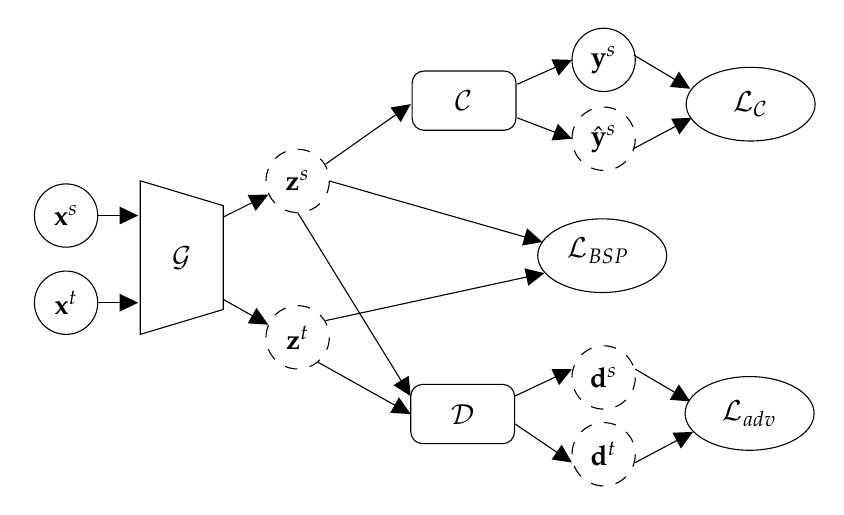
\begin{tikzpicture}[x=0.75pt,y=0.75pt,yscale=-1,xscale=1]
        %uncomment if require: \path (0,300); %set diagram left start at 0, and has height of 300

        %Shape: Circle [id:dp14395415737572304] 
        \draw   (57,126.75) .. controls (57,118.33) and (63.83,111.5) .. (72.25,111.5) .. controls (80.67,111.5) and (87.5,118.33) .. (87.5,126.75) .. controls (87.5,135.17) and (80.67,142) .. (72.25,142) .. controls (63.83,142) and (57,135.17) .. (57,126.75) -- cycle ;

        %Shape: Circle [id:dp5294927781460403] 
        \draw   (57,168.75) .. controls (57,160.33) and (63.83,153.5) .. (72.25,153.5) .. controls (80.67,153.5) and (87.5,160.33) .. (87.5,168.75) .. controls (87.5,177.17) and (80.67,184) .. (72.25,184) .. controls (63.83,184) and (57,177.17) .. (57,168.75) -- cycle ;

        %Shape: Trapezoid [id:dp3621515034386269] 
        \draw   (108,110) -- (148,122) -- (148,172) -- (108,184) -- cycle ;

        %Straight Lines [id:da711615291035981] 
        \draw    (87.5,126.75) -- (104,126.75) ;
        \draw [shift={(107,126.75)}, rotate = 180] [fill={rgb, 255:red, 0; green, 0; blue, 0 }  ][line width=0.08]  [draw opacity=0] (8.93,-4.29) -- (0,0) -- (8.93,4.29) -- cycle    ;
        %Shape: Circle [id:dp5854711906138592] 
        \draw  [dash pattern={on 4.5pt off 4.5pt}] (168.58,110.08) .. controls (168.58,101.66) and (175.41,94.83) .. (183.83,94.83) .. controls (192.26,94.83) and (199.08,101.66) .. (199.08,110.08) .. controls (199.08,118.51) and (192.26,125.33) .. (183.83,125.33) .. controls (175.41,125.33) and (168.58,118.51) .. (168.58,110.08) -- cycle ;

        %Shape: Circle [id:dp8402316163188099] 
        \draw  [dash pattern={on 4.5pt off 4.5pt}] (168.58,185.42) .. controls (168.58,176.99) and (175.41,170.17) .. (183.83,170.17) .. controls (192.26,170.17) and (199.08,176.99) .. (199.08,185.42) .. controls (199.08,193.84) and (192.26,200.67) .. (183.83,200.67) .. controls (175.41,200.67) and (168.58,193.84) .. (168.58,185.42) -- cycle ;

        %Rounded Rect [id:dp15165955457538138] 
        \draw   (239,62.81) .. controls (239,59.65) and (241.56,57.1) .. (244.71,57.1) -- (283.29,57.1) .. controls (286.44,57.1) and (289,59.65) .. (289,62.81) -- (289,79.95) .. controls (289,83.11) and (286.44,85.67) .. (283.29,85.67) -- (244.71,85.67) .. controls (241.56,85.67) and (239,83.11) .. (239,79.95) -- cycle ;

        %Rounded Rect [id:dp47289041628378614] 
        \draw   (238.33,213.81) .. controls (238.33,210.65) and (240.89,208.1) .. (244.05,208.1) -- (282.62,208.1) .. controls (285.77,208.1) and (288.33,210.65) .. (288.33,213.81) -- (288.33,230.95) .. controls (288.33,234.11) and (285.77,236.67) .. (282.62,236.67) -- (244.05,236.67) .. controls (240.89,236.67) and (238.33,234.11) .. (238.33,230.95) -- cycle ;

        %Shape: Circle [id:dp20484409800302994] 
        \draw  [dash pattern={on 4.5pt off 4.5pt}] (316,204.75) .. controls (316,196.33) and (322.83,189.5) .. (331.25,189.5) .. controls (339.67,189.5) and (346.5,196.33) .. (346.5,204.75) .. controls (346.5,213.17) and (339.67,220) .. (331.25,220) .. controls (322.83,220) and (316,213.17) .. (316,204.75) -- cycle ;

        %Shape: Circle [id:dp19954579063976796] 
        \draw  [dash pattern={on 4.5pt off 4.5pt}] (316,241.75) .. controls (316,233.33) and (322.83,226.5) .. (331.25,226.5) .. controls (339.67,226.5) and (346.5,233.33) .. (346.5,241.75) .. controls (346.5,250.17) and (339.67,257) .. (331.25,257) .. controls (322.83,257) and (316,250.17) .. (316,241.75) -- cycle ;

        %Shape: Ellipse [id:dp41632665310072503] 
        \draw   (370.5,222.08) .. controls (370.5,212.28) and (384.41,204.33) .. (401.56,204.33) .. controls (418.72,204.33) and (432.63,212.28) .. (432.63,222.08) .. controls (432.63,231.89) and (418.72,239.83) .. (401.56,239.83) .. controls (384.41,239.83) and (370.5,231.89) .. (370.5,222.08) -- cycle ;

        %Shape: Circle [id:dp17102829278099274] 
        \draw   (316,51.75) .. controls (316,43.33) and (322.83,36.5) .. (331.25,36.5) .. controls (339.67,36.5) and (346.5,43.33) .. (346.5,51.75) .. controls (346.5,60.17) and (339.67,67) .. (331.25,67) .. controls (322.83,67) and (316,60.17) .. (316,51.75) -- cycle ;
        %Shape: Circle [id:dp2918994940011912] 
        \draw  [dash pattern={on 4.5pt off 4.5pt}] (316,89.75) .. controls (316,81.33) and (322.83,74.5) .. (331.25,74.5) .. controls (339.67,74.5) and (346.5,81.33) .. (346.5,89.75) .. controls (346.5,98.17) and (339.67,105) .. (331.25,105) .. controls (322.83,105) and (316,98.17) .. (316,89.75) -- cycle ;
        %Shape: Ellipse [id:dp7208514036481783] 
        \draw   (371,73.08) .. controls (371,63.28) and (384.91,55.33) .. (402.06,55.33) .. controls (419.22,55.33) and (433.13,63.28) .. (433.13,73.08) .. controls (433.13,82.89) and (419.22,90.83) .. (402.06,90.83) .. controls (384.91,90.83) and (371,82.89) .. (371,73.08) -- cycle ;
        %Straight Lines [id:da35699780719749463] 
        \draw    (87.5,168.75) -- (104,168.75) ;
        \draw [shift={(107,168.75)}, rotate = 180] [fill={rgb, 255:red, 0; green, 0; blue, 0 }  ][line width=0.08]  [draw opacity=0] (8.93,-4.29) -- (0,0) -- (8.93,4.29) -- cycle    ;
        %Straight Lines [id:da18773339124658595] 
        \draw    (148.33,127.33) -- (166.98,118.01) ;
        \draw [shift={(169.67,116.67)}, rotate = 153.43] [fill={rgb, 255:red, 0; green, 0; blue, 0 }  ][line width=0.08]  [draw opacity=0] (8.93,-4.29) -- (0,0) -- (8.93,4.29) -- cycle    ;
        %Straight Lines [id:da22178069673434142] 
        \draw    (148.33,167.33) -- (167.05,177.86) ;
        \draw [shift={(169.67,179.33)}, rotate = 209.36] [fill={rgb, 255:red, 0; green, 0; blue, 0 }  ][line width=0.08]  [draw opacity=0] (8.93,-4.29) -- (0,0) -- (8.93,4.29) -- cycle    ;
        %Straight Lines [id:da7263329854343115] 
        \draw    (197.25,102) -- (235.88,74.81) ;
        \draw [shift={(238.33,73.08)}, rotate = 144.86] [fill={rgb, 255:red, 0; green, 0; blue, 0 }  ][line width=0.08]  [draw opacity=0] (8.93,-4.29) -- (0,0) -- (8.93,4.29) -- cycle    ;
        %Straight Lines [id:da5895896069004276] 
        \draw    (193.6,197.4) -- (235.71,220.95) ;
        \draw [shift={(238.33,222.42)}, rotate = 209.22] [fill={rgb, 255:red, 0; green, 0; blue, 0 }  ][line width=0.08]  [draw opacity=0] (8.93,-4.29) -- (0,0) -- (8.93,4.29) -- cycle    ;
        %Straight Lines [id:da504234275800213] 
        \draw    (183.83,125.33) -- (236.76,211.26) ;
        \draw [shift={(238.33,213.81)}, rotate = 238.37] [fill={rgb, 255:red, 0; green, 0; blue, 0 }  ][line width=0.08]  [draw opacity=0] (8.93,-4.29) -- (0,0) -- (8.93,4.29) -- cycle    ;
        %Straight Lines [id:da10127819240633107] 
        \draw    (288.33,213.81) -- (313.29,202.03) ;
        \draw [shift={(316,200.75)}, rotate = 154.73] [fill={rgb, 255:red, 0; green, 0; blue, 0 }  ][line width=0.08]  [draw opacity=0] (8.93,-4.29) -- (0,0) -- (8.93,4.29) -- cycle    ;
        %Straight Lines [id:da18118282714853473] 
        \draw    (288.33,227) -- (313.52,244.07) ;
        \draw [shift={(316,245.75)}, rotate = 214.13] [fill={rgb, 255:red, 0; green, 0; blue, 0 }  ][line width=0.08]  [draw opacity=0] (8.93,-4.29) -- (0,0) -- (8.93,4.29) -- cycle    ;
        %Straight Lines [id:da46435990995985477] 
        \draw    (346.5,200.75) -- (370.41,214.81) ;
        \draw [shift={(373,216.33)}, rotate = 210.46] [fill={rgb, 255:red, 0; green, 0; blue, 0 }  ][line width=0.08]  [draw opacity=0] (8.93,-4.29) -- (0,0) -- (8.93,4.29) -- cycle    ;
        %Straight Lines [id:da3066500527802958] 
        \draw    (346.5,245.75) -- (371.68,232.4) ;
        \draw [shift={(374.33,231)}, rotate = 152.08] [fill={rgb, 255:red, 0; green, 0; blue, 0 }  ][line width=0.08]  [draw opacity=0] (8.93,-4.29) -- (0,0) -- (8.93,4.29) -- cycle    ;
        %Straight Lines [id:da9357957653419868] 
        \draw    (289.67,63.48) -- (313.26,52.97) ;
        \draw [shift={(316,51.75)}, rotate = 156] [fill={rgb, 255:red, 0; green, 0; blue, 0 }  ][line width=0.08]  [draw opacity=0] (8.93,-4.29) -- (0,0) -- (8.93,4.29) -- cycle    ;
        %Straight Lines [id:da5822336916421971] 
        \draw    (289.67,79.67) -- (313.2,88.68) ;
        \draw [shift={(316,89.75)}, rotate = 200.95] [fill={rgb, 255:red, 0; green, 0; blue, 0 }  ][line width=0.08]  [draw opacity=0] (8.93,-4.29) -- (0,0) -- (8.93,4.29) -- cycle    ;
        %Straight Lines [id:da8400721166176619] 
        \draw    (345.83,49.42) -- (370.43,64.13) ;
        \draw [shift={(373,65.67)}, rotate = 210.89] [fill={rgb, 255:red, 0; green, 0; blue, 0 }  ][line width=0.08]  [draw opacity=0] (8.93,-4.29) -- (0,0) -- (8.93,4.29) -- cycle    ;
        %Straight Lines [id:da5048948243554285] 
        \draw    (345.83,94.42) -- (371.02,81.07) ;
        \draw [shift={(373.67,79.67)}, rotate = 152.08] [fill={rgb, 255:red, 0; green, 0; blue, 0 }  ][line width=0.08]  [draw opacity=0] (8.93,-4.29) -- (0,0) -- (8.93,4.29) -- cycle    ;
        %Shape: Ellipse [id:dp8464659325338855] 
        \draw   (299.5,146.08) .. controls (299.5,136.28) and (313.41,128.33) .. (330.56,128.33) .. controls (347.72,128.33) and (361.63,136.28) .. (361.63,146.08) .. controls (361.63,155.89) and (347.72,163.83) .. (330.56,163.83) .. controls (313.41,163.83) and (299.5,155.89) .. (299.5,146.08) -- cycle ;
        %Straight Lines [id:da5523565128759309] 
        \draw    (197.2,177.4) -- (299.82,155.14) ;
        \draw [shift={(302.75,154.5)}, rotate = 167.76] [fill={rgb, 255:red, 0; green, 0; blue, 0 }  ][line width=0.08]  [draw opacity=0] (8.93,-4.29) -- (0,0) -- (8.93,4.29) -- cycle    ;
        %Straight Lines [id:da24838256047555873] 
        \draw    (199.08,110.08) -- (298.87,138.67) ;
        \draw [shift={(301.75,139.5)}, rotate = 195.99] [fill={rgb, 255:red, 0; green, 0; blue, 0 }  ][line width=0.08]  [draw opacity=0] (8.93,-4.29) -- (0,0) -- (8.93,4.29) -- cycle    ;

        % Text Node
        \draw (331.25,51.75) node   [align=left] {\begin{minipage}[lt]{21.08pt}\setlength\topsep{0pt}
                \begin{center}
                    $\mathbf{y}^s$
                \end{center}

            \end{minipage}};
        % Text Node
        \draw (331.25,89.75) node   [align=left] {\begin{minipage}[lt]{21.08pt}\setlength\topsep{0pt}
                \begin{center}
                    $\hat{\mathbf{y}}^s$
                \end{center}

            \end{minipage}};
        % Text Node
        \draw (402.06,73.08) node   [align=left] {\begin{minipage}[lt]{32.64pt}\setlength\topsep{0pt}
                \begin{center}
                    $\mathcal{L}_{\mathcal{C}}$
                \end{center}

            \end{minipage}};
        % Text Node
        \draw (401.56,222.08) node   [align=left] {\begin{minipage}[lt]{32.64pt}\setlength\topsep{0pt}
                \begin{center}
                    $\mathcal{L}_{adv}$
                \end{center}

            \end{minipage}};
        % Text Node
        \draw (331.25,241.75) node   [align=left] {\begin{minipage}[lt]{21.08pt}\setlength\topsep{0pt}
                \begin{center}
                    $\mathbf{d}^t$
                \end{center}

            \end{minipage}};
        % Text Node
        \draw (331.25,204.75) node   [align=left] {\begin{minipage}[lt]{21.08pt}\setlength\topsep{0pt}
                \begin{center}
                    $\mathbf{d}^s$
                \end{center}

            \end{minipage}};
        % Text Node
        \draw (263.33,222.56) node   [align=left] {\begin{minipage}[lt]{26.23pt}\setlength\topsep{0pt}
                \begin{center}
                    $\mathcal{D}$
                \end{center}

            \end{minipage}};
        % Text Node
        \draw (264,71.56) node   [align=left] {\begin{minipage}[lt]{26.23pt}\setlength\topsep{0pt}
                \begin{center}
                    $\mathcal{C}$
                \end{center}

            \end{minipage}};
        % Text Node
        \draw (183.83,185.42) node   [align=left] {\begin{minipage}[lt]{21.08pt}\setlength\topsep{0pt}
                \begin{center}
                    $\mathbf{z}^t$
                \end{center}

            \end{minipage}};
        % Text Node
        \draw (183.83,110.08) node   [align=left] {\begin{minipage}[lt]{21.08pt}\setlength\topsep{0pt}
                \begin{center}
                    $\mathbf{z}^s$
                \end{center}

            \end{minipage}};
        % Text Node
        \draw (128,147) node   [align=left] {\begin{minipage}[lt]{22.78pt}\setlength\topsep{0pt}
                \begin{center}
                    $\mathcal{G}$
                \end{center}

            \end{minipage}};
        % Text Node
        \draw (72.25,168.75) node   [align=left] {\begin{minipage}[lt]{21.08pt}\setlength\topsep{0pt}
                \begin{center}
                    $\mathbf{x}^t$
                \end{center}

            \end{minipage}};
        % Text Node
        \draw (72.25,126.75) node   [align=left] {\begin{minipage}[lt]{21.08pt}\setlength\topsep{0pt}
                \begin{center}
                    $\mathbf{x}^s$
                \end{center}

            \end{minipage}};
        % Text Node
        \draw (312.5,136.4) node [anchor=north west][inner sep=0.75pt]    {$\mathcal{L}_{BSP} $};

    \end{tikzpicture}

    \caption{Esquema de un modelo {\it DANN+BSP}.}
    \label{fig:bsp-esquema-dann}
\end{figure}

Por lo tanto, un modelo {\it DANN+BSP} presenta como objetivos:

\begin{align}
     & \min_{\mathcal{G},\mathcal{C}} \mathcal{L}_\mathcal{C}(\mathbf{x}^s, \mathbf{y}^s) + \lambda \mathcal{L}_{adv}(\mathbf{x}^s, \mathbf{x}^t) + \beta \mathcal{L}_{BSP}(\mathcal{G}(\mathbf{x})) \\
     & \max_{\mathcal{D}} \mathcal{L}_{adv}(\mathbf{x}^s, \mathbf{x}^t)
    \label{eq:bsp-dann-obejtivo}
\end{align}

Donde $\beta$ es el par\'ametro que regula el trade-off de $\mathcal{L}_{BSP}$.

\subsection{Margin Disparity Discrepancy}

Las t\'ecnicas detalladas hasta el momento implican algoritmos de optimizaci\'on minimax, que funcionan correctamente
en los m\'etodos basados en el aprendizaje adversario. Sin embargo, estos algoritmos utilizan funciones de scoreoque
carecen de garant\'ias te\'oricas ya que se estudiaron funciones de p\'erdida 0-1. Es por esto que se introducen
m\'etodos que apuntan a reducir la brecha que existe entre la teor\'ia y el algoritmo, como Margin Disparity
Discrepancy {\it MDD} \parencite{zhang2019bridging}.

\begin{figure}[H]
    \centering

    \tikzset{every picture/.style={line width=0.75pt}} %set default line width to 0.75pt        

    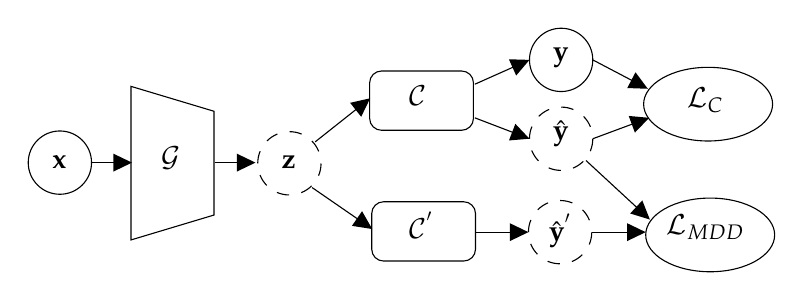
\begin{tikzpicture}[x=0.75pt,y=0.75pt,yscale=-1,xscale=1]
        %uncomment if require: \path (0,424); %set diagram left start at 0, and has height of 424

        %Shape: Circle [id:dp37402229817841603] 
        \draw   (60.5,104.75) .. controls (60.5,96.33) and (67.33,89.5) .. (75.75,89.5) .. controls (84.17,89.5) and (91,96.33) .. (91,104.75) .. controls (91,113.17) and (84.17,120) .. (75.75,120) .. controls (67.33,120) and (60.5,113.17) .. (60.5,104.75) -- cycle ;
        %Shape: Trapezoid [id:dp5518581764728496] 
        \draw   (110,68) -- (150,80) -- (150,130) -- (110,142) -- cycle ;
        %Straight Lines [id:da7900111351501842] 
        \draw    (91,104.75) -- (107.5,104.75) ;
        \draw [shift={(110.5,104.75)}, rotate = 180] [fill={rgb, 255:red, 0; green, 0; blue, 0 }  ][line width=0.08]  [draw opacity=0] (8.93,-4.29) -- (0,0) -- (8.93,4.29) -- cycle    ;
        %Shape: Circle [id:dp6237032464701955] 
        \draw  [dash pattern={on 4.5pt off 4.5pt}] (171.08,105.08) .. controls (171.08,96.66) and (177.91,89.83) .. (186.33,89.83) .. controls (194.76,89.83) and (201.58,96.66) .. (201.58,105.08) .. controls (201.58,113.51) and (194.76,120.33) .. (186.33,120.33) .. controls (177.91,120.33) and (171.08,113.51) .. (171.08,105.08) -- cycle ;
        %Rounded Rect [id:dp17455651105714143] 
        \draw   (225,66.31) .. controls (225,63.15) and (227.56,60.6) .. (230.71,60.6) -- (269.29,60.6) .. controls (272.44,60.6) and (275,63.15) .. (275,66.31) -- (275,83.45) .. controls (275,86.61) and (272.44,89.17) .. (269.29,89.17) -- (230.71,89.17) .. controls (227.56,89.17) and (225,86.61) .. (225,83.45) -- cycle ;
        %Shape: Circle [id:dp2140151642409336] 
        \draw   (302,55.25) .. controls (302,46.83) and (308.83,40) .. (317.25,40) .. controls (325.67,40) and (332.5,46.83) .. (332.5,55.25) .. controls (332.5,63.67) and (325.67,70.5) .. (317.25,70.5) .. controls (308.83,70.5) and (302,63.67) .. (302,55.25) -- cycle ;
        %Shape: Circle [id:dp8313620493224034] 
        \draw  [dash pattern={on 4.5pt off 4.5pt}] (302,93.25) .. controls (302,84.83) and (308.83,78) .. (317.25,78) .. controls (325.67,78) and (332.5,84.83) .. (332.5,93.25) .. controls (332.5,101.67) and (325.67,108.5) .. (317.25,108.5) .. controls (308.83,108.5) and (302,101.67) .. (302,93.25) -- cycle ;
        %Shape: Ellipse [id:dp0600451143745524] 
        \draw   (357,76.58) .. controls (357,66.78) and (370.91,58.83) .. (388.06,58.83) .. controls (405.22,58.83) and (419.13,66.78) .. (419.13,76.58) .. controls (419.13,86.39) and (405.22,94.33) .. (388.06,94.33) .. controls (370.91,94.33) and (357,86.39) .. (357,76.58) -- cycle ;
        %Straight Lines [id:da9980456278456524] 
        \draw    (198.75,94.75) -- (222.9,75.61) ;
        \draw [shift={(225.25,73.75)}, rotate = 141.6] [fill={rgb, 255:red, 0; green, 0; blue, 0 }  ][line width=0.08]  [draw opacity=0] (8.93,-4.29) -- (0,0) -- (8.93,4.29) -- cycle    ;
        %Straight Lines [id:da3629940013678272] 
        \draw    (275.67,66.98) -- (299.26,56.47) ;
        \draw [shift={(302,55.25)}, rotate = 156] [fill={rgb, 255:red, 0; green, 0; blue, 0 }  ][line width=0.08]  [draw opacity=0] (8.93,-4.29) -- (0,0) -- (8.93,4.29) -- cycle    ;
        %Straight Lines [id:da8352907095901936] 
        \draw    (275.67,83.17) -- (299.2,92.18) ;
        \draw [shift={(302,93.25)}, rotate = 200.95] [fill={rgb, 255:red, 0; green, 0; blue, 0 }  ][line width=0.08]  [draw opacity=0] (8.93,-4.29) -- (0,0) -- (8.93,4.29) -- cycle    ;
        %Straight Lines [id:da1138581727231831] 
        \draw    (332.5,55.25) -- (356.34,67.77) ;
        \draw [shift={(359,69.17)}, rotate = 207.71] [fill={rgb, 255:red, 0; green, 0; blue, 0 }  ][line width=0.08]  [draw opacity=0] (8.93,-4.29) -- (0,0) -- (8.93,4.29) -- cycle    ;
        %Straight Lines [id:da07484994635417963] 
        \draw    (332.5,93.25) -- (356.85,84.21) ;
        \draw [shift={(359.67,83.17)}, rotate = 159.64] [fill={rgb, 255:red, 0; green, 0; blue, 0 }  ][line width=0.08]  [draw opacity=0] (8.93,-4.29) -- (0,0) -- (8.93,4.29) -- cycle    ;
        %Straight Lines [id:da7386987904124067] 
        \draw    (150.5,104.75) -- (167,104.75) ;
        \draw [shift={(170,104.75)}, rotate = 180] [fill={rgb, 255:red, 0; green, 0; blue, 0 }  ][line width=0.08]  [draw opacity=0] (8.93,-4.29) -- (0,0) -- (8.93,4.29) -- cycle    ;
        %Rounded Rect [id:dp7058372380502067] 
        \draw   (226,129.31) .. controls (226,126.15) and (228.56,123.6) .. (231.71,123.6) -- (270.29,123.6) .. controls (273.44,123.6) and (276,126.15) .. (276,129.31) -- (276,146.45) .. controls (276,149.61) and (273.44,152.17) .. (270.29,152.17) -- (231.71,152.17) .. controls (228.56,152.17) and (226,149.61) .. (226,146.45) -- cycle ;
        %Shape: Circle [id:dp8799954567091415] 
        \draw  [dash pattern={on 4.5pt off 4.5pt}] (301.5,138.25) .. controls (301.5,129.83) and (308.33,123) .. (316.75,123) .. controls (325.17,123) and (332,129.83) .. (332,138.25) .. controls (332,146.67) and (325.17,153.5) .. (316.75,153.5) .. controls (308.33,153.5) and (301.5,146.67) .. (301.5,138.25) -- cycle ;
        %Shape: Ellipse [id:dp09534345336772221] 
        \draw   (358,139.58) .. controls (358,129.78) and (371.91,121.83) .. (389.06,121.83) .. controls (406.22,121.83) and (420.13,129.78) .. (420.13,139.58) .. controls (420.13,149.39) and (406.22,157.33) .. (389.06,157.33) .. controls (371.91,157.33) and (358,149.39) .. (358,139.58) -- cycle ;
        %Straight Lines [id:da6601974145410334] 
        \draw    (197.25,116.75) -- (223.78,135.05) ;
        \draw [shift={(226.25,136.75)}, rotate = 214.59] [fill={rgb, 255:red, 0; green, 0; blue, 0 }  ][line width=0.08]  [draw opacity=0] (8.93,-4.29) -- (0,0) -- (8.93,4.29) -- cycle    ;
        %Straight Lines [id:da32804094797701633] 
        \draw    (275.75,138.25) -- (298.5,138.25) ;
        \draw [shift={(301.5,138.25)}, rotate = 180] [fill={rgb, 255:red, 0; green, 0; blue, 0 }  ][line width=0.08]  [draw opacity=0] (8.93,-4.29) -- (0,0) -- (8.93,4.29) -- cycle    ;
        %Straight Lines [id:da19377630354971975] 
        \draw    (329.25,103.75) -- (357.8,130.13) ;
        \draw [shift={(360,132.17)}, rotate = 222.74] [fill={rgb, 255:red, 0; green, 0; blue, 0 }  ][line width=0.08]  [draw opacity=0] (8.93,-4.29) -- (0,0) -- (8.93,4.29) -- cycle    ;
        %Straight Lines [id:da39400351361192065] 
        \draw    (332,138.25) -- (355,138.25) ;
        \draw [shift={(358,138.25)}, rotate = 180] [fill={rgb, 255:red, 0; green, 0; blue, 0 }  ][line width=0.08]  [draw opacity=0] (8.93,-4.29) -- (0,0) -- (8.93,4.29) -- cycle    ;

        % Text Node
        \draw (70.67,100) node [anchor=north west][inner sep=0.75pt]    {$\mathbf{x}$};
        % Text Node
        \draw (123.33,95.73) node [anchor=north west][inner sep=0.75pt]    {$\mathcal{G}$};
        % Text Node
        \draw (181.33,100) node [anchor=north west][inner sep=0.75pt]    {$\mathbf{z}$};
        % Text Node
        \draw (242.67,66.4) node [anchor=north west][inner sep=0.75pt]    {$\mathcal{C}$};
        % Text Node
        \draw (242.67,127) node [anchor=north west][inner sep=0.75pt]    {$\mathcal{C}^{'}$};
        % Text Node
        \draw (310,128) node [anchor=north west][inner sep=0.75pt]    {$\hat{\mathbf{y}}^{'}$};
        % Text Node
        \draw (312,83.4) node [anchor=north west][inner sep=0.75pt]    {$\hat{\mathbf{y}}$};
        % Text Node
        \draw (312,48) node [anchor=north west][inner sep=0.75pt]    {$\mathbf{y}$};
        % Text Node
        \draw (376.67,67.4) node [anchor=north west][inner sep=0.75pt]    {$\mathcal{L}_{C}$};
        % Text Node
        \draw (366.67,128.73) node [anchor=north west][inner sep=0.75pt]    {$\mathcal{L}_{MDD}$};

    \end{tikzpicture}
    \caption{Esquema de {\it MDD}. Los c\'irculos con l\'ineas rayadas son salidas de los modelos mientras que los c\'irculos de l\'ineas s\'olidas son datos conocidos.
            {\it MDD} introduce un clasificador clasificador adversario $\mathcal{C}^{'}$ para maximizar la discrepancia y entrena el generador de características $\mathcal{G}$ para
        minimizar el error de origen como tambien la discrepancia.}
    \label{fig:mdd-esquema}
\end{figure}

$\mathcal{L}_{\mathcal{C}}$ contin\'ua siendo la funci\'on {\it cross-entropy} $\mathcal{L}_{CE}$ aplicado a la salida de la red $\mathcal{C}$.

\begin{align}
    \min_{\mathcal{C}} \mathcal{L}_\mathcal{C}(\mathbf{x}^s, \mathbf{y}^s) = \mathcal{L}_{CE}(C(\mathcal{G}(\mathbf{x}^s)), \mathbf{y}^s)
    \label{eq:mdd-loss-clasificadora}
\end{align}

Por otro lado, $\mathcal{L}_{\mathcal{MDD}}$ contiene un {\it margen} $\rho$ que se obtiene introduciendo el
par\'ametro $\gamma \triangleq \exp \rho$ en la ecuaci\'on \ref{eq:mdd-loss}.

\begin{align}
    \max_{\mathcal{C}^{'}} \mathcal{L}_{\mathcal{MDD}}(\mathbf{x}^s, \mathbf{x}^t) = & \gamma \mathbb{E}_{\mathbf{x}^s \sim \mathcal{\hat{S}}} \log[\sigma(\mathcal{C}^{'}(\mathcal{G}(\mathbf{x}^s)))] + \nonumber \\
                                                                                     & \mathbb{E}_{\mathbf{x}^t \sim \mathcal{\hat{T}}} \log[1-\sigma(\mathcal{C}^{'}(\mathcal{G}(\mathbf{x}^t)))]
    \label{eq:mdd-loss}
\end{align}

Donde $\sigma$ es la funci\'on {\it softmax}. Por lo tanto, el objetivo de optimización viene dado por la ecuaci\'on
\ref{eq:mdd-objetivo}, donde $\lambda$ es el trade-off entre la clasificaci\'on y la discriminaci\'on adversaria.

\begin{align}
    \min_{\mathcal{G}, \mathcal{C}} \mathcal{L}_{\mathcal{C}}(\mathbf{x}^s, \mathbf{x}^t) + \lambda \mathcal{L}_{\mathcal{MDD}}(\mathbf{x}^s, \mathbf{x}^t)
    \label{eq:mdd-objetivo}
\end{align}

\subsection{Adaptive Feature Norm}

El mayor problema que surge de la adaptaci\'on de dominio es la degradaci\'on del modelo en cuanto a la clasificaci\'on \parencite{yosinski2014transferable}. Las divergencias estadísticas existentes pueden no representar con precisión el
cambio de dominio y subsanar tales discrepancias puede no garantizar la transferencia entre dominios. Tales
discrepancias se ejemplifican en la figura \ref{fig:afn-source-only}.

\begin{figure}[H]
    \centering
    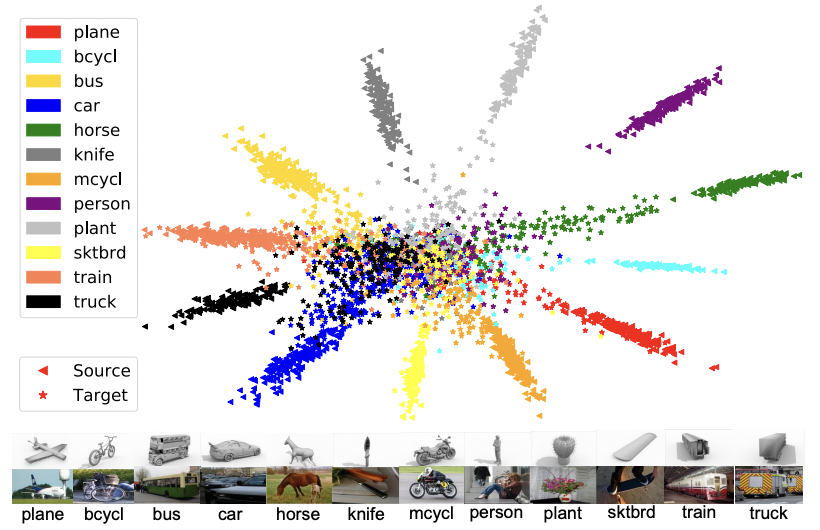
\includegraphics[width=0.7\textwidth]{chapter2/afn-visda-source-only.png}

    \caption{Visualizaci\'on de las características aprendidas para el origen y destino utilizando un modelo entrenado utilizando muestras del origen. Imagen tomada de \cite{xu2019larger}.}
    \label{fig:afn-source-only}
\end{figure}

Esto sugiere que las normas excesivamente pequeñas de las muestras de destino con respecto a las de origen explican el
deterioro en la clasificación. No obstante, pueden plantearse dos hipótesis:

\begin{itemize}
    \item Normas de las características desalineadas: el desplazamiento entre los dominios de origen y destino se explica en la
          desalineación de los valores esperados de las normas de sus características. La coincidencia de las normas de ambos
          dominios a un escalar arbitrariamente elegido supondrá una mejora en la transferencias.
    \item Norma de las caracteristicas más pequeña: el desplazamiento entre los dominios se explica debido a las características
          menos informativas con normas más pequeñas del dominio de destino. Adaptar las características de destino a regiones
          alejadas de las normas pequeñas supondrá una mejora en la transferencia.
\end{itemize}

\cite{xu2019larger} propone un método llamado {\it Adaptive Feature Norm AFN} que consiste en normalizar las normas de las características aprendidas por la red $\mathcal{G}$  mediante $n$ bloques $\mathcal{N}$ (compuestos por FC-BN-ReLU-Dropout) y mediante $\mathcal{L}_{AFN}$.

\begin{figure}[H]
    \centering

    \tikzset{every picture/.style={line width=0.75pt}} %set default line width to 0.75pt        

    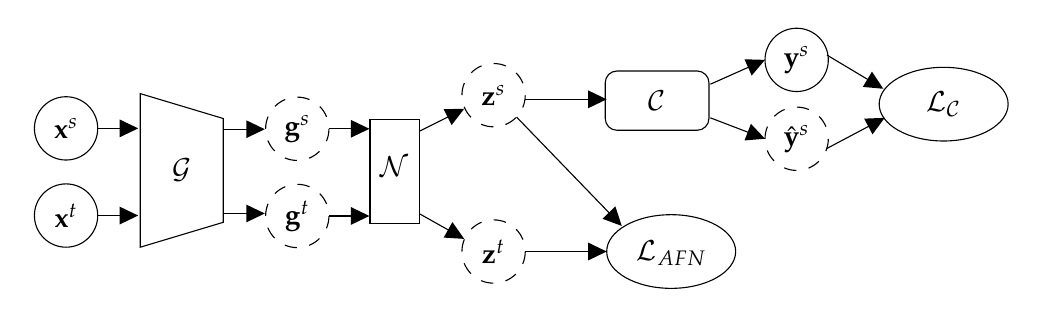
\begin{tikzpicture}[x=0.75pt,y=0.75pt,yscale=-1,xscale=1]
        %uncomment if require: \path (0,409); %set diagram left start at 0, and has height of 409

        %Shape: Circle [id:dp36883064074545446] 
        \draw   (59,84.75) .. controls (59,76.33) and (65.83,69.5) .. (74.25,69.5) .. controls (82.67,69.5) and (89.5,76.33) .. (89.5,84.75) .. controls (89.5,93.17) and (82.67,100) .. (74.25,100) .. controls (65.83,100) and (59,93.17) .. (59,84.75) -- cycle ;

        %Shape: Circle [id:dp7170555789489086] 
        \draw   (59,126.75) .. controls (59,118.33) and (65.83,111.5) .. (74.25,111.5) .. controls (82.67,111.5) and (89.5,118.33) .. (89.5,126.75) .. controls (89.5,135.17) and (82.67,142) .. (74.25,142) .. controls (65.83,142) and (59,135.17) .. (59,126.75) -- cycle ;

        %Shape: Trapezoid [id:dp6591706550778527] 
        \draw   (110,68) -- (150,80) -- (150,130) -- (110,142) -- cycle ;

        %Straight Lines [id:da8866180371172607] 
        \draw    (89.5,84.75) -- (106,84.75) ;
        \draw [shift={(109,84.75)}, rotate = 180] [fill={rgb, 255:red, 0; green, 0; blue, 0 }  ][line width=0.08]  [draw opacity=0] (8.93,-4.29) -- (0,0) -- (8.93,4.29) -- cycle    ;
        %Shape: Circle [id:dp7226735192986846] 
        \draw  [dash pattern={on 4.5pt off 4.5pt}] (264.98,68.75) .. controls (264.98,60.33) and (271.81,53.5) .. (280.23,53.5) .. controls (288.66,53.5) and (295.48,60.33) .. (295.48,68.75) .. controls (295.48,77.17) and (288.66,84) .. (280.23,84) .. controls (271.81,84) and (264.98,77.17) .. (264.98,68.75) -- cycle ;
        %Shape: Circle [id:dp11338914726883309] 
        \draw  [dash pattern={on 4.5pt off 4.5pt}] (264.98,144.08) .. controls (264.98,135.66) and (271.81,128.83) .. (280.23,128.83) .. controls (288.66,128.83) and (295.48,135.66) .. (295.48,144.08) .. controls (295.48,152.51) and (288.66,159.33) .. (280.23,159.33) .. controls (271.81,159.33) and (264.98,152.51) .. (264.98,144.08) -- cycle ;
        %Straight Lines [id:da7817124779055846] 
        \draw    (89.5,126.75) -- (106,126.75) ;
        \draw [shift={(109,126.75)}, rotate = 180] [fill={rgb, 255:red, 0; green, 0; blue, 0 }  ][line width=0.08]  [draw opacity=0] (8.93,-4.29) -- (0,0) -- (8.93,4.29) -- cycle    ;
        %Straight Lines [id:da7526972599979318] 
        \draw    (244.73,86) -- (263.38,76.67) ;
        \draw [shift={(266.07,75.33)}, rotate = 153.43] [fill={rgb, 255:red, 0; green, 0; blue, 0 }  ][line width=0.08]  [draw opacity=0] (8.93,-4.29) -- (0,0) -- (8.93,4.29) -- cycle    ;
        %Straight Lines [id:da13505401193908728] 
        \draw    (244.73,126) -- (263.45,136.53) ;
        \draw [shift={(266.07,138)}, rotate = 209.36] [fill={rgb, 255:red, 0; green, 0; blue, 0 }  ][line width=0.08]  [draw opacity=0] (8.93,-4.29) -- (0,0) -- (8.93,4.29) -- cycle    ;
        %Straight Lines [id:da4909359959704669] 
        \draw    (295.48,70.75) -- (331.73,70.75) ;
        \draw [shift={(334.73,70.75)}, rotate = 180] [fill={rgb, 255:red, 0; green, 0; blue, 0 }  ][line width=0.08]  [draw opacity=0] (8.93,-4.29) -- (0,0) -- (8.93,4.29) -- cycle    ;
        %Straight Lines [id:da25373400738229757] 
        \draw    (295.48,144.08) -- (331.73,144.08) ;
        \draw [shift={(334.73,144.08)}, rotate = 180] [fill={rgb, 255:red, 0; green, 0; blue, 0 }  ][line width=0.08]  [draw opacity=0] (8.93,-4.29) -- (0,0) -- (8.93,4.29) -- cycle    ;
        %Shape: Rectangle [id:dp03201668448552586] 
        \draw   (220.67,80.6) -- (244.33,80.6) -- (244.33,130.4) -- (220.67,130.4) -- cycle ;

        %Shape: Circle [id:dp0590517882755186] 
        \draw  [dash pattern={on 4.5pt off 4.5pt}] (170.4,84.95) .. controls (170.4,76.53) and (177.23,69.7) .. (185.65,69.7) .. controls (194.07,69.7) and (200.9,76.53) .. (200.9,84.95) .. controls (200.9,93.37) and (194.07,100.2) .. (185.65,100.2) .. controls (177.23,100.2) and (170.4,93.37) .. (170.4,84.95) -- cycle ;
        %Shape: Circle [id:dp9792876246953977] 
        \draw  [dash pattern={on 4.5pt off 4.5pt}] (170.4,126.95) .. controls (170.4,118.53) and (177.23,111.7) .. (185.65,111.7) .. controls (194.07,111.7) and (200.9,118.53) .. (200.9,126.95) .. controls (200.9,135.37) and (194.07,142.2) .. (185.65,142.2) .. controls (177.23,142.2) and (170.4,135.37) .. (170.4,126.95) -- cycle ;
        %Straight Lines [id:da9352682997505948] 
        \draw    (200.9,84.95) -- (217.4,84.95) ;
        \draw [shift={(220.4,84.95)}, rotate = 180] [fill={rgb, 255:red, 0; green, 0; blue, 0 }  ][line width=0.08]  [draw opacity=0] (8.93,-4.29) -- (0,0) -- (8.93,4.29) -- cycle    ;
        %Straight Lines [id:da9288909607910223] 
        \draw    (200.9,126.95) -- (217.4,126.95) ;
        \draw [shift={(220.4,126.95)}, rotate = 180] [fill={rgb, 255:red, 0; green, 0; blue, 0 }  ][line width=0.08]  [draw opacity=0] (8.93,-4.29) -- (0,0) -- (8.93,4.29) -- cycle    ;
        %Straight Lines [id:da42477525756570467] 
        \draw    (150.5,85.15) -- (167,85.15) ;
        \draw [shift={(170,85.15)}, rotate = 180] [fill={rgb, 255:red, 0; green, 0; blue, 0 }  ][line width=0.08]  [draw opacity=0] (8.93,-4.29) -- (0,0) -- (8.93,4.29) -- cycle    ;
        %Straight Lines [id:da19510792007996902] 
        \draw    (150.5,125.75) -- (167,125.75) ;
        \draw [shift={(170,125.75)}, rotate = 180] [fill={rgb, 255:red, 0; green, 0; blue, 0 }  ][line width=0.08]  [draw opacity=0] (8.93,-4.29) -- (0,0) -- (8.93,4.29) -- cycle    ;
        %Rounded Rect [id:dp8233373593250533] 
        \draw   (334,62.81) .. controls (334,59.65) and (336.56,57.1) .. (339.71,57.1) -- (378.29,57.1) .. controls (381.44,57.1) and (384,59.65) .. (384,62.81) -- (384,79.95) .. controls (384,83.11) and (381.44,85.67) .. (378.29,85.67) -- (339.71,85.67) .. controls (336.56,85.67) and (334,83.11) .. (334,79.95) -- cycle ;

        %Shape: Circle [id:dp361141070335256] 
        \draw   (411,51.75) .. controls (411,43.33) and (417.83,36.5) .. (426.25,36.5) .. controls (434.67,36.5) and (441.5,43.33) .. (441.5,51.75) .. controls (441.5,60.17) and (434.67,67) .. (426.25,67) .. controls (417.83,67) and (411,60.17) .. (411,51.75) -- cycle ;
        %Shape: Circle [id:dp994981759860698] 
        \draw  [dash pattern={on 4.5pt off 4.5pt}] (411,89.75) .. controls (411,81.33) and (417.83,74.5) .. (426.25,74.5) .. controls (434.67,74.5) and (441.5,81.33) .. (441.5,89.75) .. controls (441.5,98.17) and (434.67,105) .. (426.25,105) .. controls (417.83,105) and (411,98.17) .. (411,89.75) -- cycle ;
        %Shape: Ellipse [id:dp4863694749188221] 
        \draw   (466,73.08) .. controls (466,63.28) and (479.91,55.33) .. (497.06,55.33) .. controls (514.22,55.33) and (528.13,63.28) .. (528.13,73.08) .. controls (528.13,82.89) and (514.22,90.83) .. (497.06,90.83) .. controls (479.91,90.83) and (466,82.89) .. (466,73.08) -- cycle ;
        %Straight Lines [id:da7034112467211542] 
        \draw    (384.67,63.48) -- (408.26,52.97) ;
        \draw [shift={(411,51.75)}, rotate = 156] [fill={rgb, 255:red, 0; green, 0; blue, 0 }  ][line width=0.08]  [draw opacity=0] (8.93,-4.29) -- (0,0) -- (8.93,4.29) -- cycle    ;
        %Straight Lines [id:da28235679904283506] 
        \draw    (384.67,79.67) -- (408.2,88.68) ;
        \draw [shift={(411,89.75)}, rotate = 200.95] [fill={rgb, 255:red, 0; green, 0; blue, 0 }  ][line width=0.08]  [draw opacity=0] (8.93,-4.29) -- (0,0) -- (8.93,4.29) -- cycle    ;
        %Straight Lines [id:da3443605473479898] 
        \draw    (440.83,49.42) -- (465.43,64.13) ;
        \draw [shift={(468,65.67)}, rotate = 210.89] [fill={rgb, 255:red, 0; green, 0; blue, 0 }  ][line width=0.08]  [draw opacity=0] (8.93,-4.29) -- (0,0) -- (8.93,4.29) -- cycle    ;
        %Straight Lines [id:da6547044180228383] 
        \draw    (440.83,94.42) -- (466.02,81.07) ;
        \draw [shift={(468.67,79.67)}, rotate = 152.08] [fill={rgb, 255:red, 0; green, 0; blue, 0 }  ][line width=0.08]  [draw opacity=0] (8.93,-4.29) -- (0,0) -- (8.93,4.29) -- cycle    ;
        %Straight Lines [id:da7710823975987622] 
        \draw    (291.33,79.33) -- (339.91,129.59) ;
        \draw [shift={(342,131.75)}, rotate = 225.97] [fill={rgb, 255:red, 0; green, 0; blue, 0 }  ][line width=0.08]  [draw opacity=0] (8.93,-4.29) -- (0,0) -- (8.93,4.29) -- cycle    ;
        %Shape: Ellipse [id:dp8075338571919093] 
        \draw   (334.73,144.08) .. controls (334.73,134.28) and (348.64,126.33) .. (365.8,126.33) .. controls (382.95,126.33) and (396.86,134.28) .. (396.86,144.08) .. controls (396.86,153.89) and (382.95,161.83) .. (365.8,161.83) .. controls (348.64,161.83) and (334.73,153.89) .. (334.73,144.08) -- cycle ;

        % Text Node
        \draw (130,105) node   [align=left] {\begin{minipage}[lt]{22.78pt}\setlength\topsep{0pt}
                \begin{center}
                    $\mathcal{G}$
                \end{center}

            \end{minipage}};
        % Text Node
        \draw (74.25,126.75) node   [align=left] {\begin{minipage}[lt]{21.08pt}\setlength\topsep{0pt}
                \begin{center}
                    $\mathbf{x}^t$
                \end{center}

            \end{minipage}};
        % Text Node
        \draw (74.25,84.75) node   [align=left] {\begin{minipage}[lt]{21.08pt}\setlength\topsep{0pt}
                \begin{center}
                    $\mathbf{x}^s$
                \end{center}

            \end{minipage}};
        % Text Node
        \draw (221,97.4) node [anchor=north west][inner sep=0.75pt]   [align=left] {\begin{minipage}[lt]{15pt}\setlength\topsep{0pt}
                \begin{center}
                    $\mathcal{N}$
                \end{center}

            \end{minipage}};
        % Text Node
        \draw (185.65,84.95) node   [align=left] {\begin{minipage}[lt]{21.08pt}\setlength\topsep{0pt}
                \begin{center}
                    $\mathbf{g}^s$
                \end{center}

            \end{minipage}};
        % Text Node
        \draw (185.65,126.95) node   [align=left] {\begin{minipage}[lt]{21.08pt}\setlength\topsep{0pt}
                \begin{center}
                    $\mathbf{g}^t$
                \end{center}

            \end{minipage}};
        % Text Node
        \draw (426.25,51.75) node   [align=left] {\begin{minipage}[lt]{21.08pt}\setlength\topsep{0pt}
                \begin{center}
                    $\mathbf{y}^s$
                \end{center}

            \end{minipage}};
        % Text Node
        \draw (426.25,89.75) node   [align=left] {\begin{minipage}[lt]{21.08pt}\setlength\topsep{0pt}
                \begin{center}
                    $\hat{\mathbf{y}}^s$
                \end{center}

            \end{minipage}};
        % Text Node
        \draw (497.06,73.08) node   [align=left] {\begin{minipage}[lt]{32.64pt}\setlength\topsep{0pt}
                \begin{center}
                    $\mathcal{L}_{\mathcal{C}}$
                \end{center}

            \end{minipage}};
        % Text Node
        \draw (359,71.56) node   [align=left] {\begin{minipage}[lt]{26.23pt}\setlength\topsep{0pt}
                \begin{center}
                    $\mathcal{C}$
                \end{center}

            \end{minipage}};
        % Text Node
        \draw (366,145) node   [align=left] {\begin{minipage}[lt]{35pt}\setlength\topsep{0pt}
                \begin{center}
                    $\mathcal{L}_{AFN}$
                \end{center}

            \end{minipage}};
        % Text Node
        \draw (280.23,144.08) node   [align=left] {\begin{minipage}[lt]{21.08pt}\setlength\topsep{0pt}
                \begin{center}
                    $\mathbf{z}^t$
                \end{center}

            \end{minipage}};
        % Text Node
        \draw (280.23,68.75) node   [align=left] {\begin{minipage}[lt]{21.08pt}\setlength\topsep{0pt}
                \begin{center}
                    $\mathbf{z}^s$
                \end{center}

            \end{minipage}};

    \end{tikzpicture}
    \caption{Esquema de {\it AFN}. Los supra indices $s$ y $t$ indican si los datos son del origen o destino respectivamente.
    Los c\'irculos con l\'ineas rayadas son salidas de los modelos mientras que los c\'irculos de l\'ineas s\'olidas son datos conocidos. El modelo {\it backbone} $\mathcal{G}$ produce características $\mathbf{x}$ que luego son aplicadas por bloques $\mathcal{N}$ (FC-BN-ReLU-Dropout) produciendo características normalizadas $\mathbf{d}$. La red clasificadora $\mathcal{C}$ toma las características $\mathbf{d}^s$ y se computa $\mathcal{L}_{\mathcal{C}}$. $\mathcal{L}_{AFN}$ se calcula utilizando $\mathbf{d}$.}
    \label{fig:afn-esquema}
\end{figure}

En su variante iterativa, $\mathcal{L}_{AFN}$ se define como:

\begin{align}
    \min_{\mathcal{G}} \mathcal{L}_{AFN}(\mathbf{x}^s, \mathbf{x}^t) = & \mathbb{E}_{\mathbf{x}^s \sim \mathcal{\hat{S}}} \mathbb{E}[(\| \mathcal{G}(\mathcal{N}(\mathbf{x}^s)) \| - \Delta_r)^2] \nonumber \\
                                                                       & + \mathbb{E}_{\mathbf{x}^t \sim \mathcal{\hat{T}}} \mathbb{E}[(\| \mathcal{G}(\mathcal{N}(\mathbf{x}^t)) \| - \Delta_r)^2]
    \label{eq:afn-loss}
\end{align}

Donde $\Delta_r$ corresponde al escalar que controla la amplitud de la norma. Los autores afirman que puede agregarse
un término a la ecuación \ref{eq:afn-loss} respecto a la entropía $\mathcal{H}$ de la función {\it softmax} $\sigma$
para facilitar la discriminabilidad mediante un factor $\beta$:

\begin{align}
    \min_{\mathcal{G}} \mathcal{L}_{AFN}(\mathbf{x}^s, \mathbf{x}^t) = & \mathbb{E}_{\mathbf{x}^s \sim \mathcal{\hat{S}}} \mathbb{E}[(\| \mathcal{G}(\mathcal{N}(\mathbf{x}^s)) \| - \Delta_r)^2] \nonumber   \\
                                                                       & + \mathbb{E}_{\mathbf{x}^t \sim \mathcal{\hat{T}}} \mathbb{E}[(\| \mathcal{G}(\mathcal{N}(\mathbf{x}^t)) \| - \Delta_r)^2] \nonumber \\
                                                                       & + \beta \mathcal{H}(\sigma(\mathcal{G}(\mathcal{N}(\mathbf{x}^s)) ))
    \label{eq:afn-loss-entropy}
\end{align}

Por lo tanto, el objetivo de optimización viene dado por la ecuaci\'on \ref{eq:afn-objetivo}, donde $\lambda$ es el
trade-off entre la clasificaci\'on y normalizacion de normas.

\begin{align}
    \min_{\mathcal{G}, \mathcal{C}} \mathcal{L}_{\mathcal{C}}(\mathbf{x}^s, \mathbf{x}^t) + \lambda \mathcal{L}_{\mathcal{AFN}}(\mathbf{x}^s, \mathbf{x}^t)
    \label{eq:afn-objetivo}
\end{align}
\chapter{Metodolog\'ia}

\label{Chapter3}

En este cap\'itulo se detallar\'an los procesos abordados para la extracci\'on y clasificaci\'on de los d\'igitos
escritos en los telegramas de las elecciones. Primero se describir\'a el proceso de obtenci\'on, limpieza y
transformaci\'on de los datos a fin de obtener un dataset con el cual entrenar. Luego, se describir\'an los procesos a
ser llevados a cabo para el dise\~{n}o experimental de los modelos.

\section{Descripci\'on de los datos}

Los telegramas fueron descargados desde la \href{https://op.elecciones.gob.ar/telegramas/generales2021/}{p\'agina
    oficial del estado argentino}. Presentan un formato est\'andar en forma de grilla donde en cada rengl\'on se encuentra
el partido pol\'itico y los votos obtenidos para diputados y senadores. En la p\'agina tambi\'en se puede descargar un
CSV donde se encuentra el {\it id} de cada telegrama y los valores digitalizados oficialmente.

\section{Extracci\'on de d\'igitos de los telegramas}

Los telegramas de las elecciones de Santa Fe presentan un formato tabular, donde cada fila representa un partido
pol\'itico y los votos obtenidos abiertos por senadores y diputados. Se debieron ejecutar m\'ultiples pasos de
extracci\'on, transformaci\'on y carga (ETL por sus siglas) de los mismos antes de poder armar un dataset con el cual
entrenar los modelos. Se utiliz\'o la librer\'ia OpenCV \parencite{opencv_library} para manipular las im\'agenes y poder llevar a cabo el proceso de ETL.

\subsection{Enderezado}
Como los telegramas son escaneados a mano, el primer paso consiste en enderezarlos. Este proceso puede realizarse
buscando el rect\'angulo de mayor \'area, calculando el \'angulo de rotaci\'on y rotando la imagen completa con la
funci\'on \verb|getRotationMatrix2D| de OpenCV.

\begin{figure}[H]
    \centering

    \tikzset{every picture/.style={line width=0.75pt}}

    \begin{tikzpicture}[x=0.75pt,y=0.75pt,yscale=-1,xscale=1]

        \draw (370,140) node  {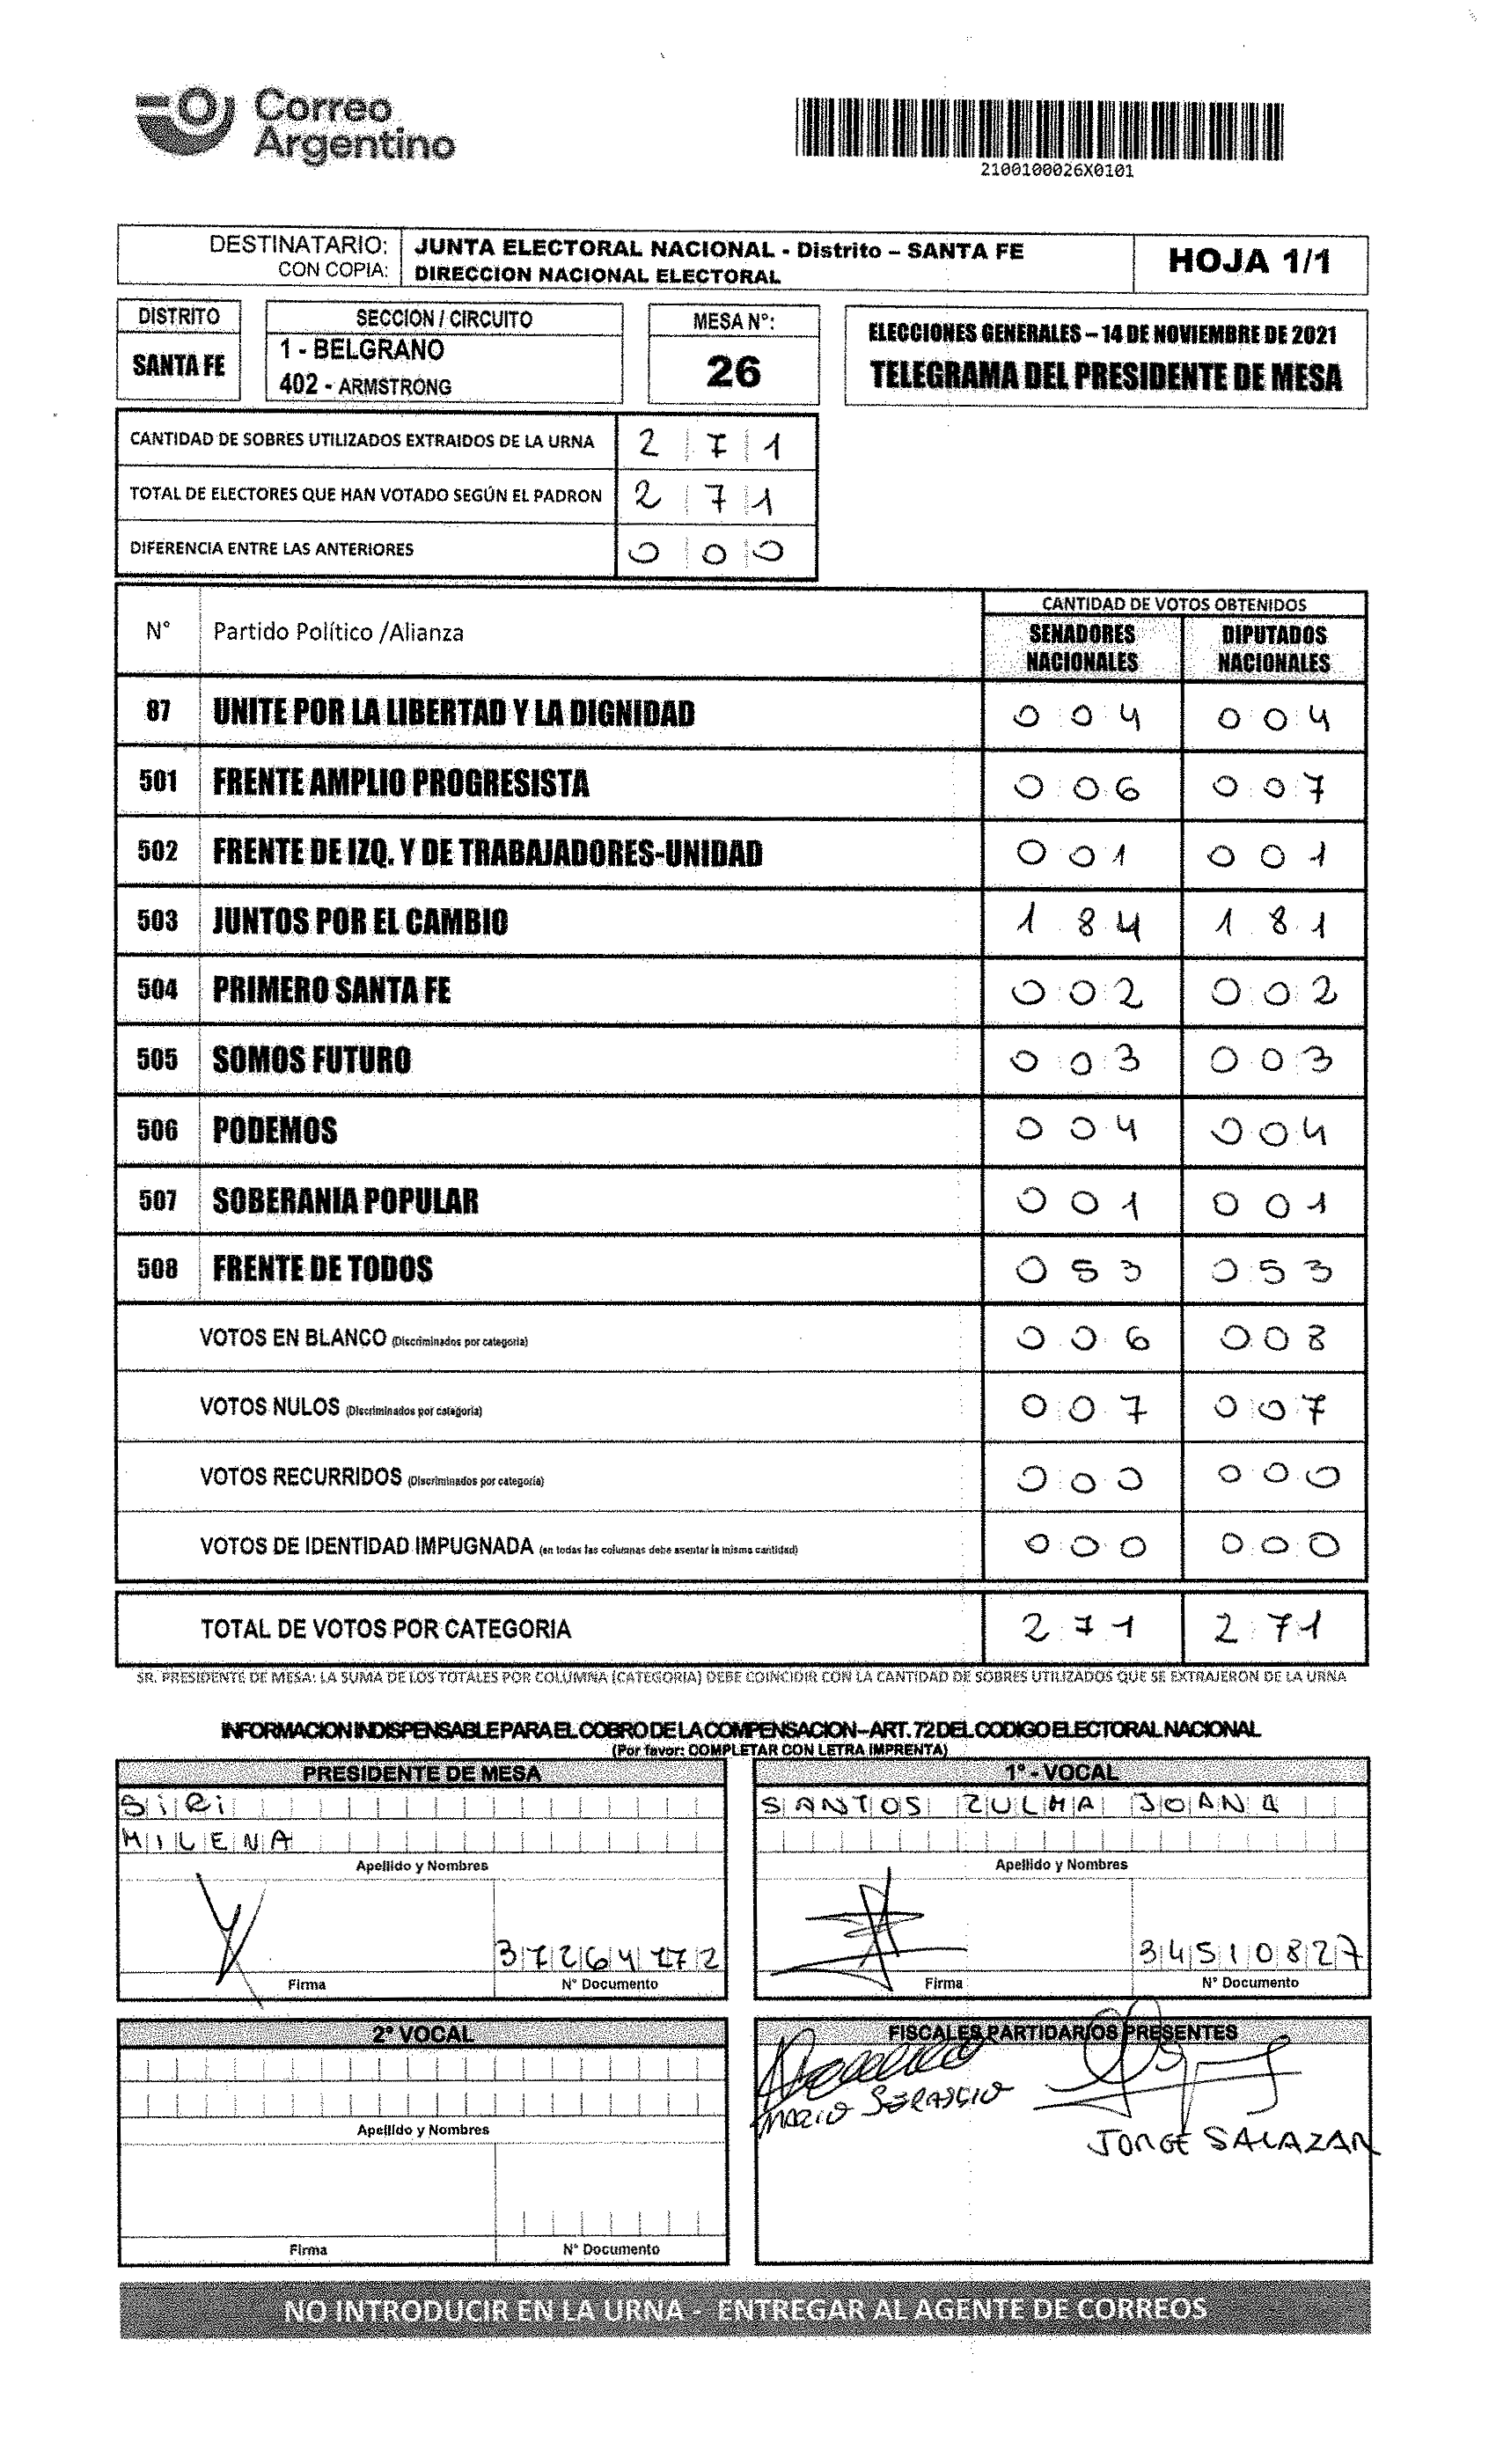
\includegraphics[width=135pt,height=210pt]{chapter3/etl-1-rotacion.png}};
        \draw (90,140) node  {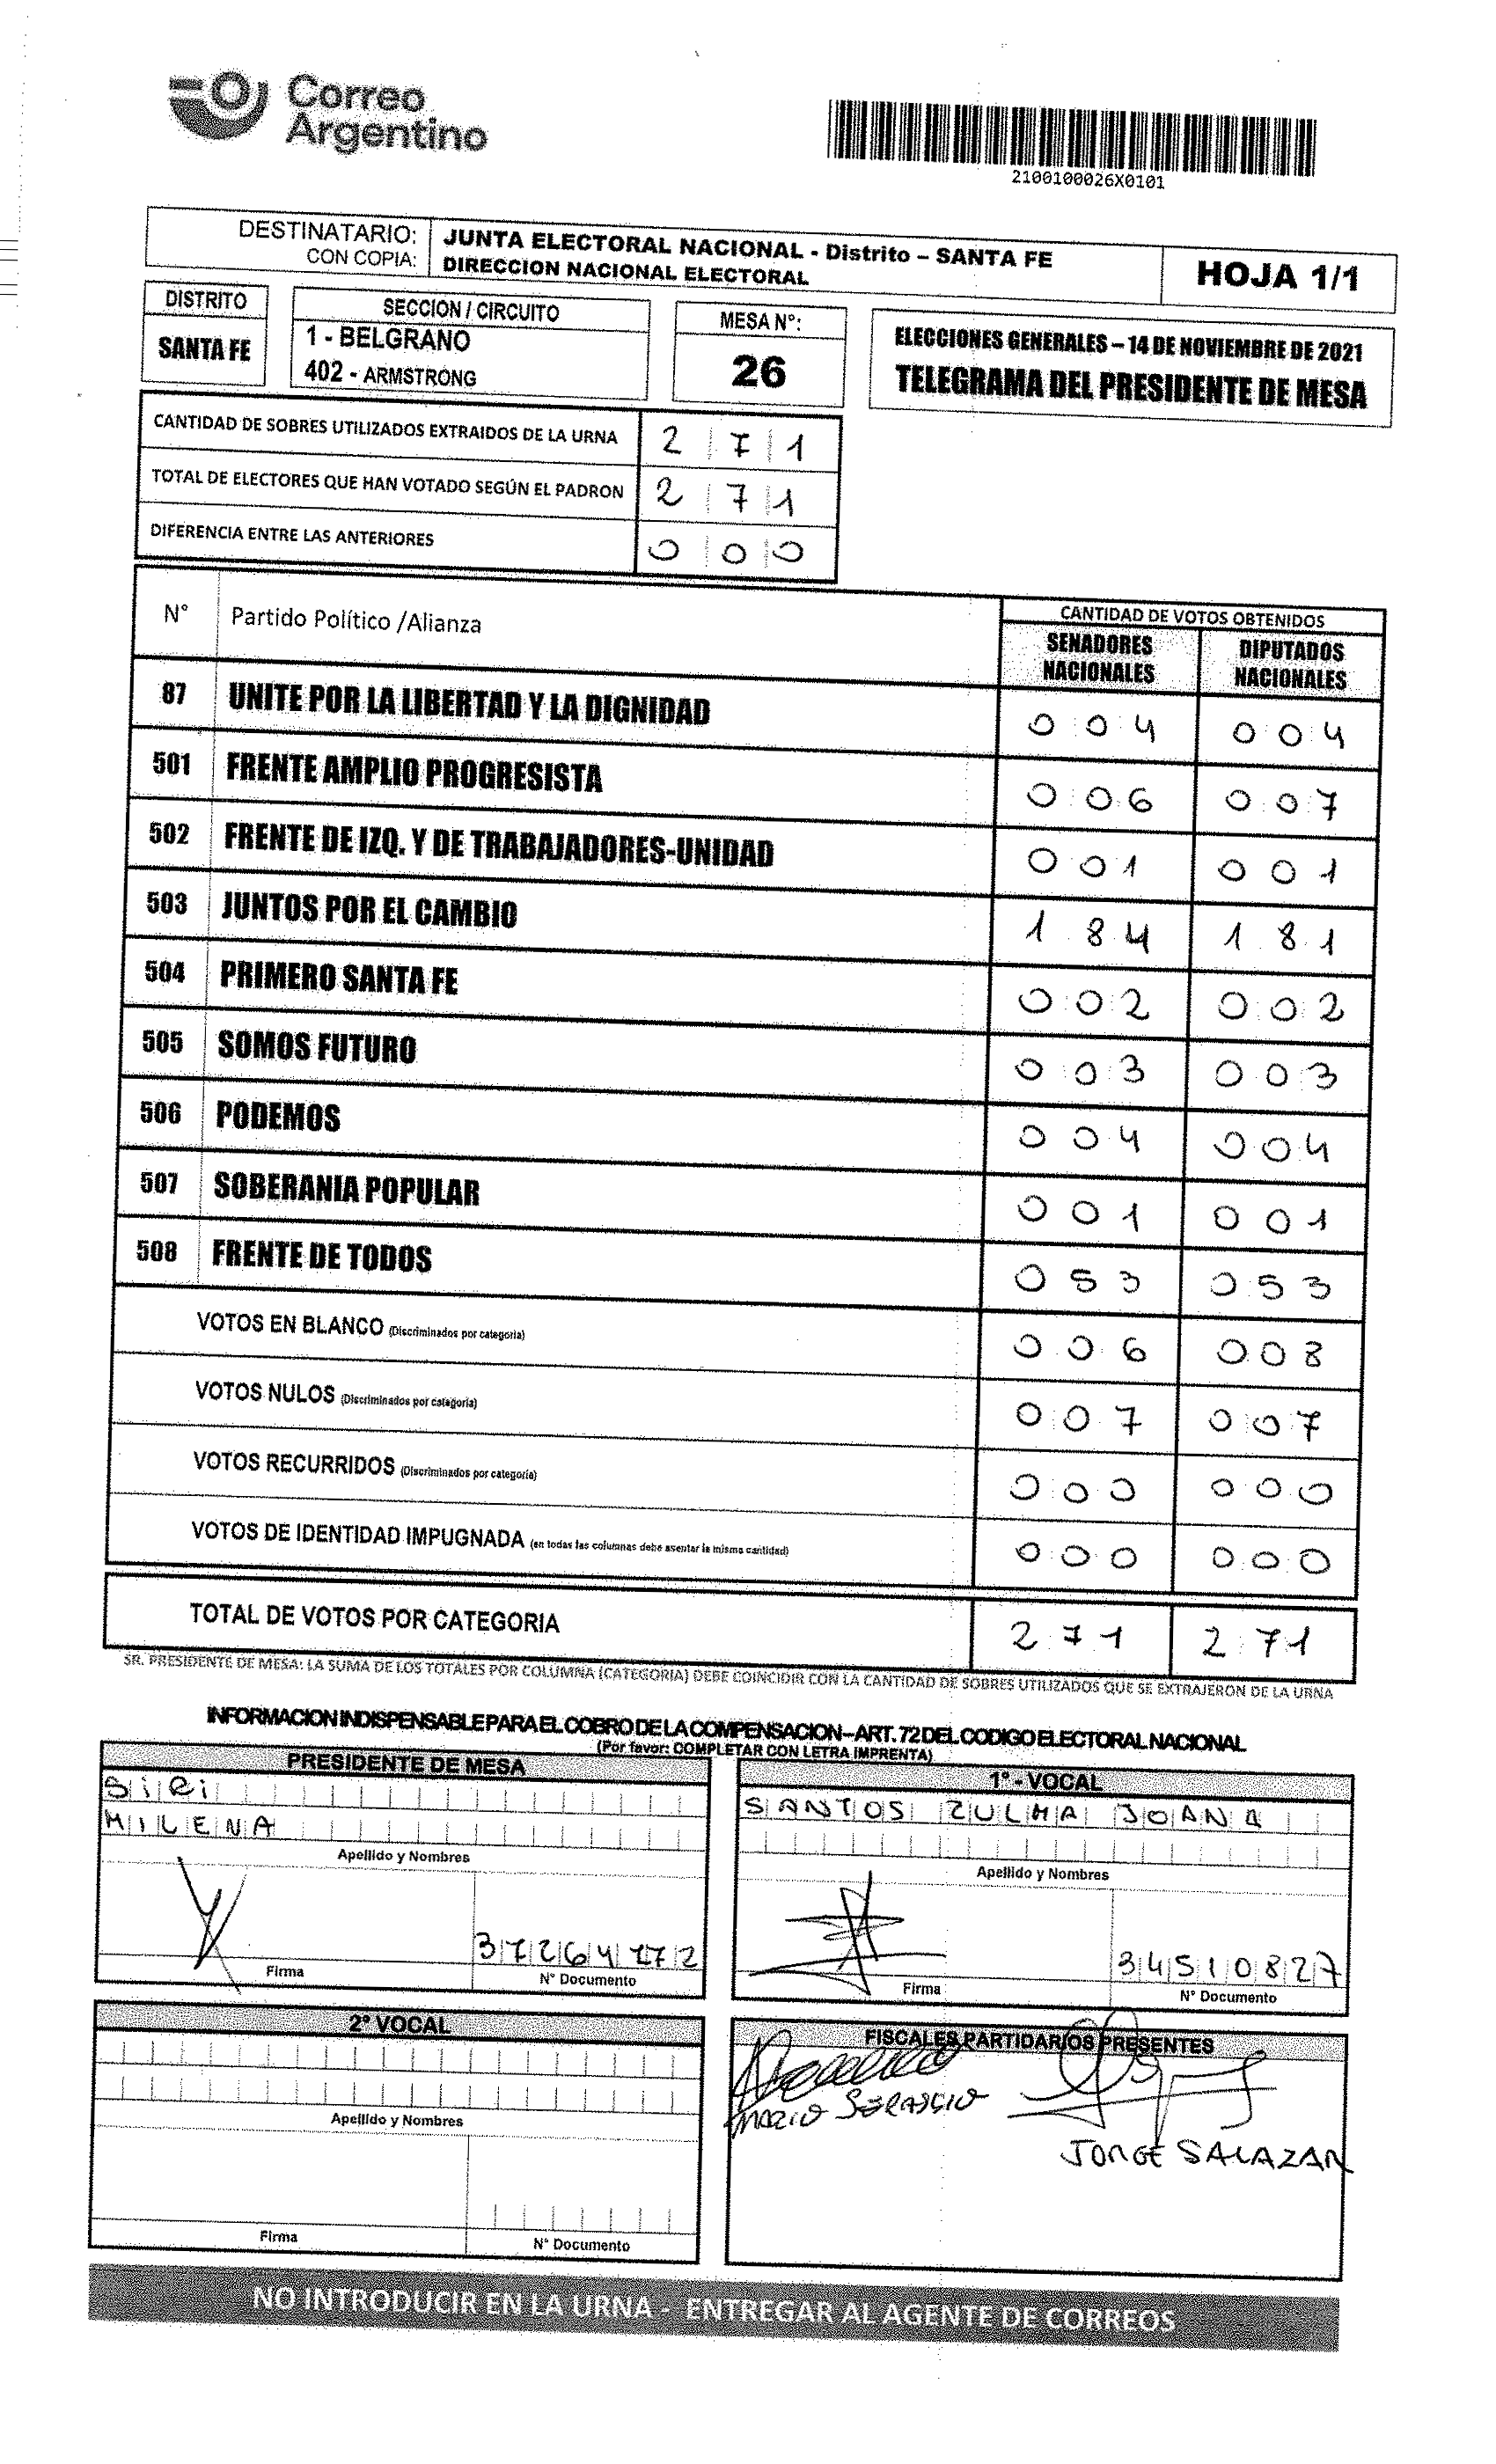
\includegraphics[width=135pt,height=210pt]{chapter3/etl-1-telegrama.png}};
        \draw    (190.8,110.6) -- (267.4,110.6) ;
        \draw [shift={(269.4,110.6)}, rotate = 180] [color={rgb, 255:red, 0; green, 0; blue, 0 }  ][line width=0.75]    (10.93,-3.29) .. controls (6.95,-1.4) and (3.31,-0.3) .. (0,0) .. controls (3.31,0.3) and (6.95,1.4) .. (10.93,3.29)   ;
        \draw (190,87.18) node [anchor=north west][inner sep=0.75pt]   [align=left] {Enderezar};

    \end{tikzpicture}

    \caption{Enderezamiento de un telegrama utilizando OpenCV.}
    \label{fig:etl-1-rotacion}
\end{figure}

\subsection{Extracci\'on de la grilla de votos}
El siguiente paso consiste en poder seleccionar la grilla de los votos y poder extraerla para seguir trabajando en
ella. Esto puede realizarse utilizando la funcion \verb|getContours| de OpenCV y qued\'andose con el contorno de mayor
\'area.

\begin{figure}[H]
    \centering
    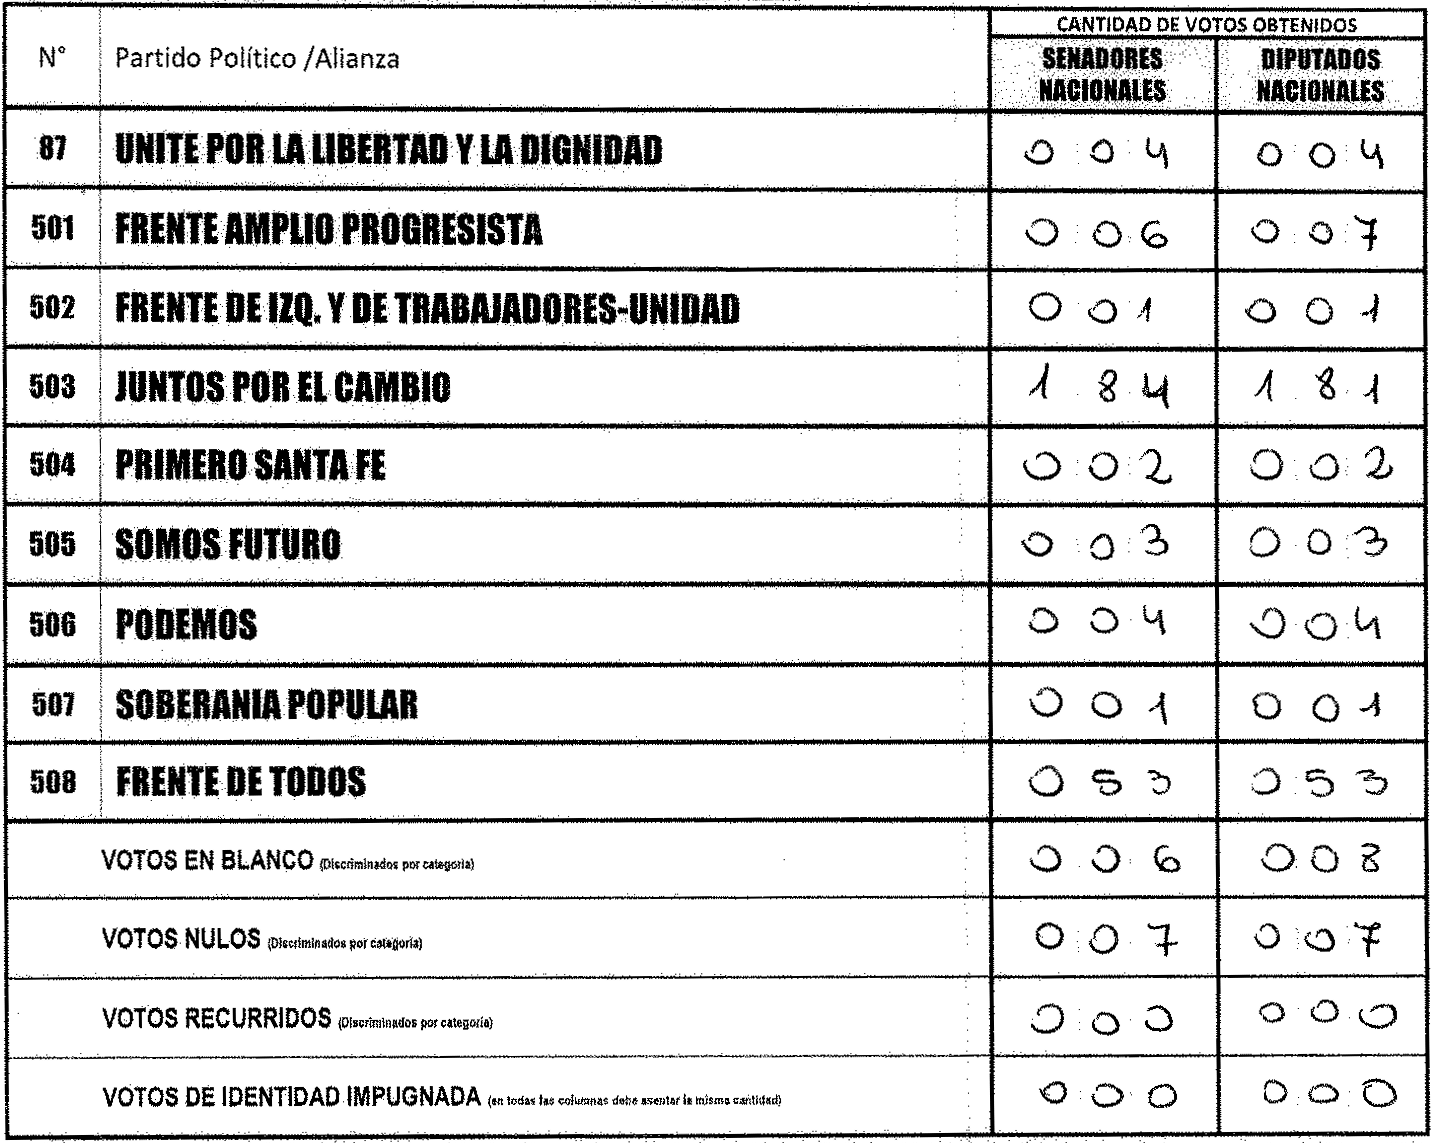
\includegraphics[width=0.4\textwidth, height=0.3\textwidth]{chapter3/etl-2-grilla.png}
    \caption{Grilla de votos extra\'ida buscando el contorno de mayor \'area.}
    \label{fig:etl-2-grilla}
\end{figure}

\subsection{Detecci\'on de l\'ineas de la grilla de votos}
Teniendo la grilla de votos separada del telegrama, se procede a detectar las l\'ineas para poder extraer cada registro
de la misma. Si bien OpenCV posee funciones para la detecci\'on de l\'ineas, se opt\'o por utilizar un enfoque
simplificado. El mismo es similar al utilizado en \parencite{lamagna2016lectura}. Debido a que la grilla se encuentra enderezada, se puede utilizar proyecciones de los
colores sobre los ejes $x$ e $y$ para detectarlas. Al sumar todos los colores por eje, se pueden encontrar los picos
donde se encuentran las lineas horizontales y verticales. Posteriormente, se selecciona un umbral de corte por cada
eje, siendo el promedio menos dos desv\'ios est\'andar. La figura \ref{fig:etl-3-proyecciones} muestra las proyecciones
obtenidas con los umbrales por cada eje.

\begin{figure}
    \centering

    \tikzset{every picture/.style={line width=0.75pt}}

    \begin{tikzpicture}[x=0.75pt,y=0.75pt,yscale=-1,xscale=1]
        \draw (142.77,162.65) node  {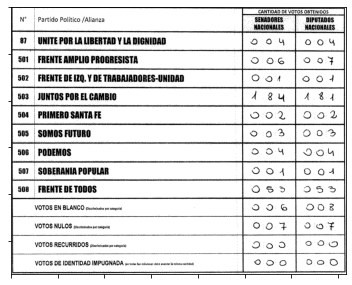
\includegraphics[width=214.16pt,height=173.4pt]{chapter3/etl-3-grilla.png}};
        \draw (303.6,159.11) node [rotate=-90] {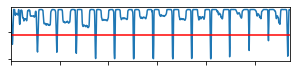
\includegraphics[width=172pt,height=46.15pt]{chapter3/etl-3-grilla-proyeccion-y.png}};
        \draw (142.5,30.77) node  {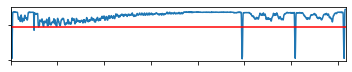
\includegraphics[width=213.75pt,height=46.15pt]{chapter3/etl-3-grilla-proyeccion-x.png}};
    \end{tikzpicture}

    \caption{Proyecciones de los ejes de la grilla. En rojo se marca el umbral de corte.}
    \label{fig:etl-3-proyecciones}
\end{figure}

Sin embargo, aunque se seleccione aquellos pixeles que se encuentren por debajo del umbral, por cada pico existe mas de
un pixel. Siguiendo con el ejemplo, en el eje $x$ se obtienen los siguientes pixeles que se encuentran en los "picos":

\begin{verbatim}
    array([    3,    4,    5,    6,    7,  100,  119,  120,  988, 
             989,  990,  991,  992, 1215, 1216, 1217, 1218, 1219, 
            1423, 1424, 1425, 1426, 1427])
\end{verbatim}

Con la estrategia del umbral no se obtienen las 4 l\'ineas que se desean detectar sobre el eje $x$. No obstante, se
puede aplicar un clustering jer\'arquico sobre los \'indices obtenidos y luego calcular el \'indice promedio de cada
cluster para tomarlo como \'unico representante. El proceso se repite de la misma manera sobre el eje $y$. Esta
\'ultima modificaci\'on sobre el trabajo realizado en \parencite{lamagna2016lectura} asegura tener un \'unico pixel por l\'inea.

\begin{figure}[H]
    \centering
    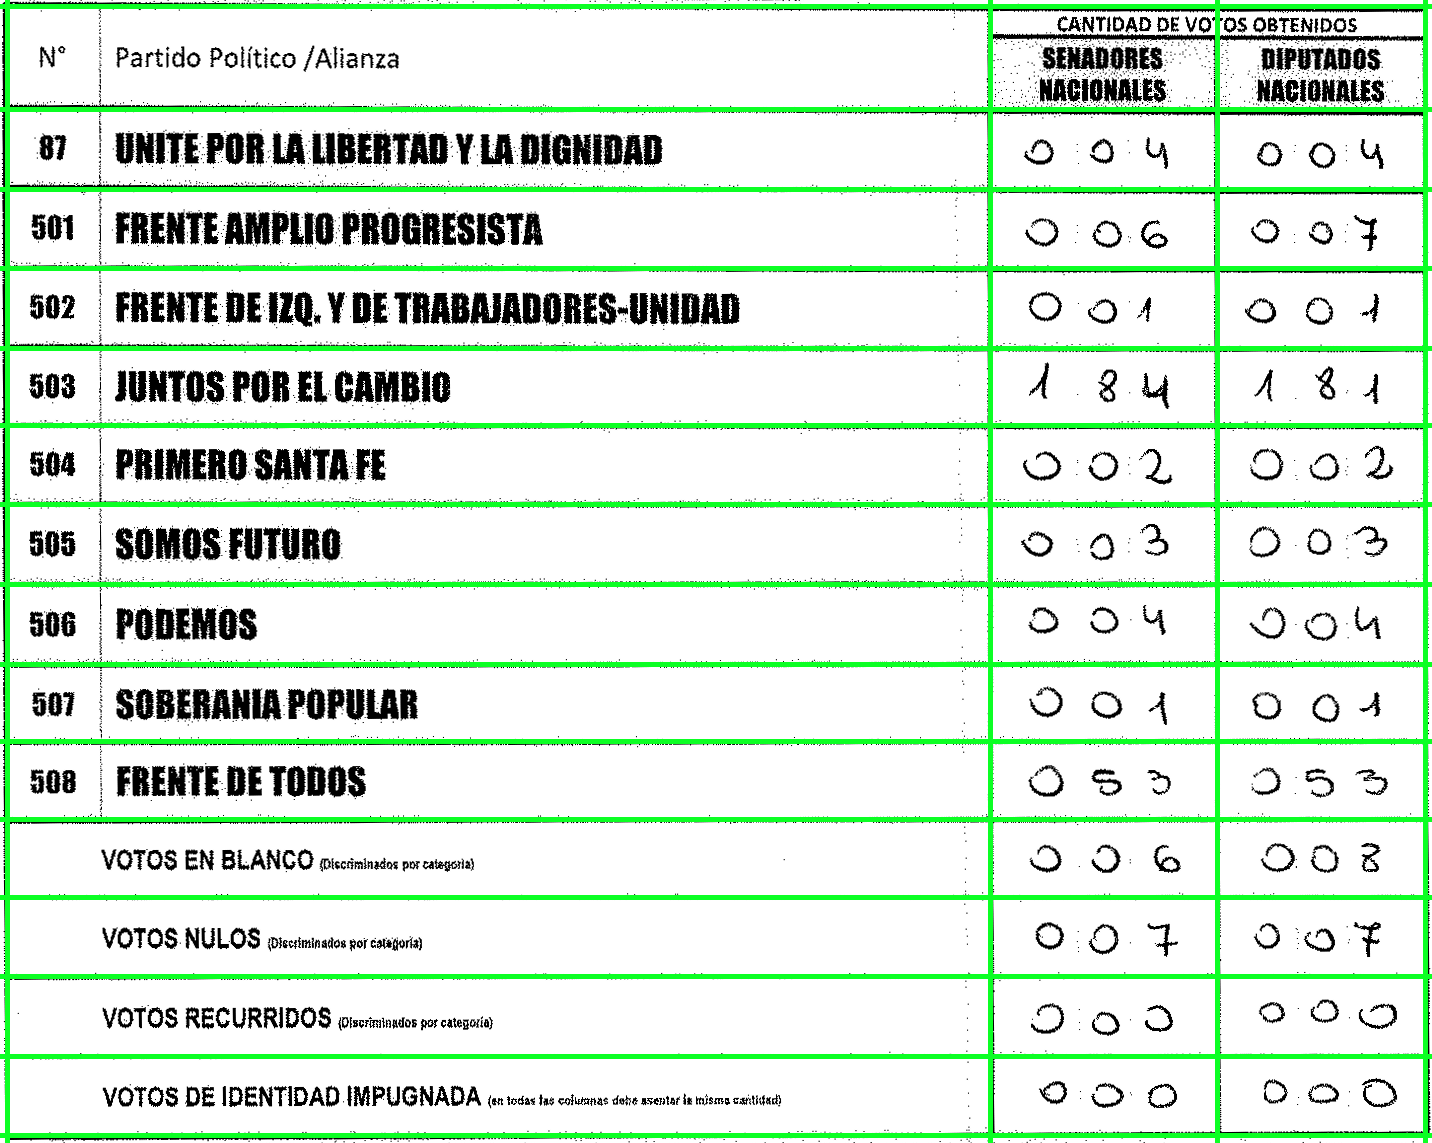
\includegraphics[width=0.4\textwidth, height=0.3\textwidth]{chapter3/etl-3-grilla-detectada.png}
    \caption{Grilla detectada (en verde) utilizando el umbral por sobre las proyecciones y su posterior agrupamiento con clustering jer\'arquico.}
    \label{fig:etl-3-grilla-detectada}
\end{figure}

\subsection{Segmentaci\'on de d\'igitos}

Una vez obtenida la grilla, se itera por cada registro obteniendo los rect\'angulos que contienen los votos, ignorando
el primer rengl\'on que contiene los t\'itulos de la grilla.

\begin{figure}[H]
    \centering
    \frame{
\includegraphics[height=15pt]{chapter3/etl-4-registro-1.png}}
    \frame{
\includegraphics[height=15pt]{chapter3/etl-4-registro-2.png}}
    \frame{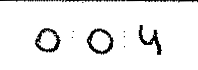
\includegraphics[height=15pt]{chapter3/etl-4-registro-3.png}}
    \caption{Primer registro extra\'ido de la grilla de votos.}
    \label{fig:etl-4-registro}
\end{figure}

Para separar cada d\'igito en una \'unica imagen, se utiliza un an\'alisis de componentes conectados
(\verb|connectedComponents| de OpenCV) y se recortan aquellos contornos que posean de \'area entre el $5\%$ y el $70\%$
de los pixeles totales de la imagen. Los valores fueron obtenidos mediante experimentaci\'on y sirven para descartar
ruido que pueda detectar el an\'alisis de componentes conectados.

\begin{figure}[H]
    \centering
    \frame{
\includegraphics[height=15pt]{chapter3/etl-4-digito-1.png}}
    \frame{
\includegraphics[height=15pt]{chapter3/etl-4-digito-2.png}}
    \frame{
\includegraphics[height=15pt]{chapter3/etl-4-digito-3.png}}
    \caption{D\'igitos detectados en el primer bloque de votos.}
    \label{fig:etl-4-digitos}
\end{figure}

Por \'ultimo, los d\'igitos se guardan de forma que sean cuadrados junto a su etiqueta tomada de la digitalizaci\'on
oficial. El dataset ser\'a denominado como {\it TDS} (dataset de telegramas) a lo largo de la presente tesis.

\section{An\'alisis del dataset}

Con la estracci\'on descripta en la secci\'on anterior, se procede a hacer un an\'alisis exploratorio de los datos en
b\'usqueda de posibles errores. La tabla \ref{tab:dataset-telegramas-segmentados} muestra algunos registros del dataset
que vincula los d\'igitos extra\'idos de los telegramas con los partidos pol\'iticos.

\begin{table}[H]
    \centering
    \begin{tabular}{ccccc}
        \toprule
        Telegrama                                                                & Partido & Tipo      & D\'igitos                                                                & Cantidad D\'igitos \\
        \midrule
        2100100026X                                                              & Unite   & Diputados & \frame{
\includegraphics[width=16px]{chapter3/eda/unite-diputados-1.png}}
        \frame{
\includegraphics[width=16px]{chapter3/eda/unite-diputados-2.png}}
        \frame{
\includegraphics[width=16px]{chapter3/eda/unite-diputados-3.png}} & 3                                                                                                                   \\
        2100100026X                                                              & Unite   & Senadores & \frame{
\includegraphics[width=16px]{chapter3/eda/unite-senadores-1.png}}
        \frame{
\includegraphics[width=16px]{chapter3/eda/unite-senadores-2.png}}
        \frame{
\includegraphics[width=16px]{chapter3/eda/unite-senadores-3.png}}
        \frame{
\includegraphics[width=16px]{chapter3/eda/unite-senadores-4.png}} & 4                                                                                                                   \\
        \bottomrule

    \end{tabular}
    \caption{Ejemplo de registros del dataset.}
    \label{tab:dataset-telegramas-segmentados}
\end{table}

El lector podr\'a darse cuenta que existen errores en el cuadro anterior. En la columna de d\'igitos donde se deber\'ia
encontrar s\'olamente n\'umeros existe uno incorrecto para senadores. Para limpiar estas extracciones incorrectas, se
calculan dos columnas las cuales contienen la proporci\'on m\'inima y m\'axima de pixeles blancos en las im\'agenes. La
figura \ref{fig:histogramas-min-max-prop-blanco} muestra los histogramas generales de estas dos variables.

\begin{figure}[H]
    \centering
    \begin{subfigure}[h]{0.48\textwidth}
        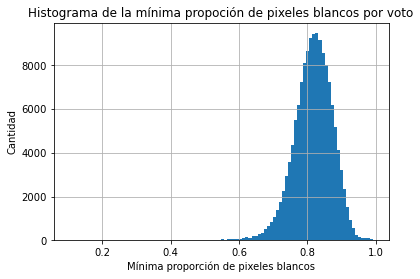
\includegraphics[width=1\textwidth]{chapter3/eda/hist-min-prop-blanco.png}
        \caption{Dominios distintos, discriminables.}
        \label{fig:histograma-min-prop-blanco}
    \end{subfigure}
    \hfill
    \begin{subfigure}[h]{0.48\textwidth}
        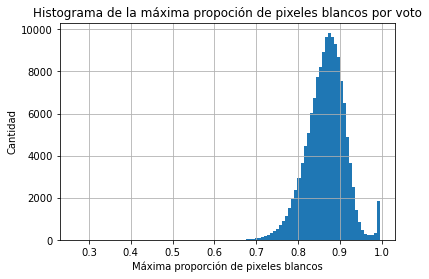
\includegraphics[width=1\textwidth]{chapter3/eda/hist-max-prop-blanco.png}
        \caption{Dominios distintos, discriminables.}
        \label{fig:histograma-max-prop-blanco}
    \end{subfigure}
    \caption{algo}
    \label{fig:histogramas-min-max-prop-blanco}
\end{figure}

\section{Dise\~{n}o experimental}

\lipsum[1]

\section{M\'etricas de evaluaci\'on}

Los modelos entrenados ser\'an evaluados con distintas m\'etricas, descriptas en las siguientes sub-secciones del
cap\'itulo. Las mismas pretenden evaluar qu\'e tan buenos son los modelos y qu\'e capacidad de adaptaci\'on de dominio
poseen.

\subsection{Accuracy}

La m\'etrica de {\it accuracy} permite identificar qu\'e tan cerca o lejos un conjunto de observaciones se encuentra
respecto a los valores reales. Es el ratio de predicciones correctas sobre las totales.

\begin{equation}
    Accuracy(y, \hat{y}) = \frac{1}{n} \sum_{i=0}^{n-1} 1(\hat{y_{i}}=y_{i})
\end{equation}

Donde:
\begin{itemize}
    \item $n$: es la cantidad de observaciones totales.
    \item $y_{i}$: es el valor de la ${i}$-\'esima observaci\'on correspondiente al real.
    \item $\hat{y_{i}}$: es el valor predicho para la ${i}$-\'esima observaci\'on.
    \item $1(x)$: es la funci\'on indicador.
\end{itemize}

\subsection{$F_{1}$}

La m\'etrica $F_{1}$ es una media arm\'onica de otras dos: {\it precisi\'on} y {\it recall}. De manera simplificada, la
primera muestra la capacidad del modelo de no etiquetar como positivo una obsevaci\'on que es negativa y la segunda
muestra la capacidad del modelo de encontrar todas las observaciones positivas.

La {\it precisi\'on} consiste en calcular el ratio de predicciones positivas correctas de la clase respecto al total de
predicciones positivas de la clase.

\begin{equation}
    Precision(y, \hat{y}) = \frac{TP}{TP + FP}
\end{equation}

Donde:
\begin{itemize}
    \item $TP$: es la cantidad de verdaderos positivos.
    \item $FP$: es la cantidad de falsos positivos.
\end{itemize}

Por otro lado, el {\it recall} consiste en calcular el ratio de predicciones positivas correctas de la clase respecto
al total de predicciones correctas de la clase.

\begin{equation}
    Recall(y, \hat{y}) = \frac{TP}{TP + FN}
\end{equation}

Donde:
\begin{itemize}
    \item $TP$: es la cantidad de verdaderos positivos.
    \item $FN$: es la cantidad de falsos negativos.
\end{itemize}

Las dos m\'etricas mencionada anteriormente pueden ser combinadas en una sola denominada $F_{\beta}$. El valor de
$\beta$ permite asignar un peso distinto a la precisi\'on o al recall dentro del promedio arm\'onico. Cuando $\beta=1$,
ambas poseen el mismo peso.

\begin{equation}
    F_{\beta}(y, \hat{y}) = (1 + \beta^2) \times \frac{precision(y, \hat{y}) \times recall(y, \hat{y})}{\beta^2 \times precision(y, \hat{y}) + recall(y, \hat{y})}
\end{equation}

El rango de valores es de $[0, 1]$, donde 1 corresponde a un clasificador que funciona sin errores.

\subsection{Intersecci\'on sobre uni\'on}

Otra forma de medir el clasificador es mediante la {\it intersecci\'on sobre uni\'on} (IoU por sus siglas en ingl\'es).
Consta de calcular la cantidad de d\'igitos \'unicos predichos por sobre la cantidad de d\'igitos \'unicos reales. Por
ejemplo, para un telegrama y un partido el clasificador predice 189 votos cuando lo real es 180. Entonces, el {\it IoU}
viene dado por:

\begin{align}
    IoU(\{1, 8, 0\}, \{1, 8, 9\}) & = \frac{\lvert\{1, 8, 0\} \bigcap \{1, 8, 9\}\rvert}{\lvert\{1, 8, 0\} \bigcup \{1, 8, 9\}\rvert} \nonumber \\
                                  & = \frac{\lvert\{1, 8\}\rvert}{\lvert\{1, 8, 0, 9\}\rvert}                                         \nonumber \\
                                  & = \frac{2}{4}                                                                     \nonumber                 \\
                                  & = 0.5
\end{align}

De forma general: sea $y_{i}$ el d\'igito $i$-\'esimo del voto real $y$ de longitud $n$, $\hat{y_{j}}$ el d\'igito
$j$-\'esimo del voto predicho por el modelo $\hat{y}$ de longitud $m$, entonces la m\'etrica viene dada por:

\begin{equation}
    IoU(y, \hat{y}) = \frac{\lvert \{y_{i}\} \bigcap \{\hat{y_{j}}\}\rvert}{\lvert \{y_{i}\} \bigcup \{\hat{y_{j}}\}\rvert} \forall i \in \{1, \cdots, n\}, \forall j \in \{1, \cdots, m\}
\end{equation}

\subsection{Distancia $\mathcal{A}$}

La distancia $\mathcal{A}$ mide la similaridad entre dos distribuciones. Puede ser utilizada para analizar los espacios
latentes de clasificadores en problemas de adaptaci\'on de dominio \parencite{ben2006analysis}. La m\'etrica viene dada por:

\begin{equation}
    dist_\mathcal{A} = 2 (1-2\epsilon)
\end{equation}

Donde $\epsilon$ es el error en test de un clasificador entrenado para discriminar el dominio de origen del de destino.
Cuando el error de clasificaci\'on es bajo, significa que hay diferencias significativas entre las dos distrubiones,
haciendo que $dist_\mathcal{A}$ sea grande y vice versa.

En la figura \ref{fig:ejemplos-dist-a} se muestran posibles casos de distribuciones de dominios. En la sub-figura
\ref{fig:dominios-distintos} las distribuciones de dominios son significativamente diferentes entre si, por lo tanto
$dist_\mathcal{A} \approx 2$. Por el contrario, en la sub-figura \ref{fig:dominios-similares} las distribuciones de
dominios son similares entre si, por lo que se espera que $dist_\mathcal{A} \approx 0$.

\begin{figure}[H]
    \centering
    \begin{subfigure}[h]{0.46\textwidth}
        \centering
        \tikzset{every picture/.style={line width=0.75pt}}
        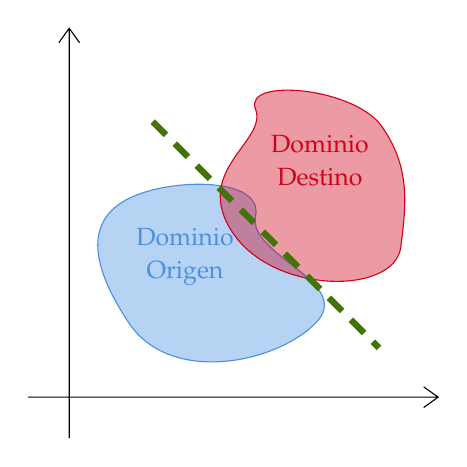
\begin{tikzpicture}[x=0.75pt,y=0.75pt,yscale=-1,xscale=1]
            \draw  (0,177.75) -- (197.5,177.75)(19.75,0) -- (19.75,197.5) (190.5,172.75) -- (197.5,177.75) -- (190.5,182.75) (14.75,7) -- (19.75,0) -- (24.75,7)  ;
            \draw  [color={rgb, 255:red, 74; green, 144; blue, 226 }  ,draw opacity=1 ][fill={rgb, 255:red, 74; green, 144; blue, 226 }  ,fill opacity=0.4 ] (48.5,82) .. controls (68.5,72) and (113.5,71.5) .. (109.5,90.5) .. controls (105.5,109.5) and (157.5,122.5) .. (138.5,142) .. controls (119.5,161.5) and (68.5,172) .. (48.5,142) .. controls (28.5,112) and (28.5,92) .. (48.5,82) -- cycle ;
            \draw  [color={rgb, 255:red, 208; green, 2; blue, 27 }  ,draw opacity=1 ][fill={rgb, 255:red, 208; green, 2; blue, 27 }  ,fill opacity=0.4 ] (109.5,39) .. controls (103.5,23.5) and (157.5,28.5) .. (170.5,47.5) .. controls (183.5,66.5) and (182.5,82.5) .. (179.5,105.5) .. controls (176.5,128.5) and (118.5,128.5) .. (98.5,98.5) .. controls (78.5,68.5) and (115.5,54.5) .. (109.5,39) -- cycle ;
            \draw (115,50) node [anchor=north west][inner sep=0.75pt]  [color={rgb, 255:red, 208; green, 2; blue, 27 }  ,opacity=1 ] [align=left] {\begin{minipage}[lt]{36.4pt}\setlength\topsep{0pt}
                    \begin{center}
                        {\small Dominio}\\{\small Destino}
                    \end{center}

                \end{minipage}};
            \draw (50,95) node [anchor=north west][inner sep=0.75pt]  [color={rgb, 255:red, 74; green, 144; blue, 226 }  ,opacity=1 ] [align=left] {\begin{minipage}[lt]{36.4pt}\setlength\topsep{0pt}
                    \begin{center}
                        {\small Dominio}\\{\small Origen}
                    \end{center}

                \end{minipage}};
            \draw [color={rgb, 255:red, 65; green, 117; blue, 5 }  ,draw opacity=1 ][line width=2.25]  [dash pattern={on 6.75pt off 4.5pt}]  (60,45) -- (169,154) ;
        \end{tikzpicture}
        \caption{Dominios distintos, discriminables.}
        \label{fig:dominios-distintos}
    \end{subfigure}
    \hfill
    \begin{subfigure}[h]{0.46\textwidth}
        \centering
        \tikzset{every picture/.style={line width=0.75pt}}

        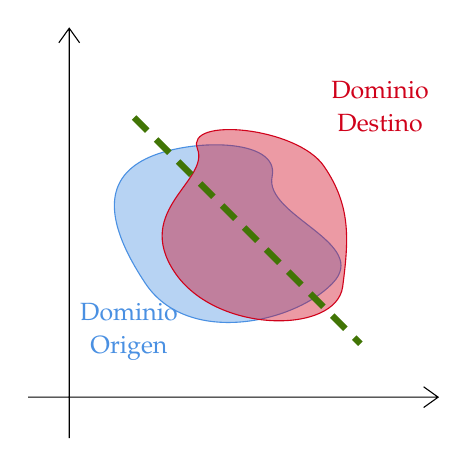
\begin{tikzpicture}[x=0.75pt,y=0.75pt,yscale=-1,xscale=1]
            \draw  (1,179.75) -- (198.5,179.75)(20.75,2) -- (20.75,199.5) (191.5,174.75) -- (198.5,179.75) -- (191.5,184.75) (15.75,9) -- (20.75,2) -- (25.75,9)  ;
            \draw  [color={rgb, 255:red, 74; green, 144; blue, 226 }  ,draw opacity=1 ][fill={rgb, 255:red, 74; green, 144; blue, 226 }  ,fill opacity=0.4 ] (57.5,65) .. controls (77.5,55) and (122.5,54.5) .. (118.5,73.5) .. controls (114.5,92.5) and (166.5,105.5) .. (147.5,125) .. controls (128.5,144.5) and (77.5,155) .. (57.5,125) .. controls (37.5,95) and (37.5,75) .. (57.5,65) -- cycle ;
            \draw  [color={rgb, 255:red, 208; green, 2; blue, 27 }  ,draw opacity=1 ][fill={rgb, 255:red, 208; green, 2; blue, 27 }  ,fill opacity=0.4 ] (82.5,60) .. controls (76.5,44.5) and (130.5,49.5) .. (143.5,68.5) .. controls (156.5,87.5) and (155.5,103.5) .. (152.5,126.5) .. controls (149.5,149.5) and (91.5,149.5) .. (71.5,119.5) .. controls (51.5,89.5) and (88.5,75.5) .. (82.5,60) -- cycle ;
            \draw [color={rgb, 255:red, 65; green, 117; blue, 5 }  ,draw opacity=1 ][line width=2.25]  [dash pattern={on 6.75pt off 4.5pt}]  (52,45) -- (161,154) ;

            \draw (24,133) node [anchor=north west][inner sep=0.75pt]  [color={rgb, 255:red, 74; green, 144; blue, 226 }  ,opacity=1 ] [align=left] {\begin{minipage}[lt]{36.4pt}\setlength\topsep{0pt}
                    \begin{center}
                        {\small Dominio}\\{\small Origen}
                    \end{center}

                \end{minipage}};
            \draw (145,26) node [anchor=north west][inner sep=0.75pt]  [color={rgb, 255:red, 208; green, 2; blue, 27 }  ,opacity=1 ] [align=left] {\begin{minipage}[lt]{36.4pt}\setlength\topsep{0pt}
                    \begin{center}
                        {\small Dominio}\\{\small Destino}
                    \end{center}

                \end{minipage}};
        \end{tikzpicture}

        \caption{Dominios similares, no discriminables.}
        \label{fig:dominios-similares}
    \end{subfigure}

    \caption{Ejemplos de distribuciones de dominios.}
    \label{fig:ejemplos-dist-a}
\end{figure}

Durante el proyecto se utiliza como clasificador una red de una capa densa con una funci\'on de activaci\'on sigmoidea,
es decir, una regresi\'on log\'istica.
\chapter{Análisis de resultados}

\label{Chapter4}

A lo largo del presente capítulo, se analizarán los resultados obtenidos a partir de los experimentos planteados. Se
detallarán las métricas obtenidas, se visualizarán los espacios latentes $\mathbf{z}$ generados por la parte
convolucional de las redes y se analizarán los errores que surgen de aplicar los modelos a los telegramas.

\section{Análisis de métricas}

Los experimentos realizados arrojaron los resultados mostrados en el cuadro \ref{tab:metricas-experimentos}. Las
métricas referidas a la capacidad de clasificación (Accuracy, $F_1$) son evaluadas sobre la partición de test del
dataset de origen donde se conocen las etiquetas a ciencia cierta (MNIST). Por otro lado, las métricas de adaptación
($MMD$, Dist. $\mathcal{A}$) son evaluadas sobre los espacios latentes que los modelos generaron para las particiones
de test de ambos datasets.

Es importante destacar que el mejor modelo es aquel que tiene tanto la mejor capacidad de clasificación como la mejor
adaptación a nuevos conjuntos de datos. Las métricas de clasificación deben ser maximizadas y las de adaptación deben
ser minimizadas.

\begin{table}[H]
    \centering
    \begin{tabular}{cc|rr|rr}
        \toprule
        AD                           & Modelo & Acc.                                & $F_1$                               & $MMD$                               & Dist. $\mathcal{A}$                 \\
        \midrule
        \multirow[c]{2}{*}{-}        & ResNet & {\footnotesize (2)} 0.9885          & {\footnotesize (2)} 0.9883          & 0.0632                              & 1.9306                              \\
                                     & LeNet  & 0.9811                              & 0.9810                              & 0.0469                              & 1.9515                              \\\hline
        \multirow[c]{2}{*}{DANN}     & ResNet & \textbf{{\footnotesize (1)} 0.9890} & \textbf{{\footnotesize (1)} 0.9890} & 0.1379                              & 1.9776                              \\
                                     & LeNet  & 0.9822                              & 0.9821                              & {\footnotesize (3)} 0.0090          & 1.6774                              \\\hline
        \multirow[c]{2}{*}{ADDA}     & ResNet & 0.9476                              & 0.9485                              & 0.0165                              & 1.8495                              \\
                                     & LeNet  & 0.9191                              & 0.9184                              & 0.0399                              & 1.8495                              \\\hline
        \multirow[c]{2}{*}{DANN+BSP} & ResNet & 0.9780                              & 0.9777                              & 0.0409                              & 1.7888                              \\
                                     & LeNet  & 0.9859                              & 0.9857                              & {\footnotesize (2)} 0.0051          & {\footnotesize (3)} 1.6369          \\\hline
        \multirow[c]{2}{*}{MDD}      & ResNet & {\footnotesize (3)} 0.9864          & {\footnotesize (3)} 0.9863          & 0.0615                              & 1.8987                              \\
                                     & LeNet  & 0.9856                              & 0.9854                              & 0.0399                              & 1.7468                              \\\hline
        \multirow[c]{2}{*}{AFN}      & ResNet & 0.9829                              & 0.9827                              & \textbf{{\footnotesize (1)} 0.0040} & \textbf{{\footnotesize (1)} 1.0886} \\
                                     & LeNet  & 0.9862                              & 0.9859                              & 0.0117                              & {\footnotesize (2)} 1.5747          \\

        \bottomrule
    \end{tabular}
    \caption{Métricas de los experimentos realizados. Entre paréntesis se encuentra la posición que ocupa dentro del top 3 de la columna.}
    \label{tab:metricas-experimentos}
\end{table}

Se observa que los modelos entrenados sin adaptación de dominio presentan las mejores métricas de clasificación, como
se esperaba. Sin embargo, estos modelos tienen los peores valores de adaptación, lo que hace que no puedan
generalizarse a nuevos conjuntos de datos, como TDS.

El modelo ResNet, utilizando AFN, demuestra ser el modelo que combina mejor las métricas de clasificación y adaptación.
A pesar de esto, se destaca que los modelos LeNet entrenados con DANN y AFN obtuvieron buenas métricas en general, lo
que sugiere que en ocasiones, un modelo más complejo no necesariamente garantiza un mejor rendimiento.

Los modelos se aplicaron a todos los telegramas, y se calculó el promedio de $IoU$ por telegrama utilizando el método
descrito en el capítulo \ref{Chapter3}. Además, se determinó la cantidad promedio de aciertos por telegrama utilizando
las etiquetas transcritas en el centro de cómputo, asumiendo que hay pocos errores en ellas.

\begin{table}[H]
    \centering
    \begin{tabular}{cc|rrr}
        \toprule
        AD                           & Modelo & $IoU$ prom.     & \# aciertos prom. & \% aciertos prom. \\
        \midrule
        \multirow[c]{2}{*}{-}        & ResNet & 0.4494          & 4                 & 22\%              \\
                                     & LeNet  & 0.4715          & 6                 & 33\%              \\\hline
        \multirow[c]{2}{*}{DANN}     & ResNet & 0.6941          & 12                & 67\%              \\
                                     & LeNet  & 0.7024          & 12                & 67\%              \\\hline
        \multirow[c]{2}{*}{ADDA}     & ResNet & 0.6763          & 11                & 61\%              \\
                                     & LeNet  & 0.6406          & 10                & 56\%              \\\hline
        \multirow[c]{2}{*}{DANN+BSP} & LeNet  & 0.6695          & 11                & 61\%              \\
                                     & ResNet & 0.6515          & 11                & 61\%              \\\hline
        \multirow[c]{2}{*}{MDD}      & ResNet & 0.5451          & 8                 & 44\%              \\
                                     & LeNet  & 0.5801          & 9                 & 50\%              \\\hline
        \multirow[c]{2}{*}{AFN}      & ResNet & \textbf{0.7486} & \textbf{13}       & \textbf{72\%}     \\
                                     & LeNet  & 0.6493          & 11                & 61\%              \\
        \bottomrule
    \end{tabular}
    \caption{IoU promedio y cantidad promedio de aciertos al aplicar los modelos a cada telegrama.}
    \label{tab:iou-cant-aciertos-en-telegramas}
\end{table}

En el cuadro \ref{tab:iou-cant-aciertos-en-telegramas}, se confirma la elección del mejor modelo mencionado
previamente. Es importante destacar que independientemente de la técnica de adaptación utilizada, todos los modelos
presentan mejores porcentajes de aciertos promedio que aquellos modelos entrenados únicamente con MNIST.

Esto sugiere que la adaptación de dominio es fundamental para obtener un mejor rendimiento en la tarea de clasificación
de telegramas. Los modelos entrenados con técnicas de adaptación logran generalizar mejor y son más efectivos en la
tarea de reconocimiento de los patrones presentes en los telegramas, incluso en presencia de ruido y variaciones en los
datos de entrada.

% TODO: aca antes ponia la distribucion de aciertos por modelo y ad. No se que tanto aporta porque tienen la misma
% distribucion que el grafico IoU de analisis de errores.

\section{Análisis de los espacios latentes}

La capacidad de adaptación de dominio es una medida que se utiliza para evaluar el rendimiento de un modelo de
aprendizaje automático en un dominio de prueba diferente al dominio en el que se entrenó. Uno de los factores clave que
influyen en la capacidad de adaptación de dominio es la calidad de los espacios latentes que genera el modelo durante
la etapa de entrenamiento.

El espacio latente en el contexto de las redes convolucionales se refiere a una representación de los datos de entrada
que se ha aprendido durante el entrenamiento del modelo. Durante dicho proceso, la red aprende a extraer
características relevantes de las imágenes de entrada a través de la etapa convolucional.

El espacio latente $\mathbf{z}$ se genera después de la etapa convolucional y antes de la etapa densa de la red. En
este espacio latente, cada dimensión representa una característica específica de la imagen de entrada. Por ejemplo, en
el caso de una red convolucional entrenada para clasificar imágenes de gatos y perros, una dimensión podría representar
la forma de las orejas y otra dimensión podría representar el color de la nariz.

Para evaluar la capacidad de adaptación de dominio de un modelo, se pueden comparar las distribuciones de los espacios
latentes generados para diferentes conjuntos de datos. En general, se espera que los espacios latentes generados para
diferentes conjuntos de datos sean similares, ya que esto indica que el modelo es capaz de generalizar.

Si los espacios latentes son iguales o similares para diferentes conjuntos de datos, la etapa densa de la red que se
encarga de la clasificación puede realizar predicciones precisas para el dominio de destino. Por otro lado, si los
espacios latentes son muy diferentes para diferentes conjuntos de datos, esto puede indicar que el modelo no es capaz
de adaptarse a nuevos conjuntos de datos y, por lo tanto, su capacidad de generalización es limitada.

Una forma común de visualizarlos es mediante una técnica de reducción de dimensionalidad, como Uniform Manifold
Approximation and Projection \parencite{mcinnes2018umap}. UMAP es una técnica no lineal que se utiliza para visualizar estructuras de datos complejas en
un espacio de menor dimensión.

Al visualizar los espacios latentes utilizando UMAP, se pueden observar patrones y relaciones en los datos que de otra
manera serían difíciles de detectar. Al comparar las distribuciones de los espacios latentes generados por un modelo
para diferentes conjuntos de datos, se pueden identificar las similitudes y diferencias entre los dominios, lo que
puede ser útil para evaluar la capacidad de adaptación de dominio del modelo.

En las siguientes subsecciones se analizarán las representaciones UMAP de los espacios latentes obtenidos por cada
modelo entrenado.

\subsection{LeNet}

La figura \ref{fig:umaps-lenet} a continuación contiene las representaciones UMAP obtenidas de los espacios latentes
generados por todos los modelos LeNet.

\begin{figure}[H]
    \centering
    \begin{subfigure}[h]{0.40\textwidth}
        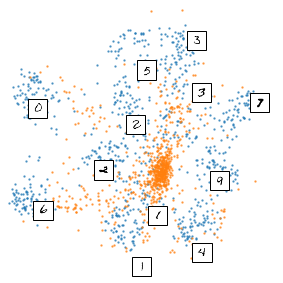
\includegraphics[height=1\textwidth]{chapter4/umap-lenet-so.png}
        \caption{LeNet entrenada con MNIST.}
        \label{fig:umap-lenet-so}
    \end{subfigure}
    \hfill
    \begin{subfigure}[h]{0.40\textwidth}
        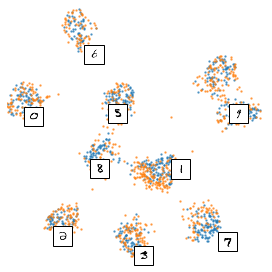
\includegraphics[height=1\textwidth]{chapter4/umap-lenet-dann.png}
        \caption{LeNet entrenada mediante DANN.}
        \label{fig:umap-lenet-dann}
    \end{subfigure}
    \hfill
    \begin{subfigure}[h]{0.40\textwidth}
        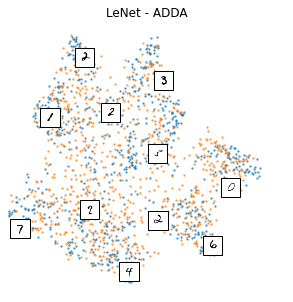
\includegraphics[height=1\textwidth]{chapter4/umap-lenet-adda.png}
        \caption{LeNet entrenada mediante ADDA.}
        \label{fig:umap-lenet-adda}
    \end{subfigure}
    \hfill
    \begin{subfigure}[h]{0.40\textwidth}
        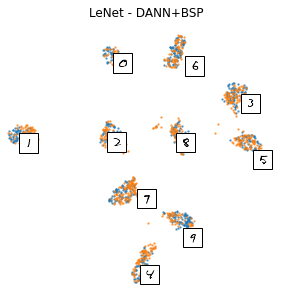
\includegraphics[height=1\textwidth]{chapter4/umap-lenet-bsp.png}
        \caption{LeNet entrenada mediante DANN+BSP.}
        \label{fig:umap-lenet-bsp}
    \end{subfigure}
    \hfill
    \begin{subfigure}[h]{0.40\textwidth}
        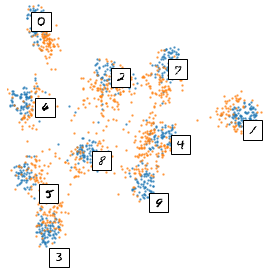
\includegraphics[height=1\textwidth]{chapter4/umap-lenet-mdd.png}
        \caption{LeNet entrenada mediante MDD.}
        \label{fig:umap-lenet-mdd}
    \end{subfigure}
    \hfill
    \begin{subfigure}[h]{0.40\textwidth}
        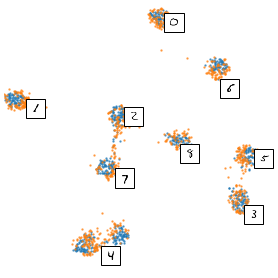
\includegraphics[height=1\textwidth]{chapter4/umap-lenet-afn.png}
        \caption{LeNet entrenada mediante AFN.}
        \label{fig:umap-lenet-afn}
    \end{subfigure}

    \caption{Representaciones UMAP de los espacios latentes de los modelos LeNet. Los puntos azules representan observaciones de MNIST y los naranjas de TDS.}
    \label{fig:umaps-lenet}
\end{figure}

Se pueden observar los siguientes resultados:

\begin{itemize}
    \item Entrenar el modelo solo con MNIST no permite una buena generalización para TDS, como se muestra en la figura
          \ref{fig:umap-lenet-so}.
    \item Con el entrenamiento mediante ADDA o MDD se comienzan a generar agrupaciones en MNIST, pero no logran generarse de la
          misma manera en TDS, como se puede apreciar en las figuras \ref{fig:umap-lenet-adda} y \ref{fig:umap-lenet-mdd}.
    \item Al entrenar el modelo mediante DANN, se generan agrupaciones similares para ambos conjuntos de datos, como se muestra
          en la figura \ref{fig:umap-lenet-dann}.
    \item Finalmente, al utilizar la técnica de entrenamiento DANN con penalización BSP y AFN, se generan agrupaciones similares
          y más densas para ambos conjuntos de datos, tal como se muestra en las figuras \ref{fig:umap-lenet-bsp} y
          \ref{fig:umap-lenet-afn}.
\end{itemize}

En conclusión, se puede afirmar que la técnica de adaptación de dominio utilizada tiene un gran impacto en el
rendimiento de un modelo LeNet debido a su estructura simple. Entre las diferentes técnicas evaluadas, se puede
observar que DANN+BSP y AFN son las que proporcionan una mejor capacidad de adaptación al modelo LeNet. En general,
estos resultados resaltan la importancia de seleccionar cuidadosamente la técnica de adaptación de dominio adecuada
para un modelo dado a fin de lograr un rendimiento óptimo en diferentes escenarios de aplicación.

\subsection{ResNet}

La figura \ref{fig:umaps-resnet} a continuación contiene las representaciones UMAP obtenidas de los espacios latentes
generados por todos los modelos ResNet.

\begin{figure}[H]
    \centering
    \begin{subfigure}[h]{0.40\textwidth}
        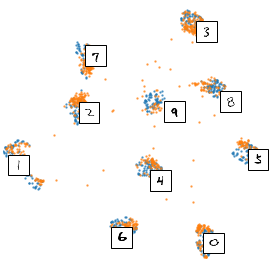
\includegraphics[height=1\textwidth]{chapter4/umap-resnet-so.png}
        \caption{ResNet entrenada con MNIST.}
        \label{fig:umap-resnet-so}
    \end{subfigure}
    \hfill
    \begin{subfigure}[h]{0.40\textwidth}
        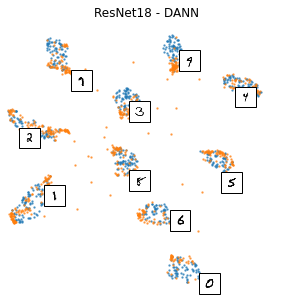
\includegraphics[height=1\textwidth]{chapter4/umap-resnet-dann.png}
        \caption{ResNet entrenada mediante DANN.}
        \label{fig:umap-resnet-dann}
    \end{subfigure}
    \hfill
    \begin{subfigure}[h]{0.40\textwidth}
        \includegraphics[height=1\textwidth]{chapter4/umap-resnet-adda.png}
        \caption{ResNet entrenada mediante ADDA.}
        \label{fig:umap-resnet-adda}
    \end{subfigure}
    \hfill
    \begin{subfigure}[h]{0.40\textwidth}
        \includegraphics[height=1\textwidth]{chapter4/umap-resnet-bsp.png}
        \caption{ResNet entrenada mediante DANN+BSP.}
        \label{fig:umap-resnet-bsp}
    \end{subfigure}
    \hfill
    \begin{subfigure}[h]{0.40\textwidth}
        \includegraphics[height=1\textwidth]{chapter4/umap-resnet-mdd.png}
        \caption{ResNet entrenada mediante MDD.}
        \label{fig:umap-resnet-mdd}
    \end{subfigure}
    \hfill
    \begin{subfigure}[h]{0.40\textwidth}
        \includegraphics[height=1\textwidth]{chapter4/umap-resnet-afn.png}
        \caption{ResNet entrenada mediante AFN.}
        \label{fig:umap-resnet-afn}
    \end{subfigure}

    \caption{Representaciones UMAP de los espacios latentes de los modelos ResNet. Los puntos azules representan observaciones de TDS y los naranjas de MNIST.}
    \label{fig:umaps-resnet}
\end{figure}

Al analizar las representaciones UMAP de los espacios latentes obtenidos por los modelos ResNet, se pueden observar los
siguientes resultados:

\begin{itemize}
    \item En contraste con los modelos LeNet, la ResNet es más eficaz en la extracción de características {\it out of the box},
          lo que le permite generalizar mejor sin necesidad de técnicas de adaptación de dominio (figura
          \ref{fig:umap-resnet-so}).
    \item La aplicación de técnicas de adaptación de dominio como DANN, DANN con penalización BSP y ADDA mejora la capacidad de
          generalización, pero no de forma significativa en comparación con las mejoras obtenidas con LeNet (figuras
          \ref{fig:umap-resnet-dann}, \ref{fig:umap-resnet-bsp} y \ref{fig:umap-resnet-adda}).
    \item El uso de MDD parece disminuir la capacidad de generalización (figura \ref{fig:umap-resnet-mdd}).
    \item La aplicación de AFN potencia la generalización de la ResNet, obteniendo representaciones de los espacios latentes
          prácticamente idénticas para ambos conjuntos de datos (figura \ref{fig:umap-resnet-afn}).
\end{itemize}

En general, estas representaciones permiten visualizar los resultados obtenidos a partir de las métricas de adaptación
descritas en el cuadro \ref{tab:metricas-experimentos} de la sección anterior.

\section{Análisis de errores}

Los errores de predicción de los modelos pueden ser analizados mediante los histogramas de la métrica $IoU$ que se
obtienen de aplicar los modelos a los telegramas.

\begin{figure}[H]
    \centering
    \begin{subfigure}[h]{0.40\textwidth}
        \includegraphics[height=1\textwidth]{chapter4/hist-iou-sin-da.png}
    \end{subfigure}
    \hfill
    \begin{subfigure}[h]{0.40\textwidth}
        \includegraphics[height=1\textwidth]{chapter4/hist-iou-dann.png}
    \end{subfigure}
    \hfill
    \begin{subfigure}[h]{0.40\textwidth}
        \includegraphics[height=1\textwidth]{chapter4/hist-iou-adda.png}
    \end{subfigure}
    \hfill
    \begin{subfigure}[h]{0.40\textwidth}
        \includegraphics[height=1\textwidth]{chapter4/hist-iou-bsp.png}
    \end{subfigure}
    \hfill
    \begin{subfigure}[h]{0.40\textwidth}
        \includegraphics[height=1\textwidth]{chapter4/hist-iou-mdd.png}
    \end{subfigure}
    \hfill
    \begin{subfigure}[h]{0.40\textwidth}
        \includegraphics[height=1\textwidth]{chapter4/hist-iou-afn.png}
    \end{subfigure}

    \caption{Histogramas de la métrica $IoU$ promedio por telegrama por cada técnica AD y modelo.}
    \label{fig:histogramas-ious}
\end{figure}

Resulta interesante mencionar existen telegramas que son más difíciles de analizar que otros. Esto puede evidenciarse
en los histogramas de la figura \ref{fig:histogramas-ious} donde se pueden observar un conjunto de observaciones que
contienen valores entre [0, 0.2] en todos los experimentos realizados. Luego de analizar cada uno de estos casos, se
detectaron las siguientes situaciones:

\begin{itemize}
    \item Telegramas cargados de forma errónea: ver ejemplo en el anexo \ref{anexo:telegrama-erroneo}.
    \item Telegramas correctos pero por alguna cuestión la lógica de extracción de dígitos no funciona correctamente: ver ejemplo
          en el anexo \ref{anexo:telegrama-numeros-juntos}.
    \item Telegramas donde existen otros caracteres distintos a números: al ser un cuadro de texto libre sin formato, los jefes
          de mesa pueden escribir lo que deseen. Ver ejemplo en el anexo \ref{anexo:telegrama-erroneo-caracteres-especiales}
          donde se representa el $0$ a la izquierda con $X$.
    \item Telegramas de mesas donde la mayor cantidad de votos se las lleva un único partido y completan los votos a la izquierda
          con $0$: al agregar los ceros a la izquierda, aumenta la probabilidad de que el modelo se equivoque con esos ceros que
          no aportan al número final. Ver ejemplo en el anexo \ref{anexo:telegrama-erroneo-muchos-ceros}.
\end{itemize}

En los primeros dos puntos se describen problemas problemas que fueron detectados en el proceso de ETL del capítulo
\ref{Chapter3}. Estandarizar los telegramas agregando un casillero por cada dígito junto a mejorar el proceso de
extracción de los mismos, supondrá una mejora considerable en las capacidades predictivas de los modelos.

El tercer punto presenta un problema dentro de la adaptación de dominio. La misma supone que, si bien los datasets de
origen y destino son diferentes pero representan lo mismo, debe existir la misma cantidad de clases entre origen y
destino. Al agregar uno o varios caracteres adicionales en $TDS$ (como es el ejemplo donde representaban el $0$ con una
$X$), se está incumpliendo este supuesto.

El cuarto punto aumenta la probabilidad de error en los modelos debido a que el $0$ a la izquierda no aporta
significado alguno al número de la cantidad de votos que se desea predecir.

Estandarizar la carga de los telegramas por parte de los jefes de mesa mediante alguna capacitación permitiría reducir
los errores de los puntos tres y cuatro en elecciones futuras.


\chapter{Conclusiones}

\label{Chapter5}

La presente tesis se centró en la utilización de técnicas de adaptación de dominio para mejorar la digitalización de de
redes neuronales entrenados con distintos algoritmos de adaptación de dominio. En primera instancia, se desarrolló un
proceso de Extracción, Transformación y Carga (ETL) de los telegramas que permitió segmentar cada uno de los dígitos y
crear un conjunto de datos adecuado para la tarea de digitalización. Este proceso de ETL estandarizó los datos para que
pudieran ser procesados y analizados de manera más efectiva.

En una siguiente etapa, tras realizar múltiples experimentos, se pudo determinar que la red ResNet18 entrenada mediante
AFN es el modelo que tiene el mejor rendimiento en la tarea de digitalización de telegramas. Este resultado indica que
el uso de modelos más complejos y profundos puede ser beneficioso en este tipo de tarea. Sin embargo, también se pudo
comprobar que una red más simple, como la LeNet5 con AFN, tiene un rendimiento satisfactorio, lo que sugiere que no
siempre es necesario utilizar modelos complejos para resolver tareas como ésta.

En cuanto a la precisión obtenida al aplicar el mejor modelo a los telegramas de prueba, se alcanzó una precisión
promedio del 73\%, sin haber estandarizado la casilla donde se escriben los dígitos. No obstante, se podría mejorar aún
más el resultado si se dispusiera de un casillero por número a escribir, lo que permitiría evitar agregar ceros a la
izquierda y, en consecuencia, aumentar la calidad del proceso de ETL de segmentación de dígitos. En este sentido, se
espera que la implementación de esta mejora contribuya a mejorar la precisión de las predicciones.

Es importante destacar que la utilización de técnicas de adaptación de dominio en la tarea de digitalización de
telegramas de elecciones es un campo de investigación en desarrollo, y aún existen diversas limitaciones que deben ser
abordadas. No obstante, los resultados obtenidos en esta tesis son prometedores y sugieren que la adaptación de dominio
puede ser una técnica útil para mejorar la digitalización de telegramas de elecciones en contextos de alta
variabilidad.

Cabe señalar que los resultados obtenidos en esta tesis pueden tener implicaciones importantes en la automatización de
procesos electorales, lo que puede mejorar la eficiencia y la transparencia de las elecciones. Con la digitalización de
telegramas de manera efectiva, es posible mejorar la velocidad y la precisión del conteo de votos, lo que puede reducir
la posibilidad de errores humanos y aumentar la confianza en los procesos electorales.

\section{Trabajos Futuros}

Existen diversas posibilidades de mejora y trabajos futuros que pueden llevarse a cabo para ampliar el alcance y la
calidad de los resultados. A continuación, se detallan algunas posibles líneas de investigación futura:

\begin{itemize}
      \item Mejora del proceso ETL: Una de las limitaciones de la presente investigación es la calidad del conjunto de datos TDS,
            ya que presenta ciertas limitaciones en términos de segmentación de los dígitos en los telegramas. Por lo tanto, una
            posible línea de investigación futura es la mejora del proceso ETL para mejorar la segmentación de los dígitos y
            mejorar la calidad del conjunto de datos.
      \item Mejorar el proceso de post-procesamiento de las predicciones: En la implementación actual, no se realizó ningún tipo de
            post-procesamiento en las predicciones obtenidas por los modelos de aprendizaje automático. Sería útil explorar
            distintas opciones de post-procesamiento, como la validación de que la cantidad total de votos predichos por telegrama
            no supere el total que debe haber por mesa, o la validación de que la cantidad de votos por partido no supere el total
            de la mesa. También se podría considerar la utilización de otras técnicas de post-procesamiento, como la corrección de
            errores en las predicciones mediante la incorporación de información contextual adicional.
      \item Mejora de la estandarización de los telegramas: Como se mencionó en las conclusiones, la estandarización en la sección
            donde se escriben los dígitos podría mejorar aún más la precisión de los modelos de ya que mejoraría la calidad de TDS.
      \item Evaluación de otras técnicas de adaptación de dominio: En esta tesis se evaluaron algunas técnicas de adaptación de
            dominio, pero existen muchas otras técnicas que podrían ser útiles para mejorar la precisión de la digitalización de
            telegramas. Por lo tanto, una posible línea de investigación futura es la evaluación de otras técnicas de adaptación de
            dominio para comparar su efectividad con las técnicas utilizadas en esta investigación.
      \item Evaluación de modelos híbridos: Otra posible línea de investigación futura es la evaluación de modelos híbridos que
            combinen técnicas de adaptación de dominio con otros métodos de mejora de la precisión en la tarea de digitalización de
            telegramas. Por ejemplo, se podría explorar la combinación de redes neuronales con técnicas de procesamiento de
            imágenes para mejorar la calidad de los datos.
\end{itemize}

En conclusión, existen varias líneas de investigación desprendidas de la tesis actual que pueden ser exploradaspara
mejorar la precisión de los modelos que deben aplicarse en un conjunto de datos con características distintas que del
que se entrenó. Estas mejoras pueden ser importantes para aumentar la confianza en los procesos electorales y mejorar
la transparencia y la eficiencia en el conteo de votos.

%----------------------------------------------------------------------------------------
%	THESIS CONTENT - APPENDICES
%----------------------------------------------------------------------------------------

\appendix % Cue to tell LaTeX that the following "chapters" are Appendices

\chapter{Anexo: Telegramas}

\label{anexo:telegramas}

\section{Ejemplo de telegrama}

\includegraphics[width=1\textwidth, height=0.8\textheight, scale=1]{appendices/telegrama.jpg}

%----------------------------------------------------------------------------------------
%	BIBLIOGRAPHY
%----------------------------------------------------------------------------------------

\printbibliography[heading=bibintoc]

%----------------------------------------------------------------------------------------

\end{document}

